\documentclass[a4paper,12pt,french]{report}


% Options possibles : 10pt, 11pt, 12pt (taille de la fonte)
%                     oneside, twoside (recto simple, recto-verso)
%                     draft, final (stade de développement)


%
%%%%%%%%%%%%%%%%%%%%%%%%%%%%%%%%%%%%%%%%%
%%           Liste des packages         %
%%%%%%%%%%%%%%%%%%%%%%%%%%%%%%%%%%%%%%%%%

\usepackage[english, francais]{babel}  
\usepackage[utf8]{inputenc}
\usepackage[T1]{fontenc}
\usepackage{cite}

%\usepackage[babel=true]{csquotes}

\usepackage{color}

\usepackage[normalem]{ulem}
\usepackage{soul}
%\usepackage[pdftex,colorlinks=true,linkcolor=blue,citecolor=green,pagebackref=true]{hyperref}
\usepackage[colorlinks=true,linkcolor=blue,citecolor=lblue,pagebackref]{hyperref}

\usepackage[french]{minitoc}
\usepackage{textcomp}
\usepackage{lmodern}
\usepackage{xspace}
\usepackage[final]{pdfpages}
\usepackage{appendix}
\usepackage{geometry}  
\usepackage[width=0.9\textwidth]{caption}
\usepackage{array}
\usepackage{url}
\usepackage{fancyhdr}
% permet de faire une table des matieres par chapitre
\usepackage{lipsum}
\usepackage[french]{minitoc}


%%%%%%%%%%%%%%%%%%%%%%%%%%%%%%%%%%%%%%%%%
%%           new commands         %
%%%%%%%%%%%%%%%%%%%%%%%%%%%%%%%%%%%%%%%%%

%\newcommand{\com}[1]{{\color{red}\emph{#1}}}
\definecolor{lblue}{rgb}{0,0,0.2}

\newcommand{\alp}{\texorpdfstring{\ensuremath{\upalpha}\xspace}{alpha }}
\newcommand{\bet}{\texorpdfstring{\ensuremath{\upbeta}\xspace}{b\'{e}ta }}
\newcommand{\alpbet}{\texorpdfstring{\ensuremath{\upalpha-\upbeta}\xspace}{alpha-b\'{e}ta}}
\newcommand{\alpt}{\ensuremath{\alpha_2}\xspace}
\newcommand{\strt}{\gls{strt}\xspace}



\newcommand{\g}[1]{\textbf{#1}}  % à mettre en valeur
\newcommand{\T}[1]{\underline{#1}}
\newcommand{\TT}[1]{\underline{\underline{#1}}}
\newcommand{\TTT}[1]{\underline{\underline{\underline{#1}}}}



%%%%%%%%%%%%%%%%%%%%%%%%%%%%%%%%%%%%%%%%%%%%%%%%%%%%%%%%%%%%%%%%%%%%%%

%%\usepackage[square,sort&compress,sectionbib]{natbib}		% Doit être chargé avant babel
%\usepackage[square,sort,comma,numbers]{natbib}
%\usepackage{chapterbib}
%	\renewcommand{\bibsection}{\section{Références}}		% Met les références biblio dans un \section (au lieu de \section*)
%		

%\usepackage{lmodern}
%\usepackage{ae,aecompl}										% Utilisation des fontes vectorielles modernes
%\usepackage[upright]{fourier}
%
%
%
%%%%%%%%%%%%%%%%%%%%%%%%%%%%%%%%%%%%%%%%%%%%%%%%%%%%%%%%%%%%%%%%%%%%%%
%
%%%%%%%%%%%%%%%%%%%%%%%%%%%%%%%%%%%%%%%%%
%%           Apparence         %
%%%%%%%%%%%%%%%%%%%%%%%%%%%%%%%%%%%%%%%%%          
\pagestyle{fancy}
\fancyhf{}
\renewcommand{\chaptermark}[1]{\markboth{\bsc{\chaptername~\thechapter{} :} #1}{}}
\renewcommand{\sectionmark}[1]{\markright{\thesection{} \ #1}}
\renewcommand{\headrulewidth}{0pt}
\lhead[]{\textsl{\rightmark}}
\rhead[\textsl{\leftmark}]{}
\cfoot[\thepage]{\thepage}

\NoAutoSpaceBeforeFDP





%%%%%%%%%%%%%%%%%%%%%%%%%%%%%%%%%%%%%%%%%%%%%%%%%%%%%%%%%%%%%%%%%%%%%%
%
%%% Maths                         
\usepackage{amsmath}			% Permet de taper des formules mathématiques
\usepackage{amssymb}			% Permet d'utiliser des symboles mathématiques
\usepackage{amsfonts}			% Permet d'utiliser des polices mathématiques
\usepackage{nicefrac}
\usepackage{upgreek}			% For roman (i.e. upright) lowercase Greek characters
%
%%%%%%%%%%%%%%%%%%%%%%%%%%%%%%%%%%%%%%%%%%%%%%%%%%%%%%%%%%%%%%%%%%%%%%
%
%
%%% Tableaux
\usepackage{multirow}
\usepackage{booktabs}
\usepackage{colortbl}
\usepackage{tabularx}
\usepackage{multirow}
\usepackage{threeparttable}
\usepackage{etoolbox}
%	\appto\TPTnoteSettings{\footnotesize}
%\addto\captionsfrench{\def\tablename{{\textsc{Tableau}}}}	% Renome 'table' en 'tableau'
%
%            
%            
%
%%%%%%%%%%%%%%%%%%%%%%%%%%%%%%%%%%%%%%%%%%%%%%%%%%%%%%%%%%%%%%%%%%%%%%
%%% Graphiques         
           
\usepackage{subfig}
\usepackage{graphicx}
\usepackage{epstopdf}

%\usepackage{subcaption}
%\usepackage{pdfpages}
%\usepackage{rotating}
%\usepackage{pgfplots}
%	\usepgfplotslibrary{groupplots}
%\usepackage{tikz}
%	\usetikzlibrary{backgrounds,automata}
%	\pgfplotsset{width=7cm,compat=1.3}
%	\tikzset{every picture/.style={execute at begin picture={
%   		\shorthandoff{:;!?};}
%	}}
%	\pgfplotsset{every linear axis/.append style={
%		/pgf/number format/.cd,
%		use comma,
%		1000 sep={\,},
%	}}
%\usepackage{eso-pic}
%\usepackage{import}
%\usepackage{cclicenses}
%
%%%%%%%%%%%%%%%%%%%%%%%%%%%%%%%%%%%%%%%%%%%%%%%%%%%%%%%%%%%%%%%%%%%%%%
%% Biblio                        
%%\makeatletter
%%\patchcmd{\BR@backref}{\newblock}{\newblock(page~}{}{}	% Pour les back-references, affiche 'page' au lieu de 'p.'
%%\patchcmd{\BR@backref}{\par}{)\par}{}{}
%%\makeatother
%	
%	
%%%%%%%%%%%%%%%%%%%%%%%%%%%%%%%%%%%%%%%%%%%%%%%%%%%%%%%%%%%%%%%%%%%%%%
%%% Navigation dans le document   
%\usepackage[pdftex,pdfborder={0 0 0},
%			colorlinks=true,
%			linkcolor=blue,
%			citecolor=red,
%			pagebackref=true,
%			]{hyperref} %Créera automatiquement les liens internes au PDF
%
%
%%%%%%%%%%%%%%%%%%%%%%%%%%%%%%%%%%%%%%%%%%%%%%%%%%%%%%%%%%%%%%%%%%%%%%
%%% Mise en forme du texte        
%\usepackage{xspace}
%\usepackage[load-configurations = abbreviations]{siunitx}
%	\DeclareSIUnit{\MPa}{\mega\pascal}
%	\DeclareSIUnit{\micron}{\micro\meter}
%	\DeclareSIUnit{\tr}{tr}
%	\DeclareSIPostPower\totheM{m}
%	\sisetup{
%	locale = FR,
%	  inter-unit-separator=$\cdot$,
%	  range-phrase=~\`{a}~,     	% Utilise le tiret court pour dire "de... à"
%	  range-units=single,  			% Cache l'unité sur la première borne
%	  }
%\usepackage{chemist}
%\usepackage[version=3]{mhchem}
%\usepackage{textcomp}
%\usepackage{numprint}
%\usepackage{array}
%\usepackage[acronym,xindy,toc,numberedsection]{glossaries}
%	\newglossary[nlg]{notation}{not}{ntn}{Notation} 	% Création d'un type de glossaire 'notation'
%	\makeglossaries
%	\loadglsentries{Glossaire}							% Utilisation d'un fichier externe pour la définition des entrées (Glossaire.tex)
%\usepackage{hyphenat}
%
%
%%% Rajouter en plus du template pour moi :
\usepackage{lipsum}
\usepackage{scrhack}
\usepackage{amssymb}
\usepackage{mathrsfs,amsthm}
\usepackage{calrsfs}
\usepackage{mathtools}
\usepackage[overload]{empheq}
\usepackage{cases} 
\usepackage{multicol}
\usepackage{makeidx}
\usepackage[nottoc]{tocbibind} % ajoute (entre autre) la bibliographie dans la table des matieres 
\usepackage{float}
\usepackage{braket}
%\usepackage[font=small,labelfont=bf,justification=justified]{caption}
%
%%%%%%%%%%%%%%%%%%%%%%%%%%%%%%%%%%%%%%%%%%%%%%%%%%%%%%%%%%%%%%%%%%%%%%
%%% Compilation
%
%\usepackage{silence}
%
%
%%% Virer les erreur dues à minitoc
%\WarningFilter{minitoc(hints)}{W0023}
%\WarningFilter{minitoc(hints)}{W0024}
%\WarningFilter{minitoc(hints)}{W0028}
%\WarningFilter{minitoc(hints)}{W0030}
%
% 
%
%
%%%%%%%%%%%%%%%%%%%%%%%%%%%%%%%%%%%%%%%%%
%%           Page de garde              %
%%%%%%%%%%%%%%%%%%%%%%%%%%%%%%%%%%%%%%%%%
\makeatletter
\def\@ecole{école}
\newcommand{\ecole}[1]{
  \def\@ecole{#1}
}

\def\@specialite{Spécialité}
\newcommand{\specialite}[1]{
  \def\@specialite{#1}
}

\def\@directeur{directeur}
\newcommand{\directeur}[1]{
  \def\@directeur{#1}
}

\def\@encadrant{encadrant}
\newcommand{\encadrant}[1]{
  \def\@encadrant{#1}
}
\def\@jurya{}{}{}
\newcommand{\jurya}[3]{
  \def\@jurya{#1,	& #2	& #3\\}
}
\def\@juryb{}{}{}
\newcommand{\juryb}[3]{
  \def\@juryb{#1,	& #2	& #3\\}
}
\def\@juryc{}{}{}
\newcommand{\juryc}[3]{
  \def\@juryc{#1,	& #2	& #3\\}
}
\def\@juryd{}{}{}
\newcommand{\juryd}[3]{
  \def\@juryd{#1,	& #2	& #3\\}
}
\def\@jurye{}{}{}
\newcommand{\jurye}[3]{
  \def\@jurye{#1,	& #2	& #3\\}
}
\def\@juryf{}{}{}
\newcommand{\juryf}[3]{
  \def\@juryf{#1,	& #2	& #3\\}
}
\def\@juryg{}{}{}
\newcommand{\juryg}[3]{
  \def\@juryg{#1,	& #2	& #3\\}
}
\def\@juryh{}{}{}
\newcommand{\juryh}[3]{
  \def\@juryh{#1,	& #2	& #3\\}
}
\def\@juryi{}{}{}
\newcommand{\juryi}[3]{
  \def\@juryi{#1,	& #2	& #3\\}
}
\makeatother

\newcommand\BackgroundPic{%
	\put(0,0){%
		\parbox[b][\paperheight]{\paperwidth}{%
			\includegraphics[height=0.45\paperheight]{bordure.png}%
			\vfill
		}
	}
}
\newcommand\EtiquetteThese{%
	\put(0,0){%
		\parbox[t][\paperheight]{\paperwidth}{%
			\hfill
			\colorbox{blue}{		
				\begin{minipage}[b]{3em}
					\centering\Huge\textcolor{white}{T\\H\\E\\S\\E\\}
					\vspace{0.2cm}
				\end{minipage}
			}
		}
	}
}

\makeatletter
\newcommand{\pagedegarde}{
\newgeometry{top=2.5cm, bottom=2cm, left=2cm, right=1cm}
\AddToShipoutPicture*{\BackgroundPic}
\AddToShipoutPicture*{\EtiquetteThese}

  \begin{titlepage}
  \centering
      \includegraphics[width=0.4\textwidth]{ParisTech-Institute.pdf}
      \hfill
      \includegraphics[width=0.15\textwidth]{ENSTAlogo}\\
    \vspace{1cm}
      {\Large \'{E}cole doctorale Paris Saclay (EDX)}\\
    \vspace{1cm}
      {\huge 
      	{\bfseries Doctorat ParisTech}\\
    \vspace{0.5cm}
      	TH\`{E}SE}\\
    \vspace{1cm}
   		{\bfseries pour obtenir le grade de docteur délivré par}\\
    \vspace{1cm}
    	{\huge\bfseries \@ecole}\\
    \vspace{0.5cm}
    	{\Large{\bfseries Spécialité: Laser et Matière}}\\
    \vspace{2cm}
    	\textit{présentée et soutenue publiquement par}\\
    \vspace{0.5cm}
    	{\Large {\bfseries \@author}} \\
    \vspace{0.5cm}
    	le \@date \\
    \vfill
       {\LARGE \color[rgb]{0,0,1} \bfseries{\@title}} \\
    \vfill
        Directeur de thèse : {\bfseries \@directeur}\\
        Co-encadrant de thèse : {\bfseries \@encadrant}\\
    \vfill
	\begin{tabular}{>{\bfseries}llr}
		\large Jury\\
		\@jurya
		\@juryb
		\@juryc
		\@juryd
		\@jurye
		\@juryf
		\@juryg
		\@juryh
		\@juryi
	\end{tabular}
	\vfill
	
	\textbf{Thèse préparée au Laboratoire d'Optique Appliquée UMR 7639\\
	ENSTA ParisTech - Ecole Polytechnique - CNRS}

  \end{titlepage}




\restoregeometry  
  
  
}
\makeatother
		% Liste des packages et de leurs options





\let\urlorig\url
\renewcommand{\url}[1]{%
  \begin{otherlanguage}{english}\urlorig{#1}\end{otherlanguage}%
}

% Infos de la page de garde
\usepackage{sectsty}
\allsectionsfont{\centering}



\begin{document}

\selectlanguage{english}
\includepdf{premiereDEcouverture.pdf}
\clearpage
%\dominitoc
%% preparation des minitocs
%
%\dominitoc
%

\clearpage

%\vspace{5cm}
%\pagestyle{empty}
%\begin{center}
%\textit{À mon grand-père}
%\end{center}

%
%\chapter*{Remerciements}
%\begin{center}
%\textit{
%Difficile de savoir dans quel ordre commencer ces remerciements, difficile de n'oublier personne, je tenterai toutefois d'être la plus exhaustive possible et m'excuse d'avance des oublis inévitables et involontaires. Je commence donc par les personnes qui m'ont le plus entourée au laboratoire pendant cette période très enrichissante, à savoir mon groupe PCO et nos amis APPLI: merci donc à Fred, Aurélie, Benoit, Aline et Magalie et Jean-Philippe pour leur soutien sans faille en salle de manip, merci à Maxence pour sa contribution aux simulations et sa disponibilité, merci à Greg et Denis pour leur soutien technique, ainsi que Stephan, Diego, Dominikas et Hermance. Enfin un merci tout particulier Rod et Jérome pour m'avoir permis de travailler dans les meilleurs conditions. Un gros merci au secrétariat pour son dynamisme et sa bonne humeur: Sandrine, Lucie, Octavie, Carole et Patricia. Enfin, un merci bien mérité à la méca, et en particulier à Charlie pour sa bonne humeur et son professionnalisme. Merci également à toutes les autres personnes du Laboratoire, à nos partenaires au CEA, la liste est longue mais merci à tous d'avoir été aussi disponibles, ce sont des années que je n'oublierai pas de si tôt!}\\
%\end{center}
%\begin{center}
%\textit{Je tiens dans un second temps à remercier mes amis, les anciennes ENSTA qui savent ce que c'est de faire une thèse: un gros bisous à Manue, Ananas, Dianou ainsi que Camille et Yves, partis pour le nouveau monde, pour leur soutien! Merci également aux anciennes Saint-Mauriennes qui se seront perdues dans les méandres d'une carrière dans la finance ou le droit des affaires: une grosse pensée pour Camillou, Laura, Ludie et Paula! Finally, a big thank you to my friends from DC and the Thanks-Giving squad: Juanita thank you for being always here ! Ririne, mountains of love all the way to New-Zealand ! Juliette, pleins de bonnes choses pour les années qui arrivent! Merci à toutes et à tous d'être là!}
%\end{center}
%\begin{center}
%\textit{Enfin, un gros merci à ma famille, ma mère qui m'a toujours soutenue et encouragé tout le long de mes études, mon père, pas peu fier, mais à qui je précise tout de même que ma thèse est en physique et non en mathématiques, Laurent qui m'a également toujours soutenu et encouragé. Merci également à mes frères et sœurs pour toujours être restés eux mêmes, ainsi que mon amie d'enfance Valérie qui à toujours été là. J'embrasse toute ma famille au Sénégal et les remercie pour l'accueil chaleureux que j'ai reçu lors de ma dernière visite, merci à toute la famille Bocoum dont je suis fière de faire partie. 
% Enfin, une énorme pensée pour mon grand-père et ma grand-mère qui m'ont également beaucoup soutenu. Je dédie d'ailleurs cette thèse à mon grand-père: ``ça-y-est, je suis r'çue papi''...}
%\end{center}
%
%\begin{center}
%\textit{Merci à tous}
%\end{center}
%
\chapter*{Résumé}

Les rayonnements électromagnétiques ou de particules énergétiques sont d'excellents outils pour sonder la matière qui nous environne. On pense par exemple à l'utilisation des rayons X pour la radiographie ou encore la diffraction pour la compréhension de la structure atomique des cristaux. Toutefois, lorsqu'il s'agit d'étudier la matière à des échelles de temps atomiques (typiquement sub-femtoseconde, $1\,\mathrm{fs}=10^{-15}\mathrm{s}$), les seules sources de rayonnement disponibles restent des installations de grande envergure comme des synchrotrons, avec une résolution temporelle de l'ordre de la picoseconde, ou les lasers à électrons libres, sources parmi les plus intenses, avec des résolutions de l'ordre de la femtoseconde. Depuis une cinquantaines d'années, de nombreux travaux ont été menés pour proposer un jour une alternative reposant sur l'interaction laser-plasma. En effet, lorsqu'un plasma interagit avec une impulsion optique intense ($> 10^{16-17}\mathrm{W/cm^2}$), il en résulte l'accélération de particules (ions,électrons) et l'émission de rayonnement électromagnétique énergétique (X-UV) cohérent. Dans le cadre de cette thèse, ont étudiera la réponse d'un plasma de densité solide lorsqu'il est stimulé par une impulsion d'une dizaine de femtosecondes.\\
 Un plasma est créé sur une cible solide avec un première impulsion de quelques $10^{14}\,\mathrm{W/cm^2}$, dite impulsion pompe. Ce plasma possède une interface avec le vide de qualité optique, si bien qu'il réfléchit en grande partie une seconde impulsion laser, dite impulsion sonde, d'intensité bien plus élevée ($\sim 10^{17-18}\,\mathrm{W/cm^2}$): on parle alors de miroir plasma. C'est la partie non réfléchie de la sonde qui interagira non-linéairement avec ce plasma pour émettre du rayonnement X-UV ou bien libérer les particules accélérées comme des électrons.  Le plasma créé avec la pompe se détend dans le vide à la vitesse du son, si bien qu'il est important de contrôler le délai pompe-sonde de manière précise. En effet, le mécanisme d'interaction avec un plasma peu détendu ($\sim\lambda/100$, donc délai pompe-sonde nul) facilitera l'émission de rayonnement X-UV, alors qu'une fois détendu d'une fraction de la longueur d'onde ($\sim\lambda/10$, donc augmentation du délai pompe-sonde), c'est l'accélération d'électrons qui prédominera. \\

\noindent Dans le premier Chapitre, nous revenons sur le mécanisme de ``Brunel'' décrivant l'interaction d'une impulsion laser avec un miroir plasma. Nous pourrons ainsi expliquer comment le plasma peut émettre une impulsion attoseconde dans la gamme X-UV à chaque cycle optique du laser incident. Ces impulsions optiques interfèrent spectralement pour donner les harmoniques de la fréquence centrale du laser incident: c'est ce qu'on appelle ``génération d'harmoniques''. Les résultats sur la génération contrôlée d'harmoniques seront présentés au chapitre 4. En particulier, on montrera comment l'introduction de couplages spatio-temporels dans le champs laser incident permet de faire ressortir des informations sur le profil temporel du train d'impulsion attosecondes issu de l'interaction. Nous effectuerons un parallèle avec des mesure type FROG (\textit{Frequency-Resolved Optical Gating}), technique de mesure bien connue pour les impulsions laser ultracourtes, fondé sur un algorithme de reconstruction. \\

\noindent Au chapitre 6, nous exposons un des résultats majeur de cette thèse: en changeant la longueur caractéristique du plasma avec lequel notre laser interagit, il est possible de façon sélective ou bien de générer des harmoniques, ou bien d'accélérer des électrons. Nous expliquons, en s'appuyant sur des simulations numériques comment la charge d'espace en surface du plasma permet d'expliquer cette observation. Cela nous conduira à nous focaliser sur le mécanisme d'accélération d'électrons au chapitre 7, notamment à travers l'observation de la distribution angulaire d'emission des électrons, ainsi que leur spectre en énergie. \\

\noindent La longueur caractéristique plasma étant de quelques fractions de longueur d'onde, aussi nous présentons au chapitre 5 une technique de mesure de l'expansion du plasma développé pendant cette thèse, basé sur l'interférométrie spatiale, et qui nous à permis de calibrer la vitesse d'expansion de notre plasma. Le principe est le suivant: un masque troué périodiquement est inséré dans le trajet de l'impulsion principale, si bien que plusieurs tâches de diffraction s'observent dans le plan focale de la parabole. Uniquement l'ordre 0 de diffraction est réfléchit par le miroir plasma, les autres étant réfléchis sur la surface du solide, si bien qu'au cours de la détente, les modulation du profil d'intensité du champs laser réfléchi, directement lié à un déphasage de l'ordre 0, permettent de remonter à l'expansion du plasma.\\

\noindent Nous décrirons au Chapitre 2, le système laser utilisé pour réaliser ces expériences sur cible solide, délivrant des impulsions de quelques millijoules, $<30\,\mathrm{fs}$ au kHz. La compréhension et le développement de cette chaine à représenté un grande partie du travail de thèse, comme par exemple l'identification d'un processus de conversion de post-pulse en pré-pulse par non linéarité. Toutefois, un seul chapitre sera consacré au laser, l'exposé de cette thèse visant à décrire de la manière la plus exhaustive possible la physique de l'interaction laser-miroir plasma. 

\tableofcontents

\chapter{Introduction}
\thispagestyle{empty}

For over a century, the scientific community has invested efforts into developing energetic particle and X-ray sources. This research was driven by the need to study matter on the atomic scale, or even below, with the investigation of elementary particle behavior. The fluence, duration, or spectral emission range of these sources have to be controlled to guarantee the success of an experiment. A particle beam can be composed of simple atoms or molecules (neutrals) or most commonly electrons or ions. On the scale of a nucleus, we can also find products of nuclear reactions (protons, neutrons) and fundamental particles (quarks, leptons..) as studied at CERN. The study of nuclear and fundamental reactions goes beyond the scope of this work because it requires large-scale accelerators ($\sim$TeV energies), unaccessible to an average laser facility. At the Laboratoire d'Optique Appliquée (LOA), our efforts are directed towards the comprehension and development of laser-driven generators of electromagnetic sources (X-UV\footnote{Extreme Ultraviolet: wavelengths between $10$ and $130\,\mathrm{nm}$} in our case) and  particle accelerators (electrons in our case) through laser-plasma interaction schemes. \\


\section{Why do we study plasmas ?}

A plasma is a state of matter where atoms are dissociated into electrons and positively charged ions either completely or partially. Although natural plasmas are rarely encountered on Earth, it is however the most abundant state in the universe and represents 99.9\% of visible state of matter. Therefore, the study of plasmas allows a better comprehension of our universe.  A plasma is characterized by various parameters among which its electron density and its temperature, provided it has reached thermal equilibrium. A common property of plasmas is their ability to emit electromagnetic and/or particle radiations. This is why astrophysical plasmas can be observed from the Earth. The spectral content of this emission is strongly related to their thermodynamical properties and chemical constituents. For instance, interstellar regions are  low-density plasmas  with less than $1\,\mathrm{electron/cm^3}$ and temperatures between $0.1$ and $100\,\mathrm{eV}$. Most of the spectral emission is in the far infrared. Dense plasmas ($\sim 10^{20-25}\,\mathrm{electron/cm^3}$) are encountered in the core of stars like the Sun, where strong thermonuclear reactions prevent the whole structure from collapsing under its own weight. Stars are classified according to their emission spectra going from infrared (cold stars) to gamma rays (hot and turbulent stars). In addition, very intense particle jets (electrons, protons, nuclear reaction products) coming from stars are directly or indirectly observed to describe the core plasma dynamics on various geological time scales. To generate energetic electromagnetic and particle  radiation in a laboratory, we use lasers to create plasmas with micrometer-sized volumes and with densities and temperatures approaching those found in the core of stars. The lifetime of these plasmas is on the order of $10^{-8}$ second.


%(add zeta puppis in following picture)
\begin{figure}[H]
\begin{center}
\noindent\makebox[\textwidth]{
\includegraphics[width =0.9\textwidth]{../introduction/images/plasmaDiagrams.pdf}}\\
\caption{\label{fig:plasmaDiagrams} Examples of plamas sorted by density and temperature}
\end{center}
\end{figure}

\noindent In the attempt to recreate astrophysical plasmas in a laboratory, we have progressively realized that in addition to understanding better the nature of the radiation coming from space, we are also paving the way towards table-top energetic radiation with countless applications (imaging, spectroscopy, medical therapy, nuclear physics...). Over a century, the scientific community has gone from the study of the universe over geological time scale to the study of micrometric systems over proportionally short time scales.

\section{ Laser-plasma physics: historical context}

Before the 50's, the geophysical and astrophysical community essentially studied plasmas doing spectroscopy of partially ionized gas through electric discharges. 
 Langmuir and Tonks were the first to conduct a parametric investigation of partially ionized mercury in the 1920's~\cite{langmuir1923positive,TonksAndLangmuire}, attractive because of its low ionization potential. But in 1960, the first ruby laser would quickly open the door to laser-driven plasma physics. The first efforts were directed towards the creation of high-density plasmas in order to provoke nuclear fusion reactions. However, controlling fusion reactions was not a new idea in the 60's. Between 1936 and 1939, Atkinson, Bethe and Houtermans~\cite{atkinson,bethe1937nuclear,bethe1939energy} had come up with a classification of light elements eligible for fusion to explain the reactions in the core of stars. With no surprise, these scientists were also part of the Manhattan project in the 1940's. In the 1950's, studies on the control of nuclear reactions using magnetically confined plasmas lead to the conception of reactors called Tokamaks~\cite{artsimovich1945radiation,akhiezer1949interaction,rax2011physique}. Finally, Dawson explained in 1964\cite{dawson1964production} how a short ($\sim \,\mathrm{ns}$)\footnote{$1\,\mathrm{ns} = 10^{-9}\mathrm{s}$} intense ($\sim \,\mathrm{TW}$)\footnote{$1\,\mathrm{TW} = 10^{12}\,\mathrm{W}$, power provided by $\sim 500$ nuclear plants} laser pulse \cite{basov1964conditions,daiber1966laser} was an eligible candidate to initiate thermonuclear reactions inside a solid pellet target. These intensities and durations were precisely accessible to state-of-the-art lasers in the 70's\cite{brueckner1974laser}.
In 1974, the Lawrence Livermore National Laboratory (LLNL) conducted the first experiment part of the ``inertial confinement fusion program'' to demonstrate Deuterium/Tritium ignition, using a 20J,$\sim 10\,\mathrm{ns}$ Nd: glass, 1.06 micron laser. After decades of experimental investigation, it appeared that carefully shaping the laser pulse would reduce the energy necessary to trigger nuclear reactions . More insight into the different times scales involved in the plasma dynamics, from nanosecond to femtosecond (and most recently attosecond) has been gained. \\


\subsection{Plasmas: different time scales}

In Physics, the same system can be studied on different time scales. For instance, one uses thermodynamics to predict the final state of a gas. However, on a time scale much shorter than the collision time between two atoms, one should turn to classical kinematics instead. This is of course also true in plasma physics, where the adequate set of equations used to describe the motion of both ion and electron populations inside the plasma will be radically different depending on the time scale of the interaction. Thermonuclear plasmas inside Tokamaks, for instance, are confined during several seconds. Diffusion, convection  and turbulences occur on time scales varying between $\sim~\mathrm{ns}$ to $<1\mathrm{s}$~\cite{rax2011physique}. Rayleigh instabilities~\cite{rayleigh1878instability} grow by $\sim 1\mathrm{\mu m}$ in $\sim 1 \mathrm{ns}$~\cite{emery1982rayleigh} at the surface of laser-compressed pellets and prevent the ignition of fusion reactions~\cite{betti1998growth}. Note that in the latter example, $1\mathrm{\mu m} / 1\mathrm{ns} = 1\,\mathrm{nm/ps}$, which is the sound velocity inside plasmas~\cite{Kruer1988}. Therefore a fluid model is well suited to describe the plasma on a ns time scale over several microns, or on the picosecond time scale over several nanometers. However, using a fluid approach to predict the plasma evolution during one femtosecond over one picometer no longer makes sense. In this case, we reach the dimension of an atom and the time scale of electron collisions in a dense plasma: collisions can be neglected and the physics is now described by the equation of motion of a single electron. The study of plasmas on femtosecond time scales requires the use of femtosecond laser pulses, and a control of the plasma conditions with nanometer resolution. %Therefore, it becomes clear that improving the temporal resolution of a light source isn't enough if no effort is made to simultaneously increase the spatial resolution of the enagaged process observation


\subsection{Lasers: different time scales}

The comprehension of plasma dynamics is strongly related to the rapid evolution of  laser technologies. The temporal duration\footnote{The temporal duration of a laser pulse is defined by the Full Width of Half Maximum (FWHM) of the pulse in power. For a Gaussian pulse, this power is $\propto \exp(\frac{-4 \ln (2)t^2}{\tau_{fwhm}^2})$} of the laser pulse available from continuous (milliseconds) to ultrashort (femtoseconds) depends on the spectral bandwidth and the phase relation between each spectral component. This is  directly influenced by the properties (losses, dimension) of the laser cavity. The temporal duration of a laser, and simultaneously its maximum  peak power\footnote{Peak power for a pulse of energy $E_0$ and temporal duration $P$ $\approx E_0/\tau_{fwhm}$} can be boosted by two techniques, namely Q-switching and mode-locking.\\

\begin{itemize}
\item[$\bullet$]\g{1960: Q-switching:} By a temporal modulation of the losses, the lasing cavity is successively turned on or off. Many round trips occur in the cavity such that the final energy contained in the pulse exceeds by orders of magnitude that of continuous wave operation.\\
\item[$\bullet$]\g{1960-1970: Laser mode-locking:} Used in the generation of ultrashort ($\sim \mathrm{fs}$ to a few ps) pulses. The gain medium inside the cavity has a large bandwith and all the amplified frequencies superimpose coherently inside the cavity. As a result, they interfere constructively, and the cavity generates a continuous train of very short pulses.
\end{itemize}

\vspace{0.3in}

\noindent In Table~\ref{tab:laserPerfs}, we provide an incomplete list of laser systems with different temporal durations. When energetic pulses are required for a given application, the pulse will in general undergo chirped-pulse amplification (CPA)~\cite{maine1988generation}. However, the word record in laser power today which simultaneously combines (i) an ultrashort (6fs) pulse duration and (ii) a very energetic pulse($\sim 100\,\mathrm{mJ}$)~\cite{mikhailova2011ultra} is based on OPCPA~\cite{dubietis1992powerful}.\\

\begin{table}[H]
\begin{center}
\begin{tabular}{ccc}\toprule
Technology & year & temporal duration \\
\hline
Ruby & 1960 & $\sim \mathrm{ms}$ \\
Nd:YAG & 1964 & $\sim200 \mathrm{\mu s}$ \\
Nd:YAG - Q-switched & 1965 & < 1ns\\
Nd:YAG - mode locked& 1968& $\sim30 \mathrm{ps}$ \\
Nd:YLF- Q-switched & 1992& $\sim100\,\mathrm{ns}$ \\
Nd:YLF- mode locked & 1992& $\sim10 \mathrm{ps}$ \\
He-Ne & 1960 & continuous \\
$\mathrm{CO}_2$ & 1964 & $1-100 \mathrm{ns}$ \\
$\mathrm{CO}_2 $- Q-switched & 1964 & <1ns \\
Ti:sapphire & 1982& $\sim 500$ns \\
Ti:sapphire - mode locked& 1989& <10fs \\
\hline
\end{tabular}
\caption{\label{tab:laserPerfs} Example of different laser performances}
\end{center}
\end{table}



\noindent Q-switched lasers are today widely used for industrial applications involving laser processing of metal and medical applications. However, the first experiments on the generation of coherent X-UV light from plasmas were performed using nanosecond $\mathrm{CO}_2$~\cite{burnett1977harmonic,Carman1981} in the 80's. Those results where attributed to the formation of plasma mirrors and reproduced with shorter and more intense  laser pulses in recent years~\cite{Tarasevitch2000,monot2004high,TheseCedric,borot2011high}.


\section{Plasma mirrors}

\subsection{What is a plasma mirror ?}

A plasma mirror (PM) is by definition a plasma, which is highly reflective for electromagnetic radiation, depending of its spectral content. The lower the laser wavelength $\lambda$, the higher the plasma density $n_e$ needs to be. This is illustrated in Fig~\ref{fig:citicaldensitiy}, where we plot the plasma critical density\footnote{Density at which radiation of wavelength $\lambda$ is reflected by the plasma} $n_c [\mathrm{cm^{-3}}] = (1.1\times 10^{21})/(\lambda[\,\mathrm{\mu m}])^2$ as a function of laser wavelength. To be reflective, just like a mirror, the plasma needs an optical surface quality, which means the surface depth fluctuations should remain $<\lambda$. There are however two fundamental differences between a PM and a standard metallic mirror: the first is the "switchability" of the PM. Because most  materials submitted to a very intense electric field ($\gtrsim 10^{13}\,\mathrm{W/cm^2}$) will ionize on a very short time scale ($\sim fs$), most materials can be "switched" into a mirror, during a time corresponding to the PM lifetime. The second fundamental difference concerns the damage threshold: since the plasma is in ionized form, there is no intrinsic limitation in laser intensity that can be reflected on a PM. Because of these properties, non-linear interactions take place, and with them a new field of intense laser-plasma interaction physics. 





\begin{figure}[H]
\begin{center}
\includegraphics[width =0.6\textwidth]{../introduction/images/citicaldensitiy.pdf}\\
\caption{\label{fig:citicaldensitiy}Critical density as a function of wavelength}
\end{center}
\end{figure}

 \noindent In 1990, Manheimer \cite{Manheimer1991} proposed using plasma mirrors for radar systems to replace phase arrays. Two years later, Robson et al. \cite{Robson1992} realized a plasma mirror for microwaves creating a partially ionized plane in a magnetic field and measured a reflectivity comparable to that of a metallic plane. These experimental proofs of principle have quickly been reproduced at lower wavelengths (near infrared, visible)~\cite{bach1983intensity,Kapteyn1991,nantel1998temporal,mathew1996generation,doumy2004complete,dromey2004plasma} as laser technologies evolved and can now be easily created using table-top compact laser systems. 



%
%\begin{figure}[H]
%\begin{center}
%\includegraphics[width =\textwidth]{../introduction/images/timeEvolutionPlasmas.pdf}\\
%\caption{\label{fig:timeEvolutionPlasmas} }
%\end{center}
%\end{figure}
%
%Dense plasma have many physical properties in common with metals because in both medium, electrons are non bounded to atoms and under the stimulation of electromagnetic radiation, currents inside the bulk have the ability to reflect light if the electronic motion can occurs fast enough with respect to the laser wavelength.

\subsection{Lifetime of a plasma mirror}

Laser-plasma interactions are usually performed under vacuum to prevent non-linear degradation of the laser. Therefore, the PM is created under vacuum using an auxiliary pulse we call prepulse, arriving on the solid target prior to the main laser pulse. Its intensity is high enough to ionize the target. For prepulse intensities of the order of $\sim10^{13-14}\,\mathrm{W/cm^2}$, the plasma temperature is $\sim 100\,\mathrm{eV}$~\cite{kruer1988physics}. The plasma inertia is dominated by the ions and its pressure by the free electrons, who transmit their energy to the ions. As a result, the plasma expands towards vacuum, at a velocity of the order of several nm/ps. Unfortunately, the plasma density is not a step-like function, but rather decays exponentially towards vacuum. Two consequences will therefore result from this expansion: (i) The density quickly drops, and the plasma transitions from "overdense" to "underdense". (ii) The expansion induces distortions of the critical surface, and the optical quality of the plasma-vacuum interface degrades in time. For those reasons, the plasma no longer reflects the main incident pulse if it arrives too late (few ps) after the PM has been triggered.\\

\noindent That being said, one would simply need to reduce the delay between the prepulse and main pulse such that the plasma does not have time to expand. However, this is in general not possible.  Indeed, a laser is a complex system made of several sub-units, and many components can introduce unwanted prepulses, with delays and durations spanning from less than a picosecond to several nanoseconds. In this case, we say the laser "temporal contrast" is degraded. For example, spontaneous emission in an amplifier~\cite{nantel1998temporal} and scattering on gratings~\cite{yan2009optimization} generate incoherent light of nanosecond duration copropagating with the main laser pulse. As a consequence, if no precaution is taken, a sufficient amount of energy is temporally spread before the main pulse, and is enough to ionize any surface through tunnel ionization for moderate electric fields, or over-the-barrier ionization for intense electric fields. Electrons are stripped from  all atoms at the surface of the solid, creating a plasma. This plasma expands in time and as a result of this expansion, the PM is destroyed before the main pulse arrives.\\


\subsection{Plasma mirrors for temporal contrast cleaning}

\noindent The well-recognized use of plasma mirrors so far is to improve the temporal contrast of short and intense pulses~\cite{Kapteyn1991}. The working principle is illustrated in Fig~\ref{fig:contrastCleaning}.  The underlying idea of using a plasma mirror to clean the temporal contrast of a short (fs to ps) laser pulses is precisely to take advantage of the poor laser contrast by creating a plasma mirror. 

\begin{figure}[H]
\begin{center}
\includegraphics[width =\textwidth]{../introduction/images/contrastCleaning.pdf}\\
\caption{\label{fig:contrastCleaning} (a) Incident laser pulse with degraded temporal contrast on anti-reflection coated wafer (b) Same laser pulse after reflection on the PM. Energy before the main pulse has been lost in the process of ionization}
\end{center}
\end{figure}

\noindent The energy ``before'' the main pulse is lost in the ionization process. As a result, the reflected pulse contrast is enhanced~\cite{doumy2004complete} from the instant the PM switches on. 
 



\noindent In Chapter~\ref{chapter:Overall presentation of the laser system}, we present the ``'Salle Noire' laser architechture. Here, we will see that another technique, called XPW (fully described in~\ref{subsection:XPW contrast cleaning}) is used for contrast cleaning of our laser. Therefore, in the work presented in this PhD, we study the other properties of plasma mirrors involving non-linear response to an intense ultrashort laser pulse. In particular, we investigate the generation of X-UV radiation and electron ejection.



\subsection{X-UV emission from plasma mirrors}
 
X-rays can be used to probe the nanostructure of many dense materials (radiography, diffraction), or because of they are an efficient type of ionizing radiation (radiation therapy). It has been known for decades that conventional plasma sources can generate X-rays. When a plasma forms, hot electrons can strip core electrons from colder regions, and as they relax, the ionized atoms emit incoherent X-rays, also called K$\alpha$ emission \cite{murnane1991ultrafast}. Thermal electrons in motion also emit incoherent X-Bremsstrahlung which depends on the plasma temperature. Moreover, positively charged ions also emit in the X-ray region, which has been extensively studied by spectroscopists over the last 50 years. Scientific curiosity aside, one could wonder why generating X-UV photons or energetic electrons ($>100\,\mathrm{keV}$) from PM is relevant at all, given it has been done for decades using conventional techniques such as X-ray tubes. The answer is in two words: temporal resolution.\\

\begin{figure}[H]
\begin{center}
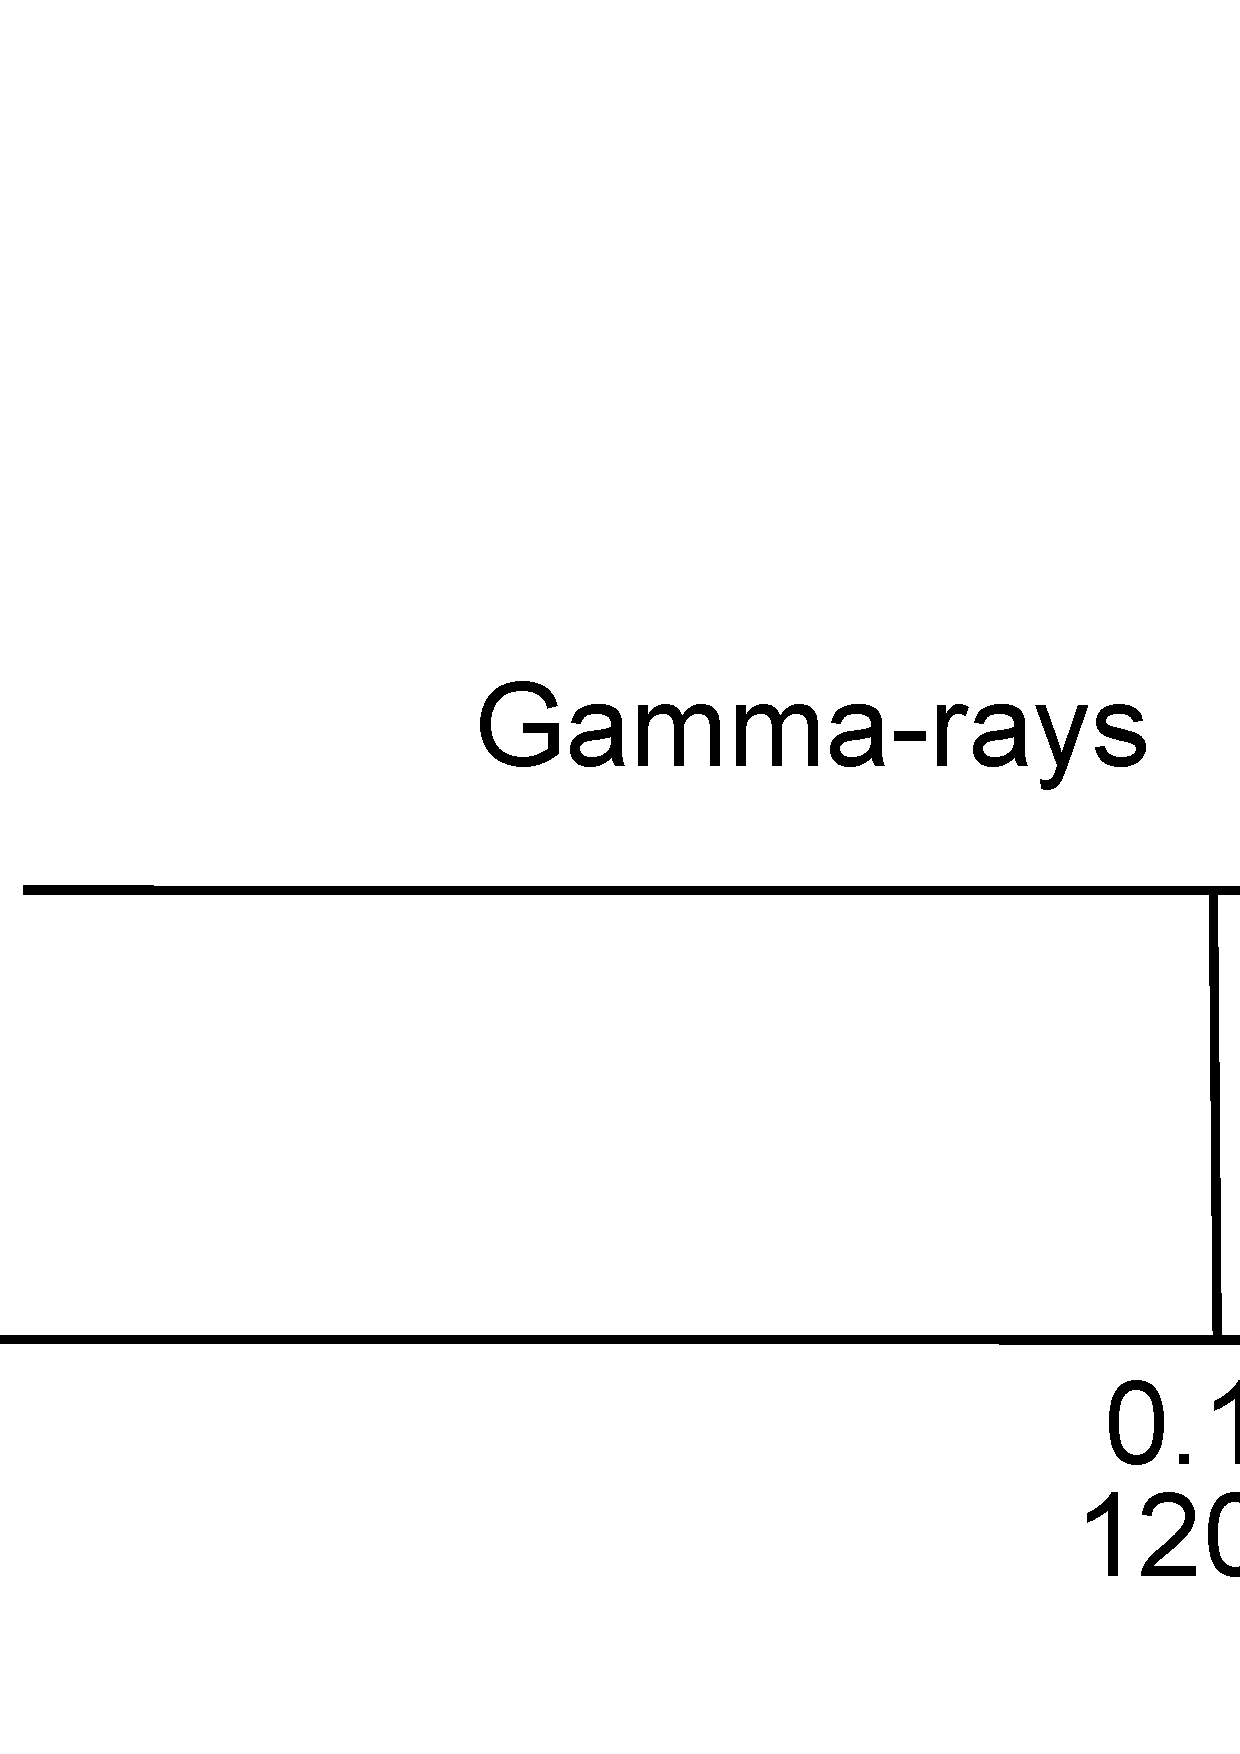
\includegraphics[width =\textwidth]{../introduction/images/spectrum.pdf}
\end{center}
\end{figure}
%
%One property of coherent X-emission is a phase relation between the spectral components of the pulse, which leads to short temporal duration (sub ps to fs) compared to incoherent X emission. Ultimately, fabrication of coherent X-ray sources lead to the study fondamental dynamics of matter such as the vibration of core electron wavefunctions in atoms and molecules or the motion of charged particles in solids or plasmas. 
%
%
%\begin{wrapfigure}
%\begin{center}
%\includegraphics[width =0.5\textwidth]{../introduction/images/Xfel-hamburg}
%\caption{Europeen XFEL facility, Hamburg (http://photon-science.desy.de)}
%\end{center}
%\end{wrapfigure}

\noindent Several conventional facilities can provide intense X-ray radiation. In case of synchrotrons, electrons are accelerated in km-long structures and their trajectories are modified with a combination of magnets (undulators) over a few meters. However, the coherence of such a source is limited and the emission does not go below a few picoseconds, mostly because of the electron bunch duration. Using a femtosecond laser to "slice" the electrons into short pulses, $\sim100\,\mathrm{fs}$ bursts were produced~\cite{schoenlein2000generation} on a synchrotron, but with a limited number of photons.
Free electron lasers (FEL)~\cite{madey1971stimulated,emma2010first,ribic2012status,corde2013femtosecond} are conventional accelerators which can produce intense X-rays~\cite{geloni2010coherence} with peak brightness\footnote{The peak brightness of an X-ray pulse is given in ph/s/0.1\%BW/mm$^2$/mrad$^2$~\cite{corde2013femtosecond}. It is different than the average brightness which accounts for the beam repetition rate} up to one million times greater than on synchrotrons, with pulse durations as short as $\sim 5\,\mathrm{fs}$~\cite{helml2014measuring}.  Although FELs are by far the most reliable installations to generate intense coherent X-rays, their size ($\sim  \,\mathrm{km}$ installations) and effective cost ($\sim G$euros) limit the number of users. In addition, sub-femtosecond X-rays pulses have so far never been achieved.\\

\noindent With the rapid increase of table-top laser peak powers ($> 10^{18}\,\mathrm{W/cm^2}$), it is possible to accelerate electrons in plasmas and generate X-rays. In 1977, Burnett and al. published the first experiment on the generation of X-UV radiation resulting from the interaction of a $\mathrm{CO}_2 $ laser with a plasma mirror~\cite{burnett1977harmonic} called high harmonic generation (HHG). The working principle is as follows: when an intense  laser pulse ($\sim 10^{15}\,\mathrm{W/cm^2}$)  reflects on a PM, electronic motion at the surface leads to the emission of coherent X-UV radiation with attosecond duration, every laser period. This produces a train of attosecond pulses seperated in time by one laser period. Therefore, these pulses interfere constructively in the spectral domain whenever the frequency is a multiple of the driving laser frequency, and for this reason are called high-order harmonics. However, the main limitation of these sources compared to conventional accelerators is the intensity of the source. It is also possible to perform HHG in gas jets with comparable generation efficiencies~\cite{sarukura1991coherent,macklin1993high,l1993high}, and generate X-UV pulses $<100\,\mathrm{as}$~\cite{zhao2012tailoring,goulielmakis2008single}. However, the laser intensity has to remain below the ionization threshold which is an intrinsic limitation of the possible brightness of the sources. On PMs however, the laser intensity can be in principle arbitrarily increased, simultaneously with the  brightness of the generated  X-ray sub-femtosecond bunches.\\

% records:
% FLASH: http://photon-science.desy.de/news__events/news__highlights/archive/archive_of_2006/world_record_at_flash/index_eng.html



%In the ``salle noire'' at LOA is located our sub TW , Ti-Sa laser system delivering a few mJ, $30\,\mathrm{fs}$ to 5$\,\mathrm{fs}$(current upgrade) pulses on target, which allows us to probe plasma dynamics looking at accelerate electrons and the generation X-UV harmonics of the driving laser at a repetition rate of 1kHz. 
% Every $\,\mathrm{ms}$, just before the arrival of the main pulse, the solid target has already turned into a plasma as the transition is fast with respect to the laser pulse ($\sim \,\mathrm{fs}$), but has no time to expand into vacuum (few ps) which makes it optically flat.  This PM is an ideal medium to perform extreme non linear interactions and in particular to generate X-UV coherent light or accelerate electrons and will be extensively disccussed in this manuscript.\\
%

\noindent Classically, a conversion efficiency is an non-dimensional quantity that measures an energy ratio $\eta = E_{out}/E_{in}$ associated with a given physical process. For high harmonic generation on PM, the efficiency is defined for a given frequency range so that $\eta (\omega)$ is an efficiency $/s^{-1}$. We write the energy conservation relation from the temporal to the Fourier domain (Parseval theorem): 

$$
\int_{\mathbb{R}}|E(\omega)|^2\frac{d\omega}{2\pi} = \int_{\mathbb{R}}|E(t)|^2 dt
$$

\noindent where $|E|^2$ is an energy density. Therefore, the energy contained in one attosecond pulse train is given by the harmonic conversion efficiency corresponding to the pulse spectral content. Based on numerical simulations, an integration of the laser energy before and after the interaction on target yields $75$\% reflectivity as presented in Fig~\ref{fig:spectraCamp}. A negligible fraction of the input energy is transfered to the harmonics. 

\begin{figure}[H]
\includegraphics[width =15cm]{../introduction/images/spectraCamp.pdf}\\
\caption{\label{fig:spectraCamp} Illustration of HHG for a 30fs laser pulse with intensity $ I = 10^{18}\,\mathrm{W/cm^2}$ on a PM with a density of 200$n_c$. The percentage of energy of the incident laser contained in the harmonics is given in yellow colors}
\end{figure}
% plasma gradient L/40

\noindent The harmonics shown in Fig~\ref{fig:spectraCamp} are generated with an exponentially decreasing conversion efficiency. This is typical of Coherent Wake Emission mechanism~\cite{Quere2006}, which we will describe in section~\ref{subsection:Plasma perturbative approach}. Here, the energy contained in the harmonics is expected to be linearly increasing with the laser intensity~\cite{plaja1998generation,thaury2010high}. At much higher intensity however, a new mechanism called Relativistic Oscillating Mirror~\cite{Thaury2007} is now responsible for the emission. For this mechanism, it has been predicted that an increase of the laser intensity would simultaneously enhance the generation efficiency~\cite{thaury2010high}. Numerical simulations performed with a laser intensity of $\sim 10^{19}\,\mathrm{W/cm^2}$ indicate that sub-fs X-UV emission can reach several percent~\cite{Naumova2004} (mostly contained in low HHG orders) and therefore compete with peak-brightnesses obtained using X-FEL lasers.


 \subsection{Electron acceleration from plasma mirrors}

 High energy particle radiation started to become an attractive source for various application after the discovery of artificial nuclear reactions between 1910 and 1930. Physicists had access to alpha and beta particles resulting from nuclear reaction products~\cite{rutherford1916xliii}, but were limited in energy and flux. 
 In 1927, Rutherford, publicly announced at the Royal Society of London his ``\textit{ambition to have available for study a copious supply of atoms and electrons which have an individual energy far transcending that of the alpha and beta particles}”. 
 In 1929, Walton and Cockcroft built the first proton accelerator to perform fundamental nuclear experiments by means of a high-voltage static electric field $\sim 10^6\,\mathrm{V}$, accelerating protons up to $300\,\mathrm{keV}$~\cite{cockcroft1930experiments,cockcroft1932experiments}. This was sufficient to manage the transmutation of lithium nuclei, for which they received a Nobel Prize in 1951. Another type of electrostatic accelerator, developed in parallel by Van de Graff consisted in transporting charges in a moving belt, lead to particles accelerated up to $\sim 15\,\mathrm{MeV}$. During the same period, a new type of accelerator invented by Lawrence in 1932, called cyclotron, was born. The principle is to use a magnetic field to confine electrons into a spiral while a radio-frequency electric field $\sim 10^3\,\mathrm{V}$ accelerates them (or other charged particles). 
  After World War II, a variant of cyclotrons called ``synchrotrons'', still widely used today in medical applications, was born. Because the research had been so far mostly driven by nuclear research, most experiments consisted in the acceleration of charged ions. However, electrons which are also charged and almost two thousand times lighter that protons can also be accelerated, and their trajectories are easy to modulate in time. The first electron accelerator principle was proposed by D. W. Kerst in 1940 and was based on betatron acceleration (synchrotron for ``beta'' particles)~\cite{kerst1940acceleration} followed by successful table-top proof-of-principle at the University of Illinois. In 1945, $100\,\mathrm{MeV}$ electrons were accelerated at General Electric based on this principle. Betatron accelerators were for instance used in the Manhattan project to investigate some basic radioactive components properties. Electrons are accelerated in a circular vacuum chamber through an inductive effect: an alternative magnetic field generates an accelerating radial electric field. Note that a betatron and a linear induction accelerator are quite similar with the difference that the trajectories are circular in case of betatrons. In fact, for acceleration to be significant, electrons need to be circulated millions of times in the toroidal chamber, which explains why an additional magnetic field is added to prevent them from escaping their circular orbits of radius $R$.


\begin{equation}
E(\mathrm{MeV}) \le 300 B_s(\mathrm{T}) R(\mathrm{m})
\end{equation}

\noindent For example, an energy of $450\,\mathrm{MeV}$ could be reached theoretically taking $R = 1\,\mathrm{m}$ and $B_{s} = 1.5\,\mathrm{T}$. Betatrons are limited in terms of acceleration because of the finite magnet size and radiation losses of the charged particles, but they have the great advantage of being compact devices, which makes them very appealing for industrial and medical applications.\\

\noindent But since the 80's, laser-driven plasma acceleration techniques have emerged: intense laser pulses focused into a gas jet generates compact accelerating structures where the electric field reaches $\sim $TV/m. The concept of plasma acceleration was introduced by Dawson and Tajima in 1979~\cite{tajima1979laser}. The idea is to focus a beam into a gas jet to generate a micrometer accelerating cavity called wakefield. A wakefield cavity resembles that of a RF linear accelerator, but electric fields are orders of magnitude higher. The use of an energetic electron or ion beam was suggested in 1994 to trigger the fusion reaction of laser compressed deuterium pellets~\cite{tabak1994ignition}. In this so called "fast ignition" scheme, $\sim 1\,\mathrm{MeV}$ suprathermal electrons are produced in the interaction of an intense laser at the surface of the compressed pellets, which propagate towards the core where they deposit their energy. This mechanim, fully supported by simulations~\cite{tabak1994ignition} has not yet been demonstrated experimentally. This initially explained the growing interest of the community in laser-driven solid-density experiments~\cite{honrubia2006three,Brunel1987,Gibbon1992,askar1994magnetic,pukhov1996relativistic,sheng2002stochastic}. In Chapter~\ref{Anticorrelated harmonic and electron emission from plasma mirrors}, we will give a more detailed description of the different mechanisms involved in the interaction of an intense laser beam with a solid density plasma, leading to electron acceleration. \\

\noindent However, as we already mentioned, a solid density plasma is not necessarily a plasma mirror. When the plasma expands into vacuum, its surface quality degrades and the laser interacts with the underdense region of the plasma before it is reflected as described in chapter~\ref{chapter:Laser-solid-plasma interaction: overview}. Few experiments have so far been conducted on the acceleration of electrons from plasma mirrors~\cite{mordovanakis2009quasimonoenergetic,thevenet2015}. The work presented in this PhD focuses on the exploration of this interaction in the sub-relativistic regime. In particular, we will describe the prerequisites for efficiently accelerating electrons from plasma mirrors.



%
%When a laser pulse propagating in vacuum interacts with matter, the electromagnetic energy it carries can either be reflected, transmitted or absorbed. 
%Those three responses usually occur simultaneously and previledge absorption, reflection or transmission will depend on the laser caracteristics (frequency, pulse duration, intensity ..) and on the medium chosen for the interaction (gas,dielectric, metal, plasmas..) as well as the nature of the vacuum/matter interface (polished, plane, periodically structured..). If we consider a solid for the interaction (typical density of $\sim 10^{23}\,\mathrm{atoms/cm^3}$), it is well known that if the laser frequency matches the electron bounding energies of the atoms, the solid is ionized. 
%The study of laser/plasma interactions is more the 50 years old, and laser absorption have often been attributted to collisions between charged particles, which means transforming coherent electromagnetic radiation into thermal energy (joule effect). But up untill the emmergence of mode-locked femtosecond lasers, the typical time scale on which plasmas were investigated was limited to the nansecond (CO2 lasers for instance) and later to the picosecond (Q-switch) timescale which is much greater than the caracterisic time known for collisions ($\sim $ fs). 






\newpage




\section{Brief description of the different chapters}

\begin{itemize}
\item[$\bullet$]  \g{Chapter~\ref{chapter:Laser-solid-plasma interaction: overview} :} In this chapter, we describe the basic mechanism behind laser absorption on thin plasma mirrors. We present in detail the so-called "resonant absorption" mechanism, as well as "Brunel Absorption" mechanism, better suited for plasmas with very short scale lengths. In a second time, we will see how a dense plasma responds to an electronic perturbation by generating X-UV light, and discuss the asymptotic case of very long and very short plasma scale length, where this emission can no longer take place. 

\item[$\bullet$]  \g{Chapter~\ref{chapter:Overall presentation of the laser system}}: In this chapter, we describe the global architecture of our laser. After a brief presentation of the main components, we focus on XPW contrast cleaning and present a source of temporal contrast degradation in our CPA. After discussion on the laser contrast and the possible way of improving it, we describe the solid-target interaction chamber. In particular, we will present the $1 \mathrm{kHz}$ rotating target and the main beam characteristics (spatial, temporal) on target.


\item[$\bullet$]  \g{Chapter~\ref{chapter:Properties of attosecond pulses emitted using plasma mirrors}}: In this chapter, we will recall some of the basic properties of Coherent Wake Emission (CWE). The reader is invited to check the provided references for a more detailed description. In a second part, we will see how the divergence and spectral properties of the emitted harmonics are sensitive to spatio-temporal couplings (STC) of the driving laser. In particular, we will show how it is possible to experimentally control an STC of first order called Wave Front Rotation (WFR) and how it can affect harmonic generation. This technique has been already tested successfully to seperate attosecond pulses from plasma mirror by changing over time their direction of emission~\cite{Wheeler2012}. Here we discuss the possibility of retrieving temporal information on the attosecond train when the pulses are not separated.  


\item[$\bullet$] \g{Chapter~\ref{ch:Measuring the gradient expansion}}: In this chapter we present a technique developed during this PhD called spatial domain interferometry (SDI), which allows us  to measure the expansion velocity of the plasma generated on the solid target by a controlled prepulse. We will then discuss the current limitations of this technique such as the pointing stability of the pulses on target, and how it can be easily identified using the intensity profile of the reflected probe. Finally, we will suggest to go one step further with the implementation of a phase-retrieval algorithm allowing the two-dimensional reconstruction of the plasma during its expansion.


\item[$\bullet$]  \g{Chapter~\ref{Anticorrelated harmonic and electron emission from plasma mirrors}}: In this chapter, we present experimental results of the simultaneous observation of harmonics and electrons from plasma mirrors. In particular, we show how the emission is anticorrelated with the gradient scale length. We then present the measured electron angular emission profile and energy spectra depending on the plasma scale length.




\item[$\bullet$]  \g{Chapter~\ref{Laser-electron interaction in vacumm}}: This chapter focuses on electron interaction with the laser when it reflects on the plasma surface. We discuss two different regimes namely ``ponderomotive'' and ``non ponderomotive'' laser acceleration in vacuum, and in particular how they depend upon the laser intensity. We also discuss the effect of our strong focusing geometry  on the angular emission profile of electrons.

\end{itemize}



































 
%%%%%%%%%%%%%%%%%%%%%%%%%%%%%%%%%%%%%% Accélération d'électrons sur miroir plasma
\chapter{Laser-solid-plasma interaction: overview}\label{chapter:Laser-solid-plasma interaction: overview}
\minitoc

\thispagestyle{empty}

\section{Laser absorption in plasmas}
\label{sec:LaserAbsorptions}

In the early 70's efforts to control thermodynamical reactions using pellet targets\cite{nuckolls1972laser}, unusual surface absorption of the intense pulse light was observed experimentally \cite{self1976lawrence,brueckner1974laser,priedhorsky1981hard}, which was a hint that new nonlinear phenomena where taking place. The invoked mechanism to describe these observations was historically called ``resonant absorption'': the laser propagates in the underdense region of the solid density plasma  surface and reaches a regime called ``wavebreaking''. Here, strong coupling between the laser field and the plasma waves becomes possible. The authors who described this mechanism did not mention the possibility of high-order harmonic generation in the process, but did state that this could explain hot-electron acceleration from solid plasma targets \cite{freidberg1972resonant,albritton1975cold}. This was critical because this hot electron population would preheat the core of the pellet. In the 1993, Tabak~\cite{tabak1994ignition} proposed a fast ignition scheme where those same hot electrons were chosen to trigger nuclear reactions after an adiabatic compression, which is why their emission properties have to be controlled (low divergence, monoenergetic).\\
 In this chapter, we go over the physical concepts of the ``resonant absorption'' model, and highlight the different hypotheses made in order for it to be valid, among which that the plasma scale length should be ``long''. In his famous article called ``not-so-resonant, resonant absorption'' \cite{Brunel1987}, Brunel proposed a model, which we trivially call ``Brunel model'', more applicable in the case of short plasma scale lengths, as described in~\ref{section:Brunel absorption mechanism}.
%: the laser periodically excites electron at the plasma surface. When the laser force is oriented towards the plasma bulk, electrons can propagate deep enough to escape the screened laser field leading to a loss in laser energy (conversion to kinetic energy) . In addition to explain unsually laser absorption, this mechanism will prove to be essential in the modelisation of Coherent Wake Emission harmonics inside the plasma as described further in Chap? . 





\subsection{Resonant absorption}

To go over the basic principles of what is generaly called "resonant absorption", we will start by writing Maxwell's equations for both the magnetic and electric field in a plasma we assume to be non-magnetic ($\g{M}=\g{0}$) and non polar ($\g{P}=\g{0}$). These equations can be found in Appendix~\ref{ch:Normalisation conventions}.

\begin{subequations}
\label{eq:EandBequations}
\begin{align}[left = \empheqlbrace\,]
&\nabla^2 \g{E}(\g{r},t)  - \nabla ( \nabla. \g{E})  - \frac{1}{c^2} \partial_{t}^2 \g{E}(\g{r},t)  -\mu_0\partial_t \g{j}(\g{r},t) = \g{0}  \label{eq:Eequations}\\
&\nabla^2 \g{B}(\g{r},t) - \frac{1}{c^2}\partial_{t}^2 \g{B}(\g{r},t)  + \mu_0\nabla \times \g{j}(\g{r},t) =\g{0} \label{eq:Bequations} 
\end{align}
\end{subequations}

\noindent To close this system of equations, one needs to make a hypothesis about the response of the current $\g{j}$ to an electromagnetic field. We therefore suppose that the plasma of initial electronic density $n_{e0}$ is neutral, and that only the electrons (as opposed to the much heavier ions) are in motion. Moreover, we consider a ``cold'' plasma, which means we study its dynamics on a time scale where collisions can be neglected in the equation of motion. With those conditions met, we can use the non-relativistic equation of motion known for one electron and retrieve the expression of the current using the relation:
$$
\g{j}(r,t) = -en_e(\g{r},t) v_e(\g{r},t)
$$

\subsection{Neutral plasma response equations}

We suppose that the plasma density is independent of time $n_e(\g{r},t) = n_{e0}(\g{r})$. The function $n_{e0}(.)$ is often chosen to be exponentially decreasing towards vacuum as explained further in Chap~\ref{ch:Measuring the gradient expansion}. However, we do not need to make such a hypotheses within the scope of the present derivation.\\
The neutrality of the plasma is imposed at all time, which yields $\nabla \g{j}(\g{r},t) = 0$ because of the charge conservation. The dynamics of the system are described by the non-relativistic equation of motion ($\gamma =1$ and $\g{B}=\g{0}$, as described in Appendix~\ref{ch:Normalisation conventions})

\begin{equation}
\frac{d\g{v}_e}{dt}=\partial_t\g{v}_e + (\g{v}_e\nabla )\g{v}_e = -\frac{e}{m_e}\g{E}(r,t) 
\label{eq:EquationOfMotionNR}
\end{equation}

\noindent To linearize Eq.~\ref{eq:EquationOfMotionNR}, we make the assumption that $v_e<<L \omega_0$ where $L$ is the characteristic scale length of the problem and $\omega_0$ the driving laser frequency. Note that in a homogeneous plasma, $L$ is equal to the driving laser wavelength and that condition is automatically verified, but for strongly inhomogeneous plasmas however, $L$ can be significantly smaller. Assuming the inequality holds true, we have for a monochromatic field:

\begin{subequations}
\label{eq:Jderivation}
\begin{align}[left = \empheqlbrace\,]
&\g{j}(\g{r},\omega) = - n_{e0}(\g{r})\frac{e^2}{i\omega m_e}\g{E}(\g{r},\omega)  \label{eq:PartialJ} \\
&\nabla \times \g{j}(\g{r},\omega) = \frac{-e^2}{i\omega m_e}[\nabla n_{e0} \times \g{E}(\g{r},\omega)+n_{e0} i\omega\g{ B}(\g{r},\omega) ]\label{eq:NablaJ} 
\end{align}
\end{subequations}

\noindent We define:
$$
\omega_p(\g{r})^2 = \frac{n_{e0}(\g{r})e^2}{m_e\epsilon_0}
$$


\noindent By applying the $\nabla.$ operator to the \textit{Maxwell-Ampere} Equation given in ~\ref{eq:Maxwell-Equations}, it is easy to show that $\nabla j =0$ implies $\partial_t (\nabla E) = 0$.
Therefore, supposing the plasma was neutral at time $t=0$, this leads to $\nabla E = 0$ at all times in Eq.~\ref{eq:Eequations}. The
\textit{Maxwell-Ampere} equation in the Fourier domain also gives the relation:

\begin{equation}
\label{eq:Bfield}
\nabla \times \g{B} = \frac{ic^2\omega}{\omega^2-\omega_p(\g{r})^2}\g{E}(\g{r},\omega)
\end{equation}

\noindent  By injecting Eq.~\ref{eq:Bfield}  in Eq.~\ref{eq:EandBequations} and using the relations in~\ref{eq:Jderivation}, we obtain separate equations for $\g{E}$ and $\g{B}$, which are the equations commonly used to propagate the field undergoing ``resonant'' absorption in a plasma:



\begin{subequations}
\label{eq:RAequations}
\begin{align}[left = \empheqlbrace\,]
     &\nabla^2 \g{E}(\g{r},\omega) +  \frac{\omega^2-\omega_p(\g{r})^2}{c^2}\g{E}(\g{r},\omega)=0 \label{eq:RAequations1}\\
     &\nabla^2 \g{B}(\g{r},\omega) - \frac{1}{\omega^2-\omega_p(\g{r})^2}\nabla \omega_p^2 \times \nabla\times \g{B}+ \frac{\omega^2-\omega_p(\g{r})^2}{c^2} \g{B}(\g{r},\omega) =0 \label{eq:RAequations2}
\end{align}
\end{subequations}

\noindent Equation ~\ref{eq:RAequations1} shows the impossibility for the electric field to propagate for $\omega < \omega_p(\g{r})$ (this index is negative, as for a metallic mirror) which defines the \underline{critical surface equation}:
$$
n_e(\g{r})=n_c
$$ 

\noindent Above the critical surface, the electric field gets reflected and below, it becomes evanescent.

\subsection{Geometrical representation of resonant absorption}

Since resonant absorption applies to long gradient scale lengths, it is quite easy to confuse with the geometrical optics picture of a wave curving its $k$ vector along propagation as shown in Fig~\ref{fig:gradient}.

\begin{figure}[H]
\begin{center}
\includegraphics[width =10cm]{../chapitre1/images/gradient.pdf}\\
\caption{\label{fig:gradient} Artistic representation of resonant absorption for a 1-dimensional electron density distribution $n_e(x)$. $\g{k}$ is the incident wave vector and $\theta$ is the incident angle. The field is reflected at the critical surface $n_c$, which coincides with purely normal $\g{E}$ component. This illustration is largely inspired by Figure 2.5 found in~\cite{theseAnto}.}
\end{center}
\end{figure}

\noindent The geometrical representation of a wave propagating in a density plasma, illustrated by Fig~\ref{fig:gradient}, becomes wrong for a short scale length $L$ because the underlying hypotheses behind this representation is that $L >> \lambda$ where $\lambda$ is the driving laser wavelength. Indeed, a representation of an optical wave with $\vec{k}$ changing direction while propagating along $x$ is a geometrical optics representation driven by the eikonal equation \cite{LandauLip}, or in other words the Fermat Principle, and we can write:

\begin{equation}
n(x) \sin\theta(x) = constant
\end{equation}

\noindent That is to say in our case for a propagating wave of frequency $\omega$:

\begin{equation}
(1 - \frac{\omega_p(x)^2}{\omega^2})^{1/2}\sin\theta(x) = \sin(\theta_0)
\end{equation}

\noindent where $\theta$ is expected to increase with x, since $\g{k}$ is directed towards a zone of lower index. In this case, the wave would be refracted by the underdense plasma before it could reach the critical density $n_c$. \\

\noindent This shows that the geometrical approach is incorrect and that propagation in the underdense part  of the plasma, when $L$ is comparable to $\lambda$, needs to be treated using wave equations ~\ref{eq:RAequations}. However, the mental representation given in Fig~\ref{fig:gradient} is still relevant as shown by Freidberg et al. \cite{freidberg1972resonant} who integrated the system of equations ~\ref{eq:RAequations2} for a magnetic field having the form:
$$
B = B_z(x)e^{-i(\omega t - k_y y)}
$$

\noindent where $k_y = \frac{\omega}{c}\sin\theta$ is independent of $x$. The solution in the case of a linear density gradient increasing from $0$ to the critical density is evanescent for $E_y$. This absorption behavior is optimal for a given angle and gradient length ($\theta = 23^{\circ}$ for $L = 1.6 \lambda$). The $E_y$ component of the electric field is rigorously equal to zero at the critical surface while the $E_x$ component of the electric field significantly increases. Therefore: the geometrical representation given in Fig~\ref{fig:gradient} appears correct if instead of picturing the $\g{k}$ vector turning during the propagation, we impose $\theta$ to be constant at all time and instead picture the evanescent $E_y$ component of the electric field.
This singular behavior is associated with a strong coupling of $E_x$ with plasma waves at the critical surface and is responsible for collisionless conversion of the laser energy into electronic kinetic motion~\cite{freidberg1972resonant}.

\noindent The important remark to make about resonant absorption is that the description of a neutral plasma remains valid as long as the scaling law given in Eq.~\ref{eq:Poisson} holds true. In particular, for a plasma at critical density, this implies:
$$
L_0 >> \frac{V_{osc}}{\omega_0}\approx \lambda_0/6
$$

\noindent The numerical estimate is done for a typical electric field of $a_0 = 1$ at $\lambda_0 = 800\,\mathrm{nm}$. In the physical mechanism we consider, the plasma length typically scales as a fraction of the laser wavelength, which is why  a ``Brunel'' absorption model, as presented hereafter, is applicable.






\section{Brunel absorption mechanism}
\label{section:Brunel absorption mechanism}

Brunel's absorption mechanism is crucial in order to understand how the laser beam reflecting off the critical surface can transfer its energy to the plasma without penetrating it. Indeed, up until Brunel's milestone article in 1987 \cite{Brunel1987}, absorption of a short laser pulse ($\mathrm{CO}_2$ lasers with picosecond durations  at the time) by overdense plasmas was mainly attributed to resonant absorption \cite{freidberg1972resonant}. \\

\noindent In Brunel's model, the electrons at the plasma mirror surface respond to the incident laser electric field in such a way that the plasma is no longer considered neutral. At different phase of the driving laser, surface electrons are accelerated towards vacuum following different trajectories, while the much heavier ions remain static. This creates a charge separation field which tends to pull electrons back towards the plasma. As the laser field changes sign, it adds to the ion static field and electrons accelerated in the direction of plasma bulk gain sufficient energy to cross the critical surface and therefore escape the laser influence. As they cross the critical surface with accumulated kinetic energy and "\textit{(...) since the field is null inside, one can see that the kinetic energy given to the particles that reenter the plasma is lost}(Brunel,1987\cite{Brunel1987})", or in other words the laser transfers its energy to the plasma, justifying the term "absorption".

\subsection{Modeling}

A 1-dimensional approach allows one to get an analytical expression of the electron trajectories for a given incident laser field $E_L(t)$ only dependent on time $t$ and defined at the surface of the plasma. We therefore project the electron equation of motion onto the $x$ direction of space and impose $v_y=v_z = 0$ such that:
\begin{equation}
\frac{d(\gamma v_x)}{dt} = -e\underbrace{(\g{E}_I+\g{E}_R).\g{u}_x}_{\mbox{reflection}} - e\underbrace{(v_y B_z - v_z B_y)}_{=0}
\end{equation}

\noindent where $E_I$ and $E_R$ are the incident and reflected fields at the plasma surface. The laser field strength results from their constructive interference such that $E_L(t) = 2E_I(t)\sin\theta$ with the trivial assumption that $|E_I| = |E_R|$.


\noindent Electrons are accelerated away from the critical surface into vacuum creating a space charge field due to the static ions. In result, this space charge field will screen the driving laser field. To account for this screening, we impose the electric field to be rigorously equal to zero at the critical density surface and inside the bulk of the plasma.


\begin{minipage}{0.5\textwidth}
\begin{figure}[H]
\centering
\includegraphics[width =5cm]{../chapitre1/images/BrunelElectrons.pdf}\\
\end{figure}
\end{minipage} \hfill
\begin{minipage}{0.45\textwidth}
Relativistic equation of motion without magnetic field for the $i$th electron born at time $t_i$:
\begin{subequations}
\label{eq:BrunelEqMotion}
\begin{align}[left = \empheqlbrace\,]
   E_i(t) = E_L(t) - E_L(t_i) \\
   \frac{d\gamma_iv_i}{dt} = -eE_i(t)
\end{align}
\label{eq:BrunelEquationMotion}
\end{subequations}
\end{minipage}
\begin{minipage}{0.5\textwidth}
\end{minipage}

\noindent The system of Eq.~\ref{eq:BrunelEqMotion} applies only to vacuum electrons located above the initial critical density surface (represented by the red dotted line).  Note that in this case, the critical surface is located at a constant position $x_c$ in time. This assumption is no longer true for highly relativistic interactions \cite{TheseHenri} and the motion of the critical surface has to be taken into account. This is done in particular in the work of Gonoskov\cite{gonoskov2011ultrarelativistic}. The principle of superposition allows one to add the contribution of the laser field, independent of the position because the electron propagation paths are much shorter than the driving laser wavelength, and the electrostatic field resulting from charge separation. The latter is given by the Poisson equation :


\begin{equation}
\nabla^2 \phi(x,y,z,t) = \frac{\rho(x,y,z,t)}{\epsilon_0}
\end{equation}

\noindent In three dimensions, the analytical solution is written:
$$
\phi(x,y,z,t) =  \frac{1}{\epsilon_0}\int_{\Omega}\rho(x',y',z',t)G(x-x',y-y',z-z')dx'dy'dz'
$$

\noindent where $G$  is the Green function derived in Appendix ~\ref{ch:Green function}  and $\Omega$ the charged region of space. 
In one-dimension, the Green function is defined by $G(r) = -\frac{1}{2}|r|$ such that we have, with $\rho$ defined as a linear charge density:

\begin{align}
\label{eq:fieldDerivation}
E_P(x) = -\partial_x\phi & =  \frac{1}{2\epsilon_0}\partial_x[\int_{\mathbb{R}}\rho(x')|x-x'|dx'] \\
                                   & =  \frac{1}{2\epsilon_0}[\int_{-\infty}^{x}\rho(x')dx'-\int_{x}^{\infty}\rho(x')dx']\\
                                   & =  -\frac{1}{\epsilon_0}[\int_{x}^{\infty}\rho(x')dx']=  -\frac{Q_{x'>x}}{\epsilon_0} \label{eq:fieldDerivation3}
\end{align}
\noindent where $Q_{x'>x}$ is the total charge integrated over $x'>x$.
\noindent Note that the one-dimension model holds true as long as the electrons are "close" to the critical surface or in other words that the lateral dimension of the charge distribution is much greater than its longitudinal dimension. The equation of motion is the result of two simple hypotheses:
(i) The electric field felt by the $i^{th}$ electron is the superposition of the laser field and the charge separation field as expressed in Eq.~\ref{eq:LaserFieldEquations1}, (ii) this field is rigorously equal to zero for $t = t_i^{-}$ at the beginning of motion.


\begin{subequations}
\begin{align}[left = \empheqlbrace\,]
&E_i(t) = E_P(x_i(t)) + E_L(t)\label{eq:LaserFieldEquations1} \\
&0= E_P(x_i(t_i)) + E_L(t_i)\label{eq:LaserFieldEquations2}
\end{align}
\label{eq:LaserFieldEquations}
\end{subequations}


\noindent We subtract ~\ref{eq:LaserFieldEquations2} from ~\ref{eq:LaserFieldEquations1} and note that because of Eq.~\ref{eq:fieldDerivation3}, if we impose that the electron trajectories do not cross, we have $E_P(x_i(t)) = E_P(x_i(t_i))$ at all time such that:

\begin{equation}
E_i(t) = E_L(t) - E_L(t_i)
\end{equation}

\subsection{Physical interpretation}

With Eq.~\ref{eq:BrunelEquationMotion} we can plot the electron trajectories in Fig~\ref{fig:BrunelTrajectories}: every laser period, a bunch of electrons propagates into the neutral dense plasma with non-negligible kinetic energy. This accounts for Brunel's absorption and, as we describe in the next section, gives rise to electronic plasma waves responsible for the generation of attosecond pulses~\cite{thaury2010high}.

\begin{figure}[H]
\centering
\includegraphics[width =0.8\textwidth]{../chapitre1/images/BrunelTrajectoriesa0=1-20fs.pdf}\\
\caption{\label{fig:BrunelTrajectories}Integration of Brunel's equation for an electric field of intensity $a_0=1$ ($a_0$ convention described in Appendix\ref{ch:Normalisation conventions}) and duration $\tau_{fwhm} = 20 \rm{fs}$. Vacuum is located on the side $x<0$ and a different color scale is used for electrons emitted from different laser cycles.}
\end{figure}

\noindent The simple integration performed in Fig~\ref{fig:BrunelTrajectories} shows that some of the electrons oscillate in vacuum during several laser periods. These electrons are not interesting in the scope of this model because of the 1-dimension hypothesis: in reality, the field should be calculated in three dimensions 
where it undergoes a $\propto 1/|r|^2$ decay instead of being constant as it is the case in 1D. What's more, as the laser pulse is reflected from the critical surface, it generates a time-varying interference pattern which can affect significantly the electron's dynamic as will be developed in Chapter~\ref{Laser-electron interaction in vacumm}, where we describe the electrons acceleration from the plasma mirrors.\\

\noindent In conclusion, in Brunel's model, laser absorption is a consequence of surface electrons crossing the critical surface of the plasma as they follow the periodic oscillation of the driving laser pulse. We presented the simple one-dimensional model and observed how bunches of electron periodically escape the field to the overdense plasma region. \\

\noindent Brunel recognized these electrons as " hot electrons", and compared his model with experimental temperature measurement through Bremsstrahlung emission \cite{bach1983intensity,priedhorsky1981hard,enright1979superthermal}.
Note that several recent articles designate Brunel's theory as one which can explain acceleration of electrons from solid density target towards vacuum. This shortcoming is an extensive interpretation of the term "hot electrons" where electrons escape the target. In Brunels article, the term``hot electron'' refers to the suprathermal tail of a Maxwell-Boltzmann distribution. 
However, using Brunel's model, we can explain the generation of harmonics occurring in the overdense part of the plasma as we describe hereafter.




\section{Harmonic response of an overdense plasma}
\label{section:Harmonic plasma response to Brunel electrons}

One of the great advantages of Brunel's model is to provide a simple equation for the periodic motion of the electrons driven by the laser at the plasma surface. When the returning electrons cross the critical density, their crossing trajectories define an electronic perturbation propagating in the overdense plasma and generating plasma waves in its wake \cite{TheseCedric,TheseArnaud,Thaury2007}. This gives rise to harmonic generation. We will describe the nature of this perturbation and how it relates to the temporal properties of the harmonic emission in Chapter~\ref{chapter:Properties of attosecond pulses emitted using plasma mirrors}. In this Chapter, we focus solely on the response of a plasma to an arbitrary electronic density perturbation.



\subsection{Plasma perturbative approach}
\label{subsection:Plasma perturbative approach}

Let's start with the simple case of a static cold plasma of density $n_e(r,t)$ and study its response to a perturbation. We start with the system of equations:

\begin{equation}
  \left\{
      \begin{aligned}
     &m_e \frac{d(\gamma v(r,t))}{dt} = -e E(r,t) - e v(r,t)\times B(r,t) \\
     &\nabla E =  \frac{\rho}{\epsilon_0}\\
    & \partial_t n + \nabla(nv) = 0
      \end{aligned}
    \right.
\label{eq:PlasmonEquation}
\end{equation}



\noindent The density of the fully ionized plasma is defined such that the plasma is neutral at $t < 0$. In addition, we make the strong hypothesis that the heavier ions do not move, leading to $n_i(r,t) = n_{i0}$. This implies:


\begin{equation}
  \left\{
      \begin{aligned}
     &\rho(r,t) = Z e n_{i0} - e  n_e(r,t)\\
     &m = m_e\\
    &v(r,t) = v_e(r,t)\\
      \end{aligned}
    \right.
\label{eq:Parameters}
\end{equation}

\noindent We also renormalize the variables in the following way (we define $Z=1$ to simplify the notations of the system):

\begin{equation}
  \left\{
      \begin{aligned}
     &\bar{t} = \omega_0 t\\
     &\bar{v} = v/c\\
     &\bar{r} = \frac{2\pi}{\lambda_0 }r\\  
     & \bar{n} = \frac{n}{n_{e0}} 
     & \bar{\rho} = \frac{\rho}{e n_{e0}} = 1 - \bar{n}
      \end{aligned}
    \right.
\end{equation}

\noindent where $n_{e0}$ is the electron density for $t<0$.
In the case of a classical equation of motion ($\gamma = 1$,$v\times B = 0$) for a charged particle of velocity $v$, Eq.~\ref{eq:PlasmonEquation} leads to the system of equations 
~\ref{eq:system}. The corresponding dimensionless equation is given by Eq.~\ref{eq:systemAD} and will be used to describe the plasma's dynamical response to a perturbation.



\begin{multicols}{2}

\begin{subequations}
\label{eq:system}
\begin{align}[left = \empheqlbrace\,]
  &\frac{d n_e}{dt} = - n_e\nabla(v_e)  \label{eq:system1}\\
  &\frac{d( \nabla v(r,t))}{dt} = \frac{-e \rho(r,t)}{m_e \epsilon_0} \label{eq:system2}
\end{align}
\end{subequations}
\begin{subequations}
\label{eq:systemAD}
\begin{align}[left = \empheqlbrace\,]
   \frac{d \bar{n}}{d\bar{t}} = - \bar{n}\nabla_{\bar{r}}(\bar{v})   \label{eq:systemAD1}\\
   \frac{d( \nabla_{\bar{r}} \bar{v}(r,t))}{d\bar{t}} =  \bar{n}(r,t)-1 \label{eq:systemAD2}
\end{align}
\end{subequations}
\end{multicols}






\begin{multicols}{2}
\mbox{Where we pose:}
$$
\frac{e^2 n_{e0}}{m_e\omega_0^2 \epsilon_0} = 1 
$$

\mbox{And by definition:}
$$
\lambda_0= \frac{2 \pi c}{\omega_0}
$$
\end{multicols}

\noindent We obtain a system of differential equations for variables $\bar{n}$ and $\nabla \bar{v}$. One can consider the two-dimensional vector 
$$
X = 
 \left( \begin{array}{c}
\bar{n}(r,t) \\
\nabla_{\bar{r}} \bar{v} \end{array} \right)
$$

\noindent We have according to equations ~\ref{eq:systemAD}
\begin{equation}
  \left\{
      \begin{aligned}
     & \frac{d X}{d\bar{t}} = f(X) \\
     & f(x,y) = (-x y, x-1)
      \end{aligned}
    \right.
    \label{eq:systemNL}
\end{equation}

\noindent Looking at Eq.~\ref{eq:systemAD}, the system is obviously stationary for ($\bar{n} = 1$, $\nabla_{\bar{r}} \bar{v} = 0$), which corresponds to a neutral plasma at rest.
This system can be linearized to the first order by calculating the Jacobian matrix of function $f$ around $(\bar{n} = 1 , \nabla_{\bar{r}} \bar{v} = 0)$. The resulting system of equations is:

\begin{equation}
  \left\{
      \begin{aligned}
     \frac{dX}{dt} = 
 \left( \begin{array}{cc}
0 & -1\\
1 &  0  \end{array} \right)X
      \end{aligned}
    \right.
\label{eq:systemL}
\end{equation}

\noindent We recognize here the equation of a harmonic oscillator \cite{thaury2010high,chen1985acceleration} when linearizing the system in Eq.~\ref{eq:PlasmonEquation} around its stationary solution. In Fig~\ref{fig:PhasePortrait-nonRelativiste} we compare the phase portrait resulting from the integration of Eq.~\ref{eq:systemNL} with its linearized system described by Eq.~\ref{eq:systemL}. In the latter case, we observe a periodic behavior of period $\bar{T} = 1$ in the response to an initial perturbation which means that the plasma oscillates at frequency:


$$
\omega_p = \sqrt{\frac{n_{e0}e^2}{m_e\epsilon_0}}
$$


\noindent High-harmonic generation is due to this resonant plasma response to an initial perturbation, which locally follows Eq.~\ref{eq:systemAD}. We integrated this equation and show the result on a phase plot in Fig~\ref{fig:PhasePortrait-nonRelativiste}, where we also see that the linearized integration is a good approximation of the plasma response. In practice, the plasma is perturbed by a peak of density propagating throughout the density gradient at relativistic velocity $v_p$ and of density several times $n_c$ \cite{thaury2010high,TheseArnaud}.

\begin{figure}[H]
\centering
\includegraphics[width =\textwidth]{../chapitre1/images/PhasePortrait-nonRelativiste.pdf}\\
\caption{\label{fig:PhasePortrait-nonRelativiste}Phase plot comparison between the system of equations~\ref{eq:PlasmonEquation} (right) and 
its linearized equivalent (left). The trajectories of $\delta \bar{n} = \bar{n}-1$ and $\nabla\bar{v}$ are integrated and represented for initials perturbation represented by solid circles from $\bar{t} = 0$ to $\bar{t}=100$. Final positions are marked with black solid squares.}
\end{figure}

\noindent So far, the integration has to be done ``locally'', which is equivalent to assuming that the plasma is homogeneous. High inhomogeneities make the integration very challenging and can influence drastically the plasma response to a perturbation as discussed in~\ref{Landau damping in an inhomogeneous plasma}.


\subsection{Coherent Wake Emission}\label{subsubsection:Collective response of density gradient}
\label{subsection:Collective response of density gradient}\label{subsubsection:Collective response of density gradient}

We just described the local electronic response to a perturbation. When the plasma forms at the surface of the solid target, it can not be considered homogeneous as a result of thermodynamical expansion \cite{Kruer1988}.
There, the plasma density is commonly described by a decreasing exponential \cite{kruer1988physics,mora2003plasma} from homogeneous plasma of density $n_{max}$ at position $x_{max}$ to zero density in vacuum as expressed in Eq.~\ref{eq:DensityGradient}:
\begin{equation}
  \left\{
      \begin{aligned}
&\bar{n}_e(x,t) = e^{-(x-x_c)/L} \ \ \rm{for} \ \ x > x_{max}  \\
&\bar{n}_e(x,t) = \frac{n_{max}}{n_c} \ \ \rm{for} \ \ x \le x_{max}
      \end{aligned}
    \right.
\label{eq:DensityGradient}
\end{equation}

\noindent where $n_c$ denotes the critical density at position $x_c$. Vacuum is located at $x>0$


\begin{figure}[H]
\centering
\includegraphics[width =0.6\textwidth]{../chapitre1/images/densityProfil.pdf}\\
\caption{\label{fig:Density Gradient}Density gradient representation defined by Eq.~\ref{eq:DensityGradient}, $L = \lambda / 40$ and $n_{max} = 250n_c$}
\end{figure}



\noindent Let's now consider a perturbation of the electronic density $\Delta_n$ propagating at a speed $v_p$ from $x = 0$ at $t = 0$ towards the bulk plasma. The perturbation reaches the coordinate $x$ at time $t = \frac{x}{v_p}$. We can therefore write in the linearized approximation derived in \ref{subsection:Plasma perturbative approach}:

\begin{equation}
  \left\{
      \begin{aligned}
&\delta\bar{n}_e(x,t) = \Delta_n cos(\omega_p(x) (t-\frac{x}{v_p})) \ \ \  \mbox{for} \ \ \  t \ge \frac{x}{v_p}\\
&\delta \bar{n}_e(x,t) = 0 \ \ \ \mbox{for} \ \ \  t < \frac{x}{v_p}
      \end{aligned}
    \right.
\label{eq:DensityPerturbation}
\end{equation}

\noindent with 
$$
\omega_p(x) = \sqrt{\frac{n_{c}e^2}{m_e\epsilon_0}} \sqrt{\bar{n}_e(x)}= \omega_0 \sqrt{\bar{n}_e(x)}
$$

\noindent where $\bar{n}_e$ is the normalized electronic density defined in Eq.~\ref{eq:systemAD}.\\

\noindent We illustrate Equations~\ref{eq:DensityPerturbation} in Fig~\ref{fig:CWE_illustration} where we represent over time the evolution of the plasma perturbation for plasma scale lengths of respectively $L = \lambda/40$ and $L=\lambda/15$ for an arbitrary density of $n_{max} = 250 n_{c}$. The case $\lambda/15$ shows that for longer gradients, the perturbation has no time to propagate up to the maximum density before the end of an optical cycle. This explains why plasma waves (and therefore harmonic emission) is only efficient for short plasma scale lengths~\cite{thaury2010high,TheseCedric,theseAnto,TheseArnaud}.

\begin{figure}[H]
\centering
\includegraphics[width =0.6\textwidth]{../chapitre1/images/CWE_illustration.pdf}\\
\caption{\label{fig:CWE_illustration} Representation of plasma oscillations over one laser period for gradients with $L = \lambda/15$ and $L = \lambda/40$, where $n_{max} = 250n_c$. The position where $n_e = 100 n_c$ is represented by a solid red line on the left-hand-side figures, and the corresponding plasma oscillation is plotted on the right-hand-side figure}
\end{figure}


\noindent The link to the generation of high order harmonics is now quite straightforward.
Indeed, since we know that a charge in motion radiates, it follows that plasma waves result in electromagnetic radiation. This emission can be evaluated by integrating the propagation equation applied to the vector potential $\g{A}$ using a Green function formalism (cf \ref{ch:Green function})~\cite{LandauLip}. At a position $\g{r}$ far from the plasma, we calculate the contribution of a volume $\Omega$ from the plasma to the radiation:

\begin{subequations}
\label{eq:SolutionHarmoniquesLongDist}
\begin{align}[left = \empheqlbrace\,]
&\g{A}(\g{r},t) = \frac{\mu_0}{4\pi} \int_{\g{r}' \in \Omega}\frac{\g{j}(\g{r}',t-|\g{r}-\g{r}'|/c)}{|\g{r}-\g{r}'|}d\g{r}' \\
&\phi(\g{r},t) = \frac{-e}{4\pi\epsilon_0} \int_{\g{r}' \in \Omega}\frac{n_e(\g{r}',t-|\g{r}-\g{r}'|/c)}{|\g{r}-\g{r}'|}d\g{r}'\label{eq:SolutionHarmoniquesLongDist2}
\end{align}
\end{subequations}

\noindent where $\g{r}'$ is a position inside the plasma, $n_e$ the electronic density and $\g{j} = -en_e\g{v}_e$ the associated current. Knowing that $\g{E} = -\nabla \phi - \partial_t \g{A}$ and $\g{B} = \nabla\times \g{A}$, we see how currents or plasma waves inside the plasma lead to electromagnetic radiation. If we simplify the problem to the 1-dimension case and inject Eq.~\ref{eq:DensityPerturbation} in Eq.~\ref{eq:SolutionHarmoniquesLongDist2} (where we use the 1-dimension Green function instead), we can write in first approximation for $t\ge t_p(.)$, the time at which perturbations are triggered:

$$
E(x,t) = \frac{e\Delta_n}{2\epsilon_0} \int_{x' \in \Omega}\cos(\omega_p(x')(t-|x-x'|/c-x'/v_p)dx'
$$

\noindent  where we clearly identify the coherent superposition of propagation waves of frequency $\omega_p(x')$. This leads to the following conclusion: 
\begin{itemize}
\item[$\bullet$] The spectrum of the electromagnetic radiation emitted by the plasma contains all possible values of $\omega_p(\g{r}')$ such that \g{Coherent Wake emission} will undergo a spectral cutoff at $\omega_{p,max}$. The field here is expressed as the response to one optical cycle plasma response. This process is repeated every laser period which leads to emission of co-propagating pulses separated by $1/T_0$. In the spectral domain, these pulses interfere constructively for all multiples of the driving laser: this is designated as "High Harmonic Generation" (HHG).
\item[$\bullet$] The time of emission corresponds to the moment where the integral reaches an optimal value.The harmonic emission properties are extensively described in~\cite{thaury2010high}.
\end{itemize}


\subsection{Influence of spatial spreading of the perturbation}


So far, we have considered the perturbation to be a Dirac function in time. Let's see the influence of a temporal spread of the perturbation over an interval $\tau$. 
Given the principle of superposition, we will add the contribution of all resonators born at different time $t_k$: 


\begin{equation}
  \left\{
      \begin{aligned}
&\delta\bar{n}_{e,k}(x,t) = \Delta_k cos(\omega_p(x) (t-t_k)) \ \ \  \mbox{for} \ \ \  t \ge t_k\\
&\delta \bar{n}_e(x,t) =\sum_{k}\delta\bar{n}_{e,k}(x,t) = \sum_{k}\Delta_k \cos(\omega_p(x) (t-t_k))\Pi(t-t_k) 
      \end{aligned}
    \right.
\label{eq:SeveralResonnator}
\end{equation}

\noindent A more accurate way to write this would be to replace the sum by an integral such that:
\begin{equation}
\delta \bar{n}_e(x,t) =\int_{-\infty}^t\Delta(t') \cos(\omega_p(x) (t-t'))dt' .
\end{equation}

\noindent Without developing further, it clearly appears that when $\Delta (t')$ extends over $1/\omega_p(x)$, the integral tends to zero which means the perturbation no longer inefficiently stimulates the plasma. We calculate that the perturbation should verify $\tau << 100-200\,\mathrm{as}$ for harmonics of order from $10$ to $20$. 

\subsection{Landau damping in a homogeneous plasma}\label{Landau damping in an inhomogeneous plasma}

So far, we only use the result derived in~\ref{subsection:Plasma perturbative approach} to describe the global plasma response to a perturbation, which means each infinitesimal portion of the plasma is locally homogeneous. In addition, the absence of dissipative term in the system of equations~\ref{eq:systemNL} ultimately leads the system to oscillate infinitely. However, this representation becomes incorrect for strong inhomogeneities and one should turn to a fluid equation of motion \cite{mora2011introduction} as described in Appendix~\ref{ch:Normalisation conventions}. The dynamics of the system are therefore described by the collisionless, non-magnetic linearized Vlasov equation~\cite{vlasov1945theory}:

\begin{equation}
\label{eq:Vlasov}
  \left\{
      \begin{aligned}
     &\partial_{t} f_e + v_e \nabla_{\g{r}} f_e + F(f_e).\nabla_{v}f_{e0} = 0\\
     & F(v_e) = \frac{e}{m_e}\nabla \phi\\
      \end{aligned}
    \right.
\end{equation}

\noindent where $\phi$ is defined by the relation:
\begin{equation}
\nabla^2 \phi = -\frac{e}{\epsilon_0}\int_{\g{v}\in \mathbb{R}}f_{e}(\g{r},\g{v},t)d\g{v}
\end{equation}


\noindent This equation describes the dynamical evolution of the electronic distribution $f_e(r,v,t)$ given an homogeneous initial distribution $f_{e0}(v)$  at $t=0$. The absence of collisional term in this equation makes it time-reversible. However, Landau derived an exact solution for this equation in 1946 \cite{landau1946vibrations}, highlighting the non-intuitive behavior of plasma waves as they respond to an initial perturbation: the solution undergoes an irreversible evolution. Over time, plasma oscillations will dissipate $\propto e^{-\nu t}$ where $\nu$ is called the damping factor.

\noindent The solution was derived using plane wave decomposition with $\g{k}$ as the wave vector, for a perturbation around the non-perturbed distribution $f_{e0}$ (taken to be equal to a Maxwellian distribution):

\begin{subequations}
\label{eq:SolutionHarmoniques}
\begin{align}[left = \empheqlbrace\,]
&f_{e0}(\g{v}) + \int f_{e1}(\g{v},\g{k},0)e^{i\g{k}\g{r}}\label{eq:SolutionHarmoniques1}\\
&f_{e0}(\g{v}) + \int f_{e1}(\g{v},\g{k},t)e^{i\g{k}\g{r}}\label{eq:SolutionHarmoniques2}
\end{align}
\end{subequations}


\noindent  Here, \ref{eq:SolutionHarmoniques1} refers to the initial perturbation imposed on the system, and ~\ref{eq:SolutionHarmoniques2} the resulting distribution at an arbitrary time of plasma evolution. With this notation, the Poisson equation is:
\begin{equation}
k^2 \phi =  \frac{e}{\epsilon_0}\int_{\g{v}\in \mathbb{R}}f_{e1}(\g{v},\g{k},t)d\g{v}.
\end{equation}


\noindent In the case $k \lambda_D << 1$, where $\lambda_D$ denotes the Debye length defined in Appendix~\ref{ch:Normalisation conventions} a solution is given by the relations~\cite{vlasov1945theory}:

\begin{subequations}
\label{eq:DispertionRelation}
\begin{align}[left = \empheqlbrace\,]
     &\omega^2 = \omega_p^2(1+3k^2\lambda_D^2)\label{eq:DispertionRelation1}\\
     & \nu = \omega \sqrt{\frac{\pi}{8}}\frac{1}{(k\lambda_D)^{3}}e^{-1/(2k^2\lambda_D^2)} \label{eq:DispertionRelation2}
\end{align}
\end{subequations}

\noindent where one clearly identifies, in Eq.~\ref{eq:DispertionRelation1}, a dispersion relation for plasma perturbations inside the plasma. For increasing $k$ values, plasma waves are damped over time. 
In the context of this thesis, only timescales for damping on the order of  the driving laser period $T_0$ are of interest. However, in the worst case scenario ($k\lambda_D\approx 1$) we have:
$$
T_0 \nu \approx 2\sqrt{\frac{\pi}{8}}e^{-1/2} \omega_p T_0  \approx 1.5 \pi \sqrt{\frac{n_{e0}}{n_{c}}}
$$

\noindent This indicates that strong plasma inhomogeneities (relative to the Debye length $\lambda_D$) can be dissipated in a dense plasma on a time scale which compares with the driving laser through Landau damping. In Appendix~\ref{ch:Normalisation conventions}, we derive $\lambda_D$ and evaluate its value for $\lambda_0 = 800$nm, $k_BT_e = 100$eV, leading to:
\begin{equation}
\lambda_D = \sqrt{\frac{n_c}{n_{e0}}}1.78\,\mathrm{nm}
\end{equation}

\noindent The case $k \lambda_D >> 1$ is treated in \cite{landau1946vibrations} but is of no interest here. Note that in the present introduction to Landau damping, the plasma is assumed to have a homogeneous density distribution. However, in the context of this thesis,
the generated plasma distributions on solid targets (before any perturbation) outline strong inhomogeneities where the typical scale length $L$ is a fraction of the driving laser wavelength. As a consequence, we have no certainty that the present derivation of plasma response still applies. 

\subsection{Landau damping in an inhomogeneous plasma}

For very short gradients ($L < \lambda/300$), plasma oscillations undergo strong damping effect as demonstrated by PIC simulations performed in \cite{thaury2010high}. This ultimately results in a significant drop in CWE emission.
Similar to Eq.~\ref{eq:SolutionHarmoniques}, we write the system evolution in the form:

\begin{subequations}
\label{eq:SolutionHarmoniquesNH}
\begin{align}[left = \empheqlbrace\,]
&f_{e0}(\g{r},\g{v}) + f_{e1}(v,r,0)\label{eq:SolutionHarmoniquesNH1}\\
&f_{e0}(\g{r},\g{v}) + f_{e1}(v,r,t)\label{eq:SolutionHarmoniquesNH2}
\end{align}
\end{subequations}

\noindent The linearized Vlasov equation given in~\ref{eq:Vlasov} is affected by this and is now:

\begin{equation}
\label{eq:VlasovNH}
\partial_{t} f_{e1} = \underbrace{-v_e \nabla_{\g{r}} f_{e0} - v_e \nabla_{\g{r}} f_{e1}}_{\text{inhonomogeneity damping}} -  \underbrace{F(f_{e1}).\nabla_{v}f_{e0} - F(f_{e1}).\nabla_{v}f_{e1}}_{\text{thermal damping}}
\end{equation}


\noindent The challenging case of an inhomogeneous plasma has been partially treated in \cite{karpman1974nonlinear,asseo1972effect}, where in the case of strong plasma density inhomogeneities, Laudau damping becomes
important and is quantified by the damping factor:
$$
\alpha = -\frac{\omega^2}{2k^2}\frac{1}{L^2}
$$

\noindent where $L$ is the characteristic variation length which we identify as our gradient scale length. $\alpha T_0^2 >> 1$, where $T_0$ is the driving laser period, corresponds to a highly inhomogeneous case.

\noindent The rigorous analytical resolution of the inhomogeneous case is quite challenging and remains a current field of research. However, PIC simulations should in principle reproduce this damping effect: we compare the plasma response of a gradient density perturbed by an incoming electron bunch propagating at a velocity close to $c$ towards the bulk in the absence of a laser beam. This way, we can only observe a pure plasma wave resulting from the electronic perturbation. In Fig~\ref{figDampingEffect_shortGradient}, the plasma
electronic density fluctuation is represented for respectively $L=\lambda/40$(left) and $L=\lambda/300$(right).
One clearly sees that when the plasma scale length is very short, the electronic plasma waves are quickly damped. In this simulation, the plasma temperature is taken equal to zero. In case of Landau damping, we should 
expect the attenuation to be all the more pronounced as we increase the temperature of the plasma. 


\begin{figure}[H]
\centering
\includegraphics[width =\textwidth]{../chapitre1/images/DampingEffect_shortGradient.pdf}\\
\caption{\label{figDampingEffect_shortGradient}1D pic simulation of plasma oscillations over time triggered by an electronic perturbation. The maximum density is $n_e = 100 n_c$ the gradients are $\lambda /40$ (left) and $\lambda /300$ (right) respectively.
The very short gradient shows damping effect due to strong inhomogeneities of the plasma. The electronic perturbation $\Delta_n = n_c/100$ and propagates at $v_p\approx c$ towards the plasma. The plasma initial temperature is $T_e = 0$ eV}
\end{figure}




\section{Conclusion}

In this chapter, we have gone through the detailed presentation of the different mechanisms involved to understand short plasma scale length response to a femtosecond laser pulse. We presented the resonant absorption model only valid for very long plasma scale lengths by placing it in its historical context, that is to say before high-intensity gradient controlled experiments on solid targets were made possible using contrast cleaning techniques.\\

\noindent For short plasma scale lengths, we showed how the Brunel model provides an accurate representation of the electron motion in presence of a laser field. Brunel electrons are responsible for the emergence of electronic perturbations inside the plasma bulk: we explained in details how these perturbations give birth to plasma waves by solving the harmonic equation of the plasma with given density. Plasma waves in return emit X-UV light every laser cycle. This defines the Coherent Wake Emission mechanism~\cite{thaury2010high,dromey2009tunable,nomura2009attosecond}. \\

\noindent Finally, we have seen how a fluid representation of the plasma is necessary to describe plasma wave damping occurring for very short plasma scale lengths. This is called Landau damping and was confirmed by 1D PIC simulations. We will demonstrate this effect in a gradient-control experiment in Section~\ref{Influence of gradient scale length on harmonic generation}.\\

































%%%%%%%%%%%%%%%%%%%%%%%%%%%%%%%%%%%%%%%%%Présentation du système expérimentale dans son 
\chapter{Double-CPA laser architecture}
\label{chapter:Overall presentation of the laser system}
\minitoc
\thispagestyle{empty}

The laser system in Salle Noire is a sub-TW system delivering a few mJ, 30fs, Carrier Envelope Phase (CEP) controlled, high-contrast beam at 1kHz~\cite{Jullien}. TW-class lasers and above often operate at a lower repetition rate, typically in the Hz range \cite{yanovsky2008ultra,malka2002electron,loupias2007plasma}. However, in laser-plasma interaction schemes,  it is very common that users operate in single shot mode regardless of the laser repetition rate (e.g a mechanical shutter) because thermal effects in the laser chain usually degrade the laser performance or simply because other operations, like moving the target to refresh the target surface require more time than available between two successive laser shots \cite{quere2008phase}. Compared to other installations where high-intensity laser-plasma experiments are conducted, our laser has a relatively low peak-power (<TW) so that thermal effects can be efficiently managed for a continuous operation at 1kHz. A high intensity ($\sim 10^{18}\,\mathrm{W/cm^2}$) on target is reached by focusing the laser with a parabola of very short focal length (f = $52\,\mathrm{mm}$) while a stable rotating target developed by Antonin Borot during his PhD\cite{theseAnto} enables the surface to be refreshed every millisecond.

\section{Global architecture}
\subsection{Overview of the laser chain}
Extensive details on the laser system can be found in \cite{TheseRicci,TheseTrisorio,TheseCanova}, and a schematic representation is given in Fig~\ref{fig:femtopower}. We present here the main constituent blocks of the laser system from the "front-end" towards the solid-target experimental chamber. \\

%Inside the Femtopower, we have the oscillator, the vary fist block of the laser system, followed by a 10 pass CPA amplifier.\\

\noindent \g{First CPA (Chirped Pulse Amplifier):} The first block of the laser chain, also called front-end, is a commercial Titanium:Sapphire (Ti:Sa) stabilized laser from \textit{Femtolaser GmbH}~\cite{moulton1986spectroscopic}: the oscillator generates a train of  $\sim$nJ pulses at a frequency of $80\,\mathrm{MHz}$. The pulse is then stretched to $\sim 20\,\mathrm{ps}$ with a SF57 bulk stretcher and sent into a 10-pass amplifier (first CPA of the laser chain). After 4 passes, the train frequency is reduced to 1kHz with a Pockels cell. In the end, the front-end delivers 1.8mJ, 30fs CEP stable pulses with a contrast of $10^{8}$.\\
\noindent \g{XPW:} After this first CPA, the beam is injected into an "XPW contrast filter" (described more in details in \ref{subsection:XPW contrast cleaning}) which function is to enhance the temporal contrast of the pulse through a degenerate four-wave mixing process~\cite{jullien200510}.\\
\noindent \g{Laser stretching before second CPA:}
Dispersive propagation in 75cm of SF57 bulk material stretches the laser from roughly 30fs to 45ps. \\
\g{Dazzler:}
The Dazzler is a commercial acousto-optic modulator (\textit{Fastlite})~\cite{verluise2000amplitude} used to shape the temporal properties of the incoming laser pulse. Through a user interface, it is possible to linearly shape the spectrum and the phase (decomposed on a polynomial base) of the beam. This 
module is extremely convenient to finely adjust the compression of the pulse on target.\\
\noindent \g{Second CPA :} The stretched pulse is then amplified with two consecutive Ti-Sa power amplifiers pumped with a frequency doubled Nd:Yag (\textit{Photonics Industry}).\\
 \g{Compression:} After amplification, the beam is partially compressed in air with set of grisms (\textit{Fastlite}) chosen because they can compensate the third-order phase introduced by the bulk stretcher. The beam is then focused into a hollow core fiber under vacuum, which filters the beam spatial profile. After the fiber, the beam is recollimated with a spherical mirror and separated into a "main pulse" and a "prepulse" with a beam splitter. The final compression of both pulses is done in the "beam compression" vacuum chamber to avoid non-linear effects in the entrance window, using a set of chirped mirrors. \\
 \g{Target chamber:}  After compression, the beam is expanded by a factor 3 with a telescope to reach the tight focus regime ($f/1.2$) and sent to the experimental solid-target chamber,  located at the end of the laser chain. Both main pulse and prepulse are focused on target using the same off-axis parabola. Its full description is given in \ref{section:Solid target experimental set-up}.





\begin{figure}[H]
\centering
\includegraphics[width =16cm]{../chapitre3/images/femtopower.pdf}\\
\caption{\label{fig:femtopower}Layout of  "Salle Noire" laser}
\end{figure}


%
%
%\subsection{CEP stability of the oscillator}
%
%The oscillator consists of an optical cavity in which is inserted a kerr lens element and delivers in our case a $\sim 7\,\mathrm{fs}$, 2.5nJ pulse train at a repetition of 80 MHz. When the intensity exceeds a given thresold, the kerr lens switches on to the "mode locking mode" (as opposed to "continuous mode"): the oscillator generates a coherent train of femtosecond pulses, or in other word, a frequency comb \cite{holzwarth2000optical,jones2000carrier}.  If every pulse of the train issued by the oscillator were exactly identical, the frequency of the train would rigorously centered on $f_{rep} = 80\,\mathrm{MHz}$ and the resulting spectra would be the superposition of constructing interferences exactely spread by $f_{rep}$ ($\sim 1.7\times 10^{-4}\,\mathrm{nm}$ around 800nm). 
%The Carrier Enveloppe Phase (CEP) is defined by the phase off-set between the maximum of the field intensity and its enveloppe as illustrated in Fig~\ref{fig:TiSa_scheme}. Optical element in the cavity undergo thermal effects and their optical properties can be vary in time which lead the CEP to vary in time. To measure the CEP, the pulse train is sent to a f-2f autocorrelator: each indivdual pulse is duplicated, one of the replica is spectrally broadened and then frequency doubled untill its lowest frequency componants interfere of the highest frequency componants of the first replica.
%It is stabilized by a retroaction of the pump power energy and imposing $f_{ceo} = f_{rep}/4$ (one every forth pulse of the train are identical) with an experimental  rms fluctuation $\sim 360\,\mathrm{mRad}$
%
%The measured spectra is given in Fig\ref{fig:TiSa_scheme}, note that the spectrometer resolution isn't good enough to resolve the spectral beating of the pulse. I practice, CEP fluctuations prevent the train to be rigorously periodic and an unknown beating offset $f_{CEO}$ characterizes the frequency comb.
%
%
%
%\begin{figure}[H]
%\centering
%\includegraphics[width =16cm]{../chapitre3/images/TiSa_scheme.pdf}\\
%\caption{\label{fig:TiSa_scheme} CEP stabilization of oscillator}
%\end{figure}
%
%
%
\subsection{XPW contrast cleaning}
\label{subsection:XPW contrast cleaning}

The temporal contrast of a laser pulse is defined by the ratio of the intensity at time~$t$ and the maximum intensity measured on long time scales with respect to the pulse duration (picosecond to nanosecond). It is a critical parameter in laser-solid plasma interactions since it determines the actual interaction conditions of the laser peak intensity with the plasma. Indeed, as we already discussed in the introduction, a portion of the pulse energy is contained in the temporal pedestal picoseconds to nanoseconds. This pedestal is mainly constituted by a nanosecond-long pulse resulting from ASE\footnote{Amplified Spontaneous Emission}, intense enough to preionize a dielectric target for intensities $\sim 10^{10-11}\mathrm{W/cm^2}$~\cite{bloembergen1970fundamentals,stuart1995laser} and prepulses which sub-picosecond durations where the ionization threshold intensities are typically $\sim 10^{13-14}\mathrm{W/cm^2}$~\cite{gamaly2002ablation}. The plasma therefore has time to expand before the interaction with the pulse peak and dramatically change the non-linearity of the interaction (HHG generation collapses with long plasma scale length as indicated in~\ref{subsection:Collective response of density gradient}\label{subsubsection:Collective response of density gradient}). To increase the contrast, different techniques have been implemented: saturable absorbers, electro-optic switches up to a few ns before the main pulse \cite{nantel1998temporal}, non-linear rotation of polarization \cite{homoelle2002pulse,tapie1992shaping}, plasma mirrors \cite{doumy2004complete,kapteyn1991prepulse,ziener2003specular}. In our laser chain, we use a XPW (Cross-Polarized four Wave mixing process)\cite{jullien200510} to increase the contrast after the first CPA, as represented in Fig~\ref{fig:TiSa_scheme}: the S polarized (with respect to the Glan polarizer) femtosecond output propagates non-linearly ($\chi^{(3)}$) in BaF$_2$ crystals after going through a hollow core fiber for spatial filtering, and coherently generates a cross polarized beam (called XPW) with an efficiency proportional to $(I/I_{max})^3$. The XPW pulse has an improved contrast and is selected with a Glan polarizer. Because the overall efficiency of the process is $\sim 25\%$, two additional Ti:Sa amplifiers, represented on Fig~\ref{fig:femtopower}, are necessary to increase the laser energy to more than $10$mJ. \\



\begin{figure}[H]
\centering
\includegraphics[width =16cm]{../chapitre3/images/XPW.pdf}\\
\caption{\label{fig:TiSa_scheme} Principle of XPW (Cross Polarization Wave mixing): a S polarized 30fs pulse propagates non-linearly ($\chi^{(3)}$  ) in BaF$_2$ crystals and coherently generates a crossed polarized beam (called XPW) with an efficiency proportional to $(I/I_{max})^3$. The XPW pulse has an improved contrast and is selected with a Glan polarizer}
\end{figure}

\noindent We performed a contrast measurement using a commercial third-order autocorrelator (Sequoia, from \textit{Amplitude Technologies}). The compressed pulse is split into two replicas. One replica is frequency doubled in a SHG crystal and later combined, at a given delay, with the second initial replica to generate the third harmonic of the initial pulse. The resulting signal is detected with a photomultiplier and reaches its maximum when the pulses overlap, that is to say at $t=0$. 

\begin{figure}[H]
\centering
\includegraphics[width =15cm]{../chapitre3/images/XPW-sceme.pdf}\\
\caption{\label{fig:XPW-sceme} Contrast measurement after XPW contrast cleaning. $\alpha$ is the polarizer angle. $\alpha =0$ corresponds to optimal alignment.}
\end{figure}

\begin{figure}[H]
\centering
\includegraphics[width =15cm]{../chapitre3/images/EffectContrast_XPWangle.pdf}\\
\caption{\label{fig:EffectContrast_XPWangle2} SEQUOIA contrast measurement for different angles of the polarizer after XPW. The dotted horizontal line represents an ionization threshold for fused silica arbitrarily set to $10^{12}\,\mathrm{W/cm^2}$ as an indicator (for $I_{max} = 10^{18}\,\mathrm{W/cm^2}$)}
\end{figure}



 \noindent On the contrast measurement shown in Fig~\ref{fig:EffectContrast_XPWangle2}, we can appreciate the effect of the polarizer angle on the contrast measured after the double CPA followed by compression. The best contrast is obtained for $\alpha = 0^{\circ}$ on the long temporal range (up to nanoseconds, not represented here) and reaches $10^{-11}$ at -$20\,\mathrm{ps}$ before the arrival of the main pulse. However, around $-8\,\mathrm{ps}$, the contrast is on the contrary improved for a polarizer $\alpha = 5^{\circ}$, and around $-5\,\mathrm{ps}$, for $\alpha = -3^{\circ}$. This observation has its importance and introduces what we call coherent contrast : when the laser is filtered by the XPW, the higher orders of the spectral phase induce temporal fluctuations which can extend up to $\sim 20\,\mathrm{ps}$ before and after the main pulse. The laser pulse goes into the 2$^{nd}$ CPA where nonlinearities induce phase modulations, and therefore modulation of the coherent contrast. This is very sensitive to a fine alignment of the XPW, and the optimal angle to filter out the long temporal range contrast is not necessarily the same for the coherent, ie short dynamic range contrast. As a consequence, the coherent contrast (t>-20ps typically) can be degraded and prepulses with intensities high enough to preionise the target can emerge. 

\subsection{Spectral clipping}
\label{subsection:Spectral clipping}

Any amplitude modulation, such as spectral clipping on the optics, leads to coherent contrast degradation. This spectral clipping can be prevented by narrowing  the pulse spectrum (using the Dazzler). The cost associated with this apodization is an increased duration of the compressed pulse. 
In Fig~\ref{fig:EffectContrast_XPWangle}(a), we measured the contrast between -100ps and 10ps. The dotted line at -20ps arbitrarily separated the incoherent contrast ($10^{-11}$ for t < -20ps) from the coherent contrast ( t >-20ps ). In Fig~\ref{fig:EffectContrast_XPWangle}(b) we simply zoomed on the coherent contrast and we can clearly see the degradation (prepulse at -3ps) due to spectral clipping.



\begin{figure}[H]
\centering
\includegraphics[width =10cm]{../chapitre3/images/Apodized_vs_NonApodized.pdf}\\
\caption{\label{fig:EffectContrast_XPWangle} SEQUOIA contrast measurement using sequoia after the double CPA with or without is apodization by the dazzler (respectively 30fs and 23fs FTL). (*) beam is blocked to show detector noise level}
\end{figure}

\subsection{Prepulse generation from post-pulses}

We have identified an important source of degradation of the laser contrast: post-pulses. In theory, post-pulses arrive by definition after the main pulse, so they cannot contribute to the target degradation prior to the interaction. However, a non-intuitive phenomenon occurs when a post-pulse propagates nonlinearly in a CPA (high B integral) after the beam has been stretched: a prepulse is generated. This problem has already been described in the context of CPA amplification \cite{oakley1998improving,ren2010pulse,bromage2012temporal} and has been verified experimentally \cite{oakley1998improving,didenko2008contrast}. We show here, as suggested in~\cite{kalashnikov2009limits}, that nonlinear effects in CPA materials where the B integral is large are responsible for contrast degradation and can generate prepulses.\\



\noindent The experimental demonstration of this effect is summarized in~Fig~\ref{fig:WindowsContrastDegradation-2} where two optical elements (output window of XPW setup, beam splitter for diagnostics prior to amplification) are removed one after the other. We clearly see on the contrast measurement the successive suppression of the prepulses at respectively $-8$ps and -$6$ps. \\



\begin{figure}[H]
\centering
\includegraphics[width =16cm]{../chapitre3/images/WindowsContrastDegradation-3.pdf}\\
\caption{\label{fig:WindowsContrastDegradation-2} Comparative temporal contrast measurement: removal of optics prior to the second CPA which induce post-pulses, and hence prepulses after the second CPA}
\end{figure}

\noindent We now show how self-phase modulation (SPM) can account for this behavior. We do not take into account the spatial profile of the pulse as it does not help to highlight the 
physical origin of nonlinear prepulse generation. We consider a laser pulse of duration $\sigma_t$ in Fourier limit, defined by its temporal variable only. We model the effect of an arbitrary stretcher using analytical relations found in~\cite{TheseArnaud}, and we add an identical postpulse of relative amplitude $\eta$ at a delay $\tau$:

\begin{equation}
\label{eq:fieldDef}
E(t) = A_{0}(t)\exp(-i\omega_0 t)+\eta A_0(t-\tau)\exp(-i\omega_0 (t-\tau))
\end{equation}

\noindent where the temporal envelop $A_0$ is defined by~\cite{TheseArnaud}:

\begin{equation}
\label{eq:tempEnv}
A_0(t) = \exp(-\frac{t^2}{2(1+\xi^2)\sigma_t^2})\exp(-i\phi(t))
\end{equation}


\noindent  where $\xi = \frac{\phi^{(2)}}{\tau_t^2}$ is the normalized spectral chirp induced by the stretcher and: 
$$
\phi(t) = \frac{1}{2\sigma_t^2}\frac{\xi t^2}{1+\xi^2}+ \frac{1}{2}\arctan(\xi)
$$

\begin{figure}[H]
\centering
\includegraphics[width =\textwidth]{../chapitre3/images/ModelizeingSPM.pdf}\\
\caption{\label{fig:ModelizeingSPM} Block diagram describing the operations performed on the initial pulse leading to prepulse generation. The first three blocks are contained in Eq~\ref{eq:fieldDef} and Eq~\ref{eq:tempEnv}. The pulse is compressed by imposing a negative chirp opposite to that induced by the stretcher.}
\end{figure}

\noindent  Since the effect we want to illustrate is due to the nonlinear index of the material, the simplest approach is to consider \g{Self-Phase-Modulation}, which is the "first order" temporal nonlinearity to consider in a material.
If we neglect dispersion and spatio-temporal couplings, and in the slowly varying envelope approximation, the accumulated nonlinear temporal phase is given by:

\begin{equation}
\phi_{NL}(t) = \gamma|E(t)|^2
\end{equation}

\noindent  Where $\gamma = \frac{n_2\pi}{\lambda}$ which gives, after development using~\ref{eq:fieldDef}:

\begin{equation}
\label{eq:Interf}
\phi_{NL}(t) = \gamma|A_0(t)|^2+\gamma\eta^2|A_0(t-\tau)|^2+2|A_0(t)A_0(t-\tau)|\cos(\phi(t)-\phi(t-\tau)+\omega_0\tau)
\end{equation}

\noindent In addition, \g{the B integral} is a measure of the amount of non-linear phase accumulated induced by propagation of a pulse of intensity I over a distance $L$ inside a material defined by its non-linear index $n_2$, and is expressed by the relation:

\begin{equation}
B[\,\mathrm{Rad}] = \frac{2\pi}{\lambda}L \int_{0}^{L}n_2 I(0,z)dz
\end{equation}
\noindent  When the two stretched pulses do not overlap, we have by definition $A_0(t)A_0(t-\tau) = 0$ which cancels the interference term in Eq~\ref{eq:Interf}. When they overlap, the temporal phase oscillates in the overlapping region. When the pulse is positively chirped, the blue frequencies are delayed relative to the red ones, therefore the blue will be modulated in case $\xi>0$. When the pulse is negatively chirped ($\xi < 0$), it is the opposite and the red component will overlap with the postpulse, and therefore be modulated. This is illustrated in Fig~\ref{fig:SpectralBeating} where we show the spectrum of the pulse when we add SPM on the stretched pulse for $\xi = 5$ and $\xi = -5$, after recompression.


\begin{figure}[H]
\centering
\includegraphics[width =\textwidth]{../chapitre3/images/SpectralBeating.pdf}\\
\caption{\label{fig:SpectralBeating} Spectrum and phase prior to pulse stretching (continuous lines) and after compression (dotted lines) with a postpulse of $\eta = 1\%$ relative intensity added prior to stretching. The chirp factor introduced by the stretching is $\xi = \pm 5$. When $\xi>+5$ (left), higher phase modulations appear in the blue part of the spectrum. When $\xi <-5$ (right) higher phase modulations appear in the red part of the spectrum.}
\end{figure}




\noindent  The high-order phase modulations described above can of course only occur when the main pulse overlaps with its delayed replica. In Fig~\ref{fig:Result_NL=1}, we vary the stretching factor from $\xi = 0$ (no stretching) to $\xi = 5$. The initial temporal profile of the pulse is represented on a linear scale on the left column for each $\xi$, and the corresponding temporal profiles after stretching+SPM+compression in logarithmic scale on the right column: for $\xi = 5$, a prepulse with relative intensity $> 10^{-4}$ is clearly visible.

\begin{figure}[H]
\centering
\includegraphics[width =0.8\textwidth]{../chapitre3/images/Result_NL=1.pdf}\\
\caption{\label{fig:Result_NL=1} Influence of SPM on prepulse generation. The left column represents the chirped pulses temporal profile for $\xi = 0 , 0.5 , 2.5$ and $5$ before SPM takes place. The right column shows the temporal profile of the pulses after SPM, and after compression (performed by adding $-\xi$ in spectral domain) on a logarithmic scale. For $\xi = 5$ a prepulse is generated at $t = -\tau$}
\end{figure}

\noindent  Now that we have shown with a simple example the underlying physics behind the postpulse generation, we check we can reproduce this effect using the propagation code \textit{Miró} developed at CEA. Here the size of temporal windows was increased to a few ps to accommodate the experimental duration of the chirped pulse. The input parameters are summarized in the following table:\\

\begin{center}
\begin{tabular}{p{5cm}p{5cm}}
\g{\textit{Miró} input} & \g{value} \\
Temporal window & $-67.5 / +67.5\,\mathrm{ps}$\\
Spatial & N = 1 \\
Duration & 23fs\\
Stretched pulse duration &  45ps \\
Calculation Mode & Phase modulation\\
Peak intensity & $8.9\times 10^{11}\,\mathrm{W/cm^2}$\\
Postpulse delay & 5.3ps\\
Postpulse relative intensity &  $10^{-4}$\\
\end{tabular}
\end{center}



\begin{figure}[H]
\centering
\includegraphics[width =0.9\textwidth]{../chapitre3/images/InfluenceIntegraleB_oneRelativeIntensity.pdf}\\
\caption{\label{fig:InfluenceIntegraleB_oneRelativeIntensity} Result using simulation code \textit{Miró}}
\end{figure}

\noindent  We first ran the simulation by propagating the stretched pulse in an amplifier with a B integral of $0.3\,\mathrm{rad}$ and observed the prepulse formation when both stretched pulses overlapped before amplification. The result was similar (neglecting linear dispersive contribution effects) by replacing the amplifier with a glass plate with identical B integral. This is a further confirmation that prepulse generation from postpulses is due to nonlinear phase distortions, independently of the medium considered. To study the relative conversion efficiency of the process, it was convenient to propagate the pulse into a simple glass plate.
The prepulse relative intensity was retrieved as a function of the B integral and is plotted in Fig~\ref{fig:InfluenceIntegraleB_oneRelativeIntensity}. 



\section{Post-compression and beam shaping}

\begin{figure}[H]
\centering
\makebox[\textwidth][c]{
\includegraphics[width =18cm]{../chapitre3/images/PostComp_chamber.pdf}}\\
\caption{\label{fig:PostComp_chamber} (a) Hollow core fiber setup with active stabilization (b) Prepulse generation using a zero-order broadband beamsplitter reflecting 5 to 10\% of the main pulse. The pump/probe delay is adjusted by translation of a motorized delay stage with sub -$\mathrm{\mu m}$ resolution. (c) Final compression chamber under vacuum ($\sim 10^{-5}\,\mathrm{mBar}$). We compress both main pulse and prepulse on a set of 2 times 4 chirped mirrors introducing $\phi^{(2)} = -250\,\mathrm{fs^2/bounce}$ (\textit{Ultrafast Innovation}). The main pulse can then be attenuated by translating a home-made optical block from a mirror coated to an uncoated surface with $<1\%$ transmission. The main pulse is sent to a 2x telescope and the prepulse 0.5x telescope and both collimated pulses are sent to the experimental chamber to be focused on target}
\end{figure}

As represented in Fig~\ref{fig:femtopower}, after the two amplifiers, the beam is compressed in a set of transmission grisms (\textit{Fastlite}) which have been chosen because they compensate well the third-order phase induced by the stretcher. The beam is then spatially filtered with a 1.5m long hollow core fiber with $260\,\mathrm{\mu m}$ inner diameter. The beam focused into the fiber is projected onto the Bessel propagation modes. \\


\noindent  We used the fiber without any gas inside for spatial filtering and pointing stability: any pointing fluctuation at the fiber input becomes an energy fluctuation at the fiber output. We add an active stabilization of the fiber entrance focus (\textit{Femtolaser}) in closed retraction loop by measuring the far field leaking through the last mirror (M2) with a 4 quadrant photodiode and controlling it with a piezo actuator (M1). The fiber setup is represented in Fig~\ref{fig:PostComp_chamber}(a). \\




\noindent  The beam is divergent at the fiber output so it is recollimated using a $f=1.5$m spherical mirror near normal incidence. Then, the beam is split with an ultrathin broadband beam splitter (\textit{Femtolaser}) to generate a low intensity prepulse, as represented  in Fig~\ref{fig:PostComp_chamber}(b).
The relative delay of the prepulse is adjusted with a translation stage having a 10-cm travel range (minimal increment of $100$nm, specified pitch and yaw $\pm30\,\mathrm{\mu rad}$).\\


\noindent  Both beams are then sent into the so called "compression chamber", a vacuum chamber where they are shaped temporally then spatially. A set of 2" ultrafast chirped mirrors (\textit{Ultrafast Innovation}) is used to compress both beams in copropagating geometry.
The main pulse (much more energetic) can be attenuated by reflecting attenuators mounted on motorized translation stages. This type of optics is represented in Fig~\ref{fig:attenuateur} and was carefully designed to limit the amount of second order phase (GDD) introduced through attenuation. This way, we could perform trustworthy temporal characterization of the attenuated beam by picking up the beam using a motorized flipper mirror.\\

\begin{figure}[H]
\centering
\makebox[\textwidth][c]{
\includegraphics[width =\textwidth]{../chapitre3/images/attenuateur.pdf}}\\
\caption{\label{fig:attenuateur}Attenuator optic: one surface-enhanced Ag-coated (\textit{Femtolaser}), one uncoated bare fused silica surface. Corresponding reflection and GDD are represented}
\end{figure}


\noindent  After the attenuator blocks, the main pulse is sent to a 2x telescope and the prepulse to a 0.5x telescope and both collimated pulses are sent to the experimental chamber to be focused on target as represented in Fig~\ref{fig:PostComp_chamber}(c).
We measured the overall transmission of the hollow-core fiber, the beamsplitter and the propagation inside the compression chamber. Considering this, we enter the experimental chamber with a $30$mm, $23$fs, 3mJ compressed pulse, and a prepulse of 7mm, $\sim 50\,\mathrm{\mu J}$ also compressed to 23fs.
The spatial profile at the focus of the off axis parabola is measured and the beam is attenuated by inserting a motorized microscope objective sending the magnified image of the focus on a CCD camera place outside the vacuum chamber. 





\section{Solid-target experimental setup}
\label{section:Solid target experimental set-up}

\subsection{Experimental chamber and beam profile}

\begin{figure}[H]
\centering
\makebox[\textwidth][c]{
\includegraphics[width =18cm]{../chapitre3/images/SolidTargetChamber.pdf}}\\
\caption{\label{fig:SolidTargetChamber} Experimental setup of pump/probe experiment on solid target at a 1kHz laser repetition rate}
\end{figure}



The experimental setup is represented in Fig~\ref{fig:SolidTargetChamber}. Details of the different diagnostics installed for electrons and harmonic detection will be given in the following chapters. Here, the 30fs, 3mJ  800nm main pulse exiting the compression chamber enters the interaction chamber and is focused with a f/1.2  off axis parabola mounted on a translation stage used for controlled defocusing. The focusing plane of the parabola is carefully aligned with the solid-target plane. The prepulse is focused using the same parabola to facilitate alignment and minimize pump/probe temporal jitter. To do so, a 8mm hole was made in the last mirror M1 to make both beams collinear prior to the focusing parabola.
Using the attenuators installed in the compression chamber (previously described in Fig~\ref{fig:PostComp_chamber}), the profile of the beam at focus is recorded with a CCD camera placed outside vacuum: to image the focus, we simply need to translate the target holder to align the microscope objective with the optical axis defined after the parabola with no need to break the vacuum in the chamber. In Fig~\ref{fig:Focus} we represent the spatial profile of the main pulse (a) and the prepulse (c) at the focus of the parabola. We could also bypass the telescope to decrease the beam aperture, which ultimately increases the focus spot size by a factor~$\sim 2$.


\begin{figure}[H]
\centering
\makebox[\textwidth][c]{
\includegraphics[width =\textwidth]{../chapitre3/images/Focus.pdf}}\\
\caption{\label{fig:Focus}Profile recorded at the focus of the parabola (a) Beam expander in the compression chamber (b) Bypassing the beam expander (c) Prepulse profile}
\end{figure}

\subsection{Beam temporal profile}

The temporal profile of the main pulse is measured after the attenuator with a Wizzler (\textit{Fastlite}). Two crossed polarized and delayed replicas of the pulse are generated using a Calcite plate and sent to a $BaF_2$ crystal where the most intense pulse creates a crossed polarized replica through XPW. This XPW reference beam interfers with the first replica which creates spectral fringes. Using a well-suited retrieval algorithm, it is possible to reconstruct both the spectrum and phase of the initial beam. This is illustrated in Fig~\ref{fig:PWizzler_20150401} where we performed a Wizzler measurement for the compressed pulse with or without apodization of the spectrum using the Dazzler (cf section~\ref{subsection:Spectral clipping}).

\begin{figure}[H]
\centering
\makebox[\textwidth][c]{
\includegraphics[width =\textwidth]{../chapitre3/images/Wizzler_20150401-square.pdf}}\\
\caption{\label{fig:PWizzler_20150401} Wizzler measurement before the interaction for compressed $24$fs pulse (blue curve) and when apodizing the spectrum to improve the laser contrast (red curve), resulting in an increase to 30fs. On left caption, we represent the square of the real part modulus of the field in both cases.}
\end{figure}

\noindent  On the femtosecond scale, no net difference can be observed between the non-apodized and the apodized pulse except that the latter has a longer pulse duration (30fs as opposed to 24fs). The clear advantage of spectral apodization has been described in~\ref{subsection:Spectral clipping} and relates to the ps coherent contrast. However, the measurement from Fig~\ref{fig:PWizzler_20150401} shows that the spectral modulations combined with the residual spectral phase of the beam will result in the generation of satellite pulses on the femtosecond time scale, and with intensities $\sim 5\mathrm{\%}$ that of the main pulse. This is enough to initiate High Harmonic Generation and therefore, generate a complex structure of harmonics with spectral modulations $\Delta \omega$, which we can evaluate to be of the order of:

$$
\Delta \omega / \omega_0 \sim 0.05-0.3
$$

\noindent This is typical of what we can observe experimentally on our harmonics spectra, especially for increased intensities.

\subsection{kHz solid target}

In order to perform solid-target experiments at 1kHz, the surface of the target has to be refreshed every millisecond. In many low-repetition-rate laser facilities, the standard method to refresh the target consists in translating a solid bulk material after every shot\cite{kahaly2013direct}. In our case, 
the target is a 4 inch cylindrical fused silica wafer optically polished to $\lambda/20$ surface flatness and mounted on a rotation axis with adjustable rotation speed \cite{borot2011high}. Typically, we set the rotation speed to $\sim 9 \,\mathrm{rad/s}$ in order to separate each successive shot by at least $\sim 100\,\mathrm{\mu m}$ to account for the damage extent (the focus is only a few microns large) as illustrated by Fig~\ref{fig:ImpactTarget}.

\begin{figure}[H]
\centering
\makebox[0.9\textwidth][c]{
\includegraphics[width =0.82\textwidth]{../chapitre3/images/ImpactTarget.pdf}}\\
\caption{\label{fig:ImpactTarget} Solid-target surface after an experiment visualized with an optical microscope (a) Shots on fused silica where shot overlap is due to the low target rotation velocity (b) Shots on fused silica with correct spacing
(c) Shots on plastic with correct spacing where different impact sizes correspond to different laser energies}
\end{figure}


\noindent  Before running the experiment, we align very precisely the target plane normal to the rotating axis using 3 piezo actuators and minimize the horizontal and vertical angular fluctuations $\alpha_x$ and $\alpha_y$ down to $50\,\mathrm{\mu rad}$(mechanical limit). The measurement of these angular fluctuations as well as the depth variation is done interferometrically using a stabilized He-Ne sent inside a Mach Zehnder interferometer in that horizontal plane, and following the interference pattern as the target is rotating. This alignment procedure, represented in Fig~\ref{fig:TargetStabilization}, is essential to ensure the good reproducibility of our experiment: the depth fluctuations of the target surface should be inferior to the  Rayleigh length of the focused beam, which is $\sim \mathrm{2\mu m}$. 
On Fig~\ref{fig:TargetStabilization}(e), $d$ is retrieved as a function of target revolution with peak-to-valley values $\sim 1 \,\mathrm{\mu m}$ which is good enough to run an experiment.

\begin{figure}[H]
\centering
\makebox[\textwidth][c]{
\includegraphics[width =\textwidth]{../chapitre3/images/TargetStabilization.pdf}}\\
\caption{\label{fig:TargetStabilization} Target stabilization setup (a) Reference fringes when the target is not rotating  (b) Effect of horizontal phase corresponding to angle $\alpha_x$ variation resulting in fringes spacing (c) Effect of vertical phase corresponding to angle $\alpha_y$ variations resulting in a tilt of the fringes (d) Effect of constant phase shift corresponding to depth fluctuations: translation of the fringes (e) Retrieved $\alpha_x$, $\alpha_y$ and depth $d$ when target is rotating}
\end{figure}





\section{Conclusion}

In this section, we have presented the overall architecture of our double CPA system, which delivers a few mJ, sub-30fs pulses at a 1 kHz repetition rate to our experimental chamber. In our solid-target experiment, controlling the laser temporal contrast is crucial to prevent destruction of the target by a pedestal, which is why there is an XPW contrast filter between the two CPA units. However, filtering the contrast alone is not enough to ensure the absence of prepulses. One must also prevent postpulses from forming before stretching the pulse to picosecond durations to avoid nonlinear prepulse creation. Finally, the experiments which will be presented in this manuscript are possible thanks to the solid-target stability and the possibility to refresh the target surface every millisecond. This way, we accumulate  hundred of shots on our detectors, enabling good  interaction statistics.































%%%%%%%%%%%%%%%%%%%%%%%%%%%%%%%%%%%%%%%%
\chapter{Attosecond pulses from plasma mirrors}\label{chapter:Properties of attosecond pulses emitted using plasma mirrors}
\minitoc
\thispagestyle{empty}

The high-order harmonic generation (HHG) from plasma mirrors has been extensively studied both theoretically~\cite{thaury2010high,lichters,Naumova2004,gonoskov2011ultrarelativistic,TheseCedric,TheseArnaud}  and experimentally~\cite{burnett1977harmonic,VonderLinde1995,roos1999controlling,Carman1981,borot2011high,thaury2010high,TheseCanova}  over the last decades.
 Depending on the intensity, two emission mechanisms have been identified: (i) Coherent Wake Emission (CWE) dominant at low intensity ($a_0 < 1$) and (ii) Relativistic Oscillating Mirror (ROM) at high intensity ($a_0 > 1$). 
In the  first mechanism, already presented in Section~\ref{section:Brunel absorption mechanism}, an attosecond pulse is emitted every laser period in the specular direction of the driving laser pulse. In the second mechanism, electrons emit X-UV during the phase of acceleration from the plasma bulk. This also occurs for every laser period and is a coherent process. However, this process is very sensitive to the laser intensity and difficult to observe when it is not fully relativistic.
In this chapter, we will recall some of the basic properties of CWE harmonics. The reader is invited to check the provided references for a more detailed description. In a second part, we will see how the divergence and spectral properties of the emitted harmonics are sensitive to spatio-temporal couplings (STC) of the driving laser. In particular, we will show how it is possible to experimentally control first-order STCs called Wave Front Rotation (WFR) and how it can affect HHG. This technique has been already tested successfully to separate attosecond pulses by changing their direction of emission over time ~\cite{Wheeler2012}. Here we discuss the possibility to retrieve temporal information on the attosecond train when the pulses are not separated.  

\section{HHG on plasma mirrors}

\subsection{Experimental setup for HHG measurement}\label{subsub:Experimental set-up for HHG measurement}

The laser system and its spatial and temporal properties at focus have been presented in Chapter~\ref{chapter:Overall presentation of the laser system} ($\sim 30\,\mathrm{fs}$, few mJ pulse centered at $800\,\mathrm{nm}$).
Here, X-UV emitted by the plasma are analyzed by means of a home-made spectrometer located in the specular direction as represented in Fig~\ref{SETUP_hhg}(a). 

\begin{figure}[H]
\makebox[0.95\textwidth][c]{
\includegraphics[width =1.1\textwidth]{../chapitre6/images/SETUP_hhg.pdf}}
\caption{\label{SETUP_hhg}(a) Experimental setup for HHG detection (b) spherical grating (\textit{Hitachi} 001-0639) for home-made spectrometer. The MCP is placed in the spectral plane and imaged using a triggered CCD.}
\end{figure}

\noindent The spherical grating was installed with respect to the focal spot in the configuration represented in Fig~\ref{SETUP_hhg}(b), that is to say $469$mm from the focal spot in the specular direction. In the direction orthogonal to propagation, the beam is diverging. The resulting X-UV spectrograph is recorded using a single-stack MCP\footnote{Micro-channel Plate: high-voltage photomultiplier micro-array for the detection of single photons with a wavelength below 120nm}(\textit{Photonis}) continuously biased at 1kV (amplification gain of $\sim 10^5$). The MCP has an effective detection area of H$\times$W = $75\times 93$mm. A P46 phosphor screen also biased at 1kV is stacked to the MCP. Its decay time is on the order of $100\,\mathrm{ns}$, which enables recording the MCP signal at 1kHz refresh rate.\\

\noindent We define $x$ and $y$ as the local spatial coordinates respectively in the horizontal and vertical MCP image plane. After the optical imaging system has been properly calibrated, we transform $y$ from mm to rad dividing its value by the quantity $u +v$ [mm] corresponding to the averaged propagation distance of the beam from the source to the detection plane. In doing this, we assume that $v$ is independent of $\lambda$, which yields a calibration error of 2\%. To transform $x$ from mm to wavelength, we used the diffraction relation:
$$
\sin \alpha + \sin \beta = \lambda \sigma_0
$$

\noindent where $\alpha =85.3^{\circ}$, $67.3^{\circ} \le \beta \le 80^{\circ}$ are defined in Fig~\ref{SETUP_hhg}(b), $\lambda$ is the wavelength and $\sigma_0 = 1/600\,\mathrm{mm}$ the  groove density.\\

\noindent Also represented in Fig~\ref{SETUP_hhg}(a), is the possibility of adding  a prepulse, aligned collinear to the main pulse through a holed mirror, in order to generate a controlled preplasma with intensity $\sim 10^{14}\,\mathrm{W/cm^2}$. Full details on the experimental chamber and 
beam characteristics have already been discussed in Chapter~\ref{chapter:Overall presentation of the laser system}.


\subsection{From harmonic emission time to CWE basic properties}\label{subsection:CWE emission time}

The 1D  Brunel model used to calculate the electron trajectories at the surface of the plasma is described in details in Section~\ref{section:Brunel absorption mechanism}. Here, we use this model to highlight some basic properties of CWE.
A more detailed description of this model can also be found in~\cite{TheseArnaud,TheseCedric}. We recall the equation of motion for an electron $i$ starting its motion at $t >t_i$:

\begin{equation}
\frac{d(\gamma_e v_e)}{dt} = -a_0[\bar{E}(t)-\bar{E}(t_i)]
\label{electron_i_equation}
\end{equation}

\noindent where $\gamma_e$ is the relativistic gamma factor of the electron, $v_e$ its velocity, and $a_0$ the normalized electric field amplitude. We solve this equation for every laser cycle, and every electron returning to the plasma bulk is considered ballistic past the critical density. The electron crossing trajectories overall describe a caustic in time, which for a given optical cycle, is defined by the relation:

\begin{equation}
x_c(t) = \min_{i} [v_i(t_{ri})(t-t_{ri})]
\end{equation}

\noindent where $t_{ri}$ defines the time at which the i$^{th}$ electron crosses the critical density, and $v_{ri}$ its corresponding velocity. 

\begin{figure}[H]
\makebox[0.95\textwidth][c]{
\includegraphics[width =1.1\textwidth]{../chapitre6/images/excursionsAndemissionCaustics.pdf}}
\caption{\label{excursionsAndemissionCaustics} Trajectories of Brunel electrons in vacuum for a $30\,\mathrm{fs}$ Gaussian pulse, $a_0 = 1$ and a gradient length $L = \lambda/100$. Each laser period, electrons are pulled out of and back into the plasma where trajectories cross. The "crossing" time is represented by the red caustics in the $x<0$ region ($x=0$ defines the critical surface).}
\end{figure}

\noindent This is well described in~\cite{thaury2010high} where it is shown that $x_c(t)$ can be approximated by a quadratic function of time.
The retrieved $x_c$ values in the case $a_0 = 1$ are plotted in red in Fig~\ref{excursionsAndemissionCaustics} as an illustration. 
Once $x_c$ is retrieved, we can calculate the so-called emission times of the harmonics. In other words, this is equivalent to provide information on the spectral phase of each emitted frequency. Indeed, we saw in section~\ref{section:Brunel absorption mechanism} how an overdense plasma submitted to an electronic perturbation emits coherent light at a frequency $\omega_p(x) = \sqrt{e^2 n_e(x)/(m_e \epsilon_0)}$, where $x$ is the position where the plasma density equals $n_e(x)$. Therefore, the emission time $t_e$ of the n$^{th}$ harmonic, for a given optical cycle, is defined by the relation:
$$
\omega_p[x_c(t_e)] = n \omega_0
$$

\noindent In Fig~\ref{fig:EmissionTimeComparison} we calculate the emission times for a laser intensity of respectively $a_0 = 0.2$ and $a_0 = 1$. One can clearly see that the relative emission delay from one optical cycle to the next decreases with increasing $a_0$. We can also show that this delay, also called \g{femtosecond chirp}, increases with the gradient scale length~\cite{TheseArnaud}.
This \g{femtosecond chirp} is a signature of CWE emission and will have a direct influence over the spectral width of the generated harmonics. This was very well described in previous  PhD work~\cite{TheseArnaud,theseAnto,malvache2013coherent,TheseCedric}.


\begin{figure}[H]
\centering
\includegraphics[width =\textwidth]{../chapitre6/images/EmissionTimeComparison.pdf}\\
\caption{\label{fig:EmissionTimeComparison} CWE emission time calculated using 1D Brunel model for harmonics 5 to 10, a Gaussian pulse of $30\,\mathrm{fs}$ duration, a gradient length $L= \lambda / 100$ and laser intensities of $a_0 = 0.2$ and $a_0 =1$ respectively.}
\end{figure}

\noindent Using the calculated emission times $t_e(n,.)$ for every optical cycle $n$ of the driving laser pulse, one can define the HHG spectrum as the coherent sum of each component $\omega \in [\omega(n_c)\ \ \omega(n_{max})]$ such that~\cite{TheseArnaud}:

\begin{equation}
E_{\text{HHG}}(\omega) = \sum_{n}A_n(\omega)\exp[i\omega(nT_0+t_e(n,\omega))]
\end{equation}

\noindent where $n$ denotes the optical cycle, $T_0$ the driving laser period and $A_n(\omega)$ the spectrum of the attosecond pulse generated during the $n^{th}$ optical cycle. This expression is quite explicit and it appears straightforward that in the ideal case where $t_e(.,\omega)$ would be independent of $n$ (i.e. perfect periodicity of the attosecond pulses emission), the corresponding spectral phase can be factorized in front of the sum and the harmonic spectra would be convolved by a purely Dirac comb. This corresponds to the minimum harmonic spectral width. 

\begin{figure}[H]
\centering
\includegraphics[width =\textwidth]{../chapitre6/images/hhg1DmodelExample.pdf}\\
\caption{\label{fig:hhg1DmodelExample} CWE emission spectral and temporal profile for a $30\,\mathrm{fs}$ Gaussian pulse, a gradient length $L= \lambda / 100$ and an intensity of $a_0 = 0.4$ }
\end{figure}

\noindent On the other hand, when $t_e(n,.)$ varies with $\omega$, each harmonic line broadens spectrally. When the driving laser pulse is compressed, the emission time varies from cycle to cycle, as represented in Fig~\ref{fig:hhg1DmodelExample} for $a_0 = 0.4$. We represent the intensity of the corresponding attosecond pulse train in the temporal domain, where we can see a variation in the train periodicity. This can be observed experimentally by chirping the driving laser pulse. Indeed, a positive chirp will shift the lower frequencies to the beginning of the pulse, and the higher frequencies to the end. As a consequence, the change of instantaneous period as the pulse generates harmonics can compensate the intrinsic femtosecond chirp. This will lead to spectrally narrow harmonics, as clearly demonstrated in Fig~\ref{fig:ChitpInfluence} where we used the Dazzler to introduce a second order chirp of $\phi^{(2)} = 400\,\mathrm{fs^2}$ ($\xi = 0.6$)\footnote{The normalized chirp is define by $\xi = \phi^{(2)}/\sigma^2$, defined for a Gaussian pulse of intensity $\propto e^{-t^2/(2\sigma^2)}$} in the driving laser.

\begin{figure}[H]
\centering
\includegraphics[width =\textwidth]{../chapitre6/images/ChitpInfluence.pdf}\\
\caption{\label{fig:ChitpInfluence} CWE experimental  spectra for a compressed $26\,\mathrm{fs}$ pulse with $a_0 = 0.4$(left caption) and with a normalized order chirp of $\xi = 0.6$ (right panel)}
\end{figure}

\subsection{Harmonic coherence properties}\label{subsection:Harmonic spatial properties}

The generated X-UV source conserves the coherence properties of the initial laser pulse. In other words, the X-UV generation plane defined by the target surface can be pictured as the coherent superposition of infinitesimal sources with a well-defined phase relation between them. The wavefront is convex with respect to the direction of propagation, which is to be expected: considering that the intensity at the center of the driving laser is higher than on the edges, the emission therefore occurs ``sooner'. This spatially dependent delay of harmonic emission corresponds to a CWE wavefront curvature~\cite{TheseArnaud}. In other words, if the harmonic beam were to be approximated by a Gaussian beam as represented on Fig~\ref{fig:GaussianBeamDef0}, its waist (position where the spatial phase is flat) would be located before the focusing plane of the driving IR laser. Any modification of the emission time at focus (linked to a change of gradient length, compression, laser intensity) therefore translates into variations of the beam divergence and can be compensated by adjusting the driving laser defocus~\cite{TheseArnaud,TheseCedric}.


\begin{figure}[H]
\centering
\includegraphics[width =10cm]{../chapitre6/images/GaussianBeamDef.pdf}\\
\caption{\label{fig:GaussianBeamDef0} Gaussian beam representation for X-UV pulse generated at the focus of a driving IR femtosecond pulse. The "generation plane" refers to the solid-target surface.}
\end{figure} 

\noindent The divergence for harmonic $n$, of frequency $\lambda_0/n$ and waist $w_{0,n}$ is therefore:
\begin{equation}
\label{eq:HHGdivDef}
\Delta_{n} = \frac{\lambda_0}{n\pi w_{0,n}} = \frac{\lambda_0}{n\pi w_{n}}\sqrt{1+\frac{z_{0,n}^2}{Z_{R,n}^2}} 
\end{equation}

\noindent where $w_n$ is the waist in the plane of generation, $z_{0,n}$ the distance from the waist position as represented in Fig~\ref{fig:GaussianBeamDef0} and $Z_{R,n}$ the Rayleigh length. \\

%\subsection{Harmonic coherence properties}\label{subsub:Harmonic influence coherent properties}

\noindent We reproduce a simple original experiment which was the first to highlight the coherence properties of the X-UV emission~\cite{thaury2008coherent}. It consists in adding a transmission mask in the form of a comb, as drawn in Fig~\ref{fig:GratingExperiment}(a) in the collimated incident laser beam. As a result of diffraction, the beam splits into several sources separated by $4\,\mathrm{\mu m}$ as determined by the image of the focus shown on Fig~\ref{fig:GratingExperiment}(b-c), where only the 3 central diffraction orders intense enough to be detected on the camera are represented.
\begin{figure}[H]
\centering
\includegraphics[width  =\textwidth]{../chapitre6/images/GratingExperiment.pdf}\\
\caption{\label{fig:GratingExperiment} A transmission mask~(a) is inserted into the collimated IR driving laser prior to the parabola. At focus, the main focal spot~(c) splits into 3 replicas~(b) relatively seperated out by $4\,\mathrm{\mu m}$ as a result of diffraction.}
\end{figure}

\noindent The central spot intensity is evaluated to be $\sim 6.7\times 10^{16}\,\mathrm{W/cm^2}$, and a little over half for the satellites. This will lead the harmonics to interfere constructively in the far field. In the result presesented in Fig~\ref{fig:GratingExperiment-2}, we performed a vertical Fourier transform of the HHG image detected on the MCP, and defined the vertical axis by $r_1= \lambda f_{\theta}$. This way, the vertical axis is homogeneous to a distance and the first-order diffraction should be located at $r_1 =4\,\mathrm{\mu m}$ which corresponds to the focal spot spacing measured in Fig~\ref{fig:GratingExperiment}(b) (cf Appendix~\ref{ch:Investigation of a coherent source}).
The result of this operation is represented in Fig~\ref{fig:GratingExperiment-2} for harmonics 10 to 12. The side band located at $4\mathrm{\mu m}$ is a clear indication the three sources are individually generating X-UV radiation even when the laser is out of focus.
\noindent The lines are slightly larger for H10 then they are for H12. This is to be expected and corresponds to a waist $w_n$ (using the same notation as in Eq~\ref{eq:HHGdivDef}) that decreases with the emission wavelength. The frequencies are more effectively generated in the zone of higher intensity as described in Appendix~\ref{ch:Investigation of a coherent source}.


\begin{figure}[H]
\centering
\includegraphics[width =\textwidth]{../chapitre6/images/GratingExperiment-2.pdf}\\
\caption{\label{fig:GratingExperiment-2} Retrieved spatial separation $r_1$ between individual HHG sources generated on target as a function of laser defocusing. The result is given for three different harmonic orders (H10, H11 and H12). The $0^{th}$ order was intentionally saturated to highlight the side bands.}
\end{figure}

\subsection{Influence of gradient scale length on HHG} \label{Influence of gradient scale length on harmonic generation}

As already explained in section~\ref{section:Harmonic plasma response to Brunel electrons}, the plasma scale length has a dramatic influence on the harmonic generation. In particular, the generation becomes inefficient for very long ($L >> \lambda/5$) or very short ($L<<\lambda/100$) plasma scale length. Observing the drop in harmonic generation efficiency with the gradient scale length is a rather simple experiment to conduct as it simply requires to degrade the laser contrast. On the other hand, observing the optimum in generation efficiency is rather challenging because it requires a very good control of the laser contrast. We saw in Section~\ref{chapter:Overall presentation of the laser system} how prepulses could very well emerge in a laser chain even in the presence of an XPW contrast filter because of non-linear effects. In Fig~\ref{fig:OptimumHHGgeneration}(a) we show how upgrading the laser chain contrast enabled us to observe an optimum CWE generation efficiency for $L/\lambda \sim 1/100$. 
Nevertheless, the laser intensity had to be kept at $a_0 \le 0.35$ for this optimum to be visible. Since we observed this optimum in PIC simulations for $a_0>0.35$, we conclude that unless the intensity of the main pulse is kept low, the target surface quality is sensitive to the coherent contrast of the laser.
In Fig~\ref{fig:OptimumHHGgeneration}(b), the gradient length in units of $\lambda$  was retrieved using SDI (described in section~\ref{ch:Measuring the gradient expansion}).
For the sake of comparison with what should be expected for the optimal gradient length, we performed a 2D PIC simulations using Epoch code~\cite{Arber:2015hc} with $a_0=0.4$ and Fig~\ref{fig:a0=0p4} shows the results of CWE efficiency for gradient scale lengths of respectively $L = \lambda/5, \lambda/10,\lambda/20,\lambda/40$ and $\lambda/80$.


\begin{figure}[H]
\centering
\includegraphics[width=\textwidth]{../chapitre6/images/OptimumHHGgeneration.pdf}\\
\caption{\label{fig:OptimumHHGgeneration}(a) Experimental  harmonic spectra integrated along the vertical direction at different prepulse delays indicated in the colorscale. (b) Corresponding relative intensity of harmonics 9 to 12.  Experimental conditions: $30\,\mathrm{fs}$ laser pulse with $a_0=0.35$. The prepulse intensity is $1.3 \times 10^{14}\,\mathrm{W/cm^2}$.}
\end{figure}


\begin{figure}[H]
\centering
\includegraphics[width=\textwidth]{../chapitre6/images/a0=0p4.pdf}\\
\caption{\label{fig:a0=0p4}2D PIC simulation using Epoch: Influence of gradient length on CWE efficiency for $a_0 = 0.4$ and gradient scale lengths of respectively $L = \lambda/5, \lambda/10,\lambda/20,\lambda/40$ and $\lambda/80$. The peak at $\omega/\omega_0 = 15$ corresponds to a numerical resonance and is non-physical; the efficiency is plotted on a log scale.}
\end{figure}

\noindent In the simulation, the optimum appears for $L = \lambda/40$, that is to say for a gradient length nearly twice that observed in the experiment. This result is not surprising because  we estimated the expansion velocity to be $c_s\approx 6.8\,\mathrm{nm/ps}$ to convert the pump-probe delay to gradient length (the measuring technique is fully described in Chapter~\ref{ch:Measuring the gradient expansion}), but also made the hypothesis that the gradient length is rigorously equal to zero at time $t=0$.  It is important to note that when measuring the plasma expansion velocity over one laser wavelength, this assumption introduces a negligible error on the retrieved velocity provided the actual initial plasma scale length is negligible with respect to the laser wavelength. Here we see the initial plasma scale length should be on the order $\sim \lambda / 100$ for the experiment to fit the simulation.


\subsection{Reconstruction of harmonics in the far field}

We now consider the transverse dimension $y$ of the laser focus and calculate numerically the emission time over each point for a laser waist of $w_0 = 2.5\,\mathrm{\mu m}$ using the model presented in~\ref{subsection:CWE emission time}. This enables us to reconstruct a harmonic spectrogram with one coordinate being $y$ and the other the spectral frequency. Using a Fourier transform along $y$, the far field  harmonic spectrum is shown in Fig~\ref{fig:hhgfield_verticalspectral0}, where $\phi$ refers to the angular direction normal to the optical plane. 

\begin{figure}[H]
\centering
\includegraphics[width =\textwidth]{../chapitre6/images/hhgfield_verticalspectral.pdf}\\
\caption{\label{fig:hhgfield_verticalspectral0} Modelling of CWE emission spectra between H7 and H20 for a pulse of $30\,\mathrm{fs}$, a gradient length $L= \lambda / 100$ for laser intensity of $a_0 = 0.4$ and a waist $w_0=2.5\,\mathrm{\mu m}$}
\end{figure}

\noindent A representation of the temporal profile of the attosecond train is represented in Fig~\ref{fig:hhgfield_verticaltemporal}(a). In Fig~\ref{fig:hhgfield_verticaltemporal}(b), we zoom on one attosecond pulse taken between the two dotted white lines. This is a time-domain visualization of the spatial phase in the generation plane discussed in \ref{subsection:Harmonic spatial properties}.

\begin{figure}[H]
\centering
\includegraphics[width =\textwidth]{../chapitre6/images/hhgfield_verticaltemporal.pdf}\\
\caption{\label{fig:hhgfield_verticaltemporal} (a) CWE temporal emission along $y$ direction for a $30\,\mathrm{fs}$ Gaussian pulse, a gradient length $L= \lambda / 100$. The laser intensity of $a_0 = 0.4$ and its waist $w_0=2.5$. (b) Zoom on one attosecond pulse over one laser period.}
\end{figure}

\noindent The angular emission spectrum of an attosecond train, as we just explained, is intrinsically related to the spatially dependent emission time of each attosecond bunch. As a consequence, the laser spatio-temporal coupling (STC) will directly transfer to the harmonics~\cite{TheseHenri}. This simple statement naturally leads us to investigate the relative variation of spectrum and divergence with respect to a particular laser STC called Wavefront rotation, which we we describe in the following section.

\section{Attosecond chirp experiment}

\subsection{Definition of Wavefront rotation (WFR)}


Wavefront rotation (WFR) is a particular case of STCs~\cite{akturk2007first,akturk2006general}. In the presence of a spatial chirp at focus, the field can no longer be written as the product of a spatial profile times a temporal envelope, and the wavefronts can be viewed as "rotating" over time at velocity $v_{rot}$[mrad/fs]. The attosecond bunches resulting from the interaction are emitted in different directions of space. This so-called "attosecond lighthouse" was experimentally implemented in our group to generate isolated attosecond pulses \cite{theseAnto,Wheeler2012}, after it had been exposed by Henri Vincenti during his PhD~\cite{TheseHenri,vincenti2012attosecond}.\\

\noindent  When we misalign a dispersive element in the laser beam path, like a compressor grating or a pair of wedges, the $\vec{k}(\omega)$ vector of all spectral components $\omega$ are no longer collinear: the beam has an angular chirp, as represented in Fig~\ref{fig:WedgeWFR}. One can therefore directly derive the consequence for the beam at focus: each frequency will be focused at different position along the chirp direction such that the beam is said to be spatially chirped at focus.

\begin{figure}[H]
\centering
\includegraphics[width =\textwidth]{../chapitre6/images/WedgeWFR.png}\\
\caption{\label{fig:WedgeWFR} (a) Effect of propagation direction for different laser wavelengths when two wedges are parallel (b) One of the wedges is titled: the propagation direction for each wavelength is tilted by $\theta (\lambda) $ with respect to the initial case.}
\end{figure}

\noindent The influence of a spatial chirp at focus on the temporal profile of the pulse is illustrated in Fig~\ref{fig:WFRshema}. Looking only at the central line of the focal spot represented by a black dotted line, we illustrate how the temporal profile is distorted in presence of spatial chirp. In the $y>0$ region, the average frequency if blue shifted, which means the electric field period increases. On the contrary, towards the $y<0$ region, the average frequency is red shifted, which means the electric field period decreases. The result is that the beam wavefront appears to be rotating from cycle to cycle.

\begin{figure}[H]
\centering
\includegraphics[width =0.5\textwidth]{../chapitre6/images/WFRshema.pdf}\\
\caption{\label{fig:WFRshema} Influence of spatial chirp at focus in artistic view. Top: no WFR when all wavelengths are spatially overlapped. Bottom: WFR because low frequencies are shifted towards the $y>0$ region and high frequencies towards the $y<0$ region.}
\end{figure}

\noindent The consequence of this effect is quite intuitive: from cycle to cycle, attosecond pulses are generated in a direction which "rotates" as a function of time.


\subsection{Analytical model to evaluate WFR at focus}
\label{subsub:Analytical model to evaluate WFR at focus}

We show here how we calculate the amount of WFR by only measuring the angular dispersion induced by the wedges (Fig~\ref{fig:WedgeWFR}). This simple model is compared to a measurement and is useful to calculate the emission time of the harmonics when the laser is spatially chirped at focus.\\

\noindent We call $\beta[\,\mathrm{\mu rad / nm}]$ the angular dispersion. The phase shift of each frequency along the vertical direction $y$ of the beam (the absolute reference $\phi =0$ is imposed for $\omega = \omega_0$ with no loss of generality) is given by:

\begin{equation}
\label{eq:defWFR}
\phi(y,\omega)[\mathrm{rad}] = k(\omega) y[\theta(\omega_0) + \int_{\omega}\beta(\lambda)d\lambda]=-k(\omega) y\int_{\omega}\beta(\omega)\frac{2\pi cd\omega}{\omega^2}
\end{equation}

\noindent We now only consider the first-order WFR  such that $\beta(\omega) = \beta$ is independent of $\omega$. An integration of Eq~\ref{eq:defWFR} leads to the expression:

\begin{equation}
\label{eq:defWFR2}
\phi(y,\omega)[\mathrm{rad}] = \alpha y
\end{equation}

\noindent where we define:
$$
\alpha[\,\mathrm{rad/mm}] = 2\pi\beta(1-\frac{\omega}{\omega_0})
$$



\noindent The expression of the collimated field $E_{\alpha,0}$ in the spectral domain with  WFR is simply related to the field before the wedges (which we write $E_{\alpha=0,0}$) by the product:

\begin{equation}
\label{eq:defWFR3}
E_{\alpha,0}(x,y,\omega) = E_{\alpha=0,0}(x,y,\omega)e^{i\alpha(\omega)y}
\end{equation}


\noindent We make the paraxial approximation such that the field with ($E_{\beta}$ ) or without ($E_{\beta=0}$ ) WFR at the focus of the parabola of focal length $f$ is written:

\begin{subequations}
\label{eq:defWFR4}
\begin{align}[left = \empheqlbrace\,]
     &E_{\beta=0}(x,y,\omega) = i\frac{\omega}{2 \pi f c}e^{-i\frac{\omega}{c}f}\mathscr{F}[E_{\alpha,0}](k_x = \frac{\omega x}{c f},k_y = \frac{\omega y}{c f}) \label{eq:eq:defWFR4-1}\\
     &E_{\beta}(x,y,\omega) = i\frac{\omega}{2 \pi f c}e^{-i\frac{\omega}{c}f}\mathscr{F}[E_{\alpha=0,0}](k_x = \frac{\omega x}{c f},k_y = \frac{\omega y}{c f})\label{eq:eq:defWFR4-2}
\end{align}
\end{subequations}



\noindent where $\mathscr{F}$ denotes the spatial 2D Fourier transform. Eq~\ref{eq:defWFR3} implies the simple relation~\cite{wefers1996space}:

\begin{equation}
\label{eq:defWFR5}
\mathscr{F}[E_{\alpha}](k_x,k_y,\omega)= \mathscr{F}[E_{\alpha=0}](k_x,k_y-\alpha(\omega),\omega)
\end{equation}

\noindent Combining Eq~\ref{eq:defWFR4} and Eq~\ref{eq:defWFR5}, we verify that adding WFR to a pulse is equivalent to shifting the focal spot center of wavelength $\lambda$ by a distance $\Delta y (\lambda)$:

\begin{equation}
E_{\beta}(x,y,\omega) = E_{\beta=0}(x,y-\Delta y (\omega),\omega)
\end{equation}

\noindent where:

 $$
\Delta y (\lambda)[mm] = 2\pi \beta f(\frac{1}{\omega}-\frac{1}{\omega_0})
$$

\noindent which gives after normalization by $\omega_0$:
$$
\overline{\Delta {y}} =  2\pi \beta  f (\frac{1}{\bar{\omega}}-1)
$$

\noindent Note that we have imposed the WFR to be equal to zero for $\bar{\omega} = 1$, meaning WFR is symmetric with respect to the carrier frequency $\omega_0$. 
In that case, we necessarily have $\overline{\Delta {y}} = 0$ for $\bar{\omega} = 1$. The different wavelengths therefore overlay at the center. By making a vertical transverse cut of the field at the position  $x = 0$ (just as done experimentally closing the entrance slit of our imaging spectrometer, described in ~\ref{subsub:Wavefront rotation measurement}), we find the expression for the field intensity
with ($\beta>0$) and without ($\beta=0$) WFR: 

\begin{equation}
S_{\beta = 0}(\omega,y) =  \omega^2 |E_{\beta=0}(0,\frac{\omega y}{c f},\omega)|^2
\end{equation}

\begin{equation}
S_{\beta}(\omega,y) =  \omega^2|E_{\beta = 0}(0,\frac{\omega (y- \Delta y(\omega))}{c f},\omega)|^2 = S_{\beta=0}(\omega,y-\Delta y (\omega))
\end{equation}

\noindent We can write that last relation using normalized variables for better clarity: 


\begin{equation}
\label{eq:RotationRelation}
S_{\beta = 0}(\bar{\omega},\bar{y}) =  S_{\beta=0}\left(\bar{\omega},\bar{y}-2\pi  \beta  f (\frac{1}{\bar{\omega}}-1)\right)
\end{equation}



\noindent Based on Eq~\ref{eq:RotationRelation}, we can construct a simple geometrical transformation to emulate the intensity shaping resulting from WFR at focus. In particular, posing $X = \frac{1}{\bar{\omega}}$ et $Y = \bar{y}$. We define the function $\hat{S}$ of natural variables $X,Y$ by the relation:

\begin{equation}
  \left\{
      \begin{aligned}
        &\hat{S}_{\beta=0}(X,Y) = S_{\beta = 0}(\frac{1}{X},Y) \\
        &\hat{S}_{\beta}(X,Y) = S_{\beta}(\frac{1}{X},Y) = S_{\beta=0}(\frac{1}{X},Y-2\pi\beta f (X-1)) = \hat{S}_{\beta=0}(X,Y-2\pi\beta f(X-1))  \\
      \end{aligned}
    \right.
\end{equation}


\noindent We now see that  $\hat{S}_{\beta}$ et $\hat{S}_{\beta=0}$ are simply related by linear transformation of the system of coordinates:

$$
\left( \begin{array}{c}
X'\\
Y'\end{array} \right)=
\left( \begin{array}{cc}
1&0\\
-2\pi f\beta &1\end{array} \right)\left( \begin{array}{c}
X \\
Y \end{array} \right)+\left( \begin{array}{c}
0\\
2\pi f\beta \end{array} \right)
$$

\noindent where we clearly identify a shearing of the coordinates $X$, $Y$.

\subsection{WFR measurement}\label{subsub:Wavefront rotation measurement}

The experimental setup allowing us to control the angular chirp  of the main laser pulse is represented in Fig~\ref{fig:SETUP_hhg_wedges}. Wedges are introduced in the main beam path at Brewster angle in a parallel configuration. WFR in the plane of polarization is obtained by turning one of the wedges with respect to the other. For the WFR to be in the vertical plane, we introduce a periscope after the wedges, which rotate the WFR direction, but unfortunately also the beam polarization as indicated in Fig~\ref{fig:SETUP_hhg_wedges}. Therefore, we add a half-wave plane after the periscope. This way, the polarization is turned back to P with respect to the target while the WFR remains vertical.

\begin{figure}[H]
\centering
\includegraphics[width =\textwidth]{../chapitre6/images/SETUP_hhg_wedges.pdf}\\
\caption{\label{fig:SETUP_hhg_wedges} Experimental setup: Wedges are introduced in the main beam path in a parallel configuration (a). WFR is obtained by turning one of the wedges with respect to the other (b)}
\end{figure}

\noindent WFR can be measured by imaging the focal spot of the laser on the entrance slit of an imaging spectrometer.



\begin{figure}[H]
\begin{center}
\makebox[\textwidth][c]{
\includegraphics[width =\textwidth]{../chapitre6/images/Focal_20140806_calibration.pdf}}\\
\caption{\label{Focal_20140806_calibration} Imaging spectrometer at $0^{th}$ order with an open slit (left) after setting the calibration $0.09\,\mathrm{\mu m / px}$. The measured focal spot is $4\,\mathrm{\mu m}$ (FWHM). Comparison to an image given by our standard imaging camera (right)}
\end{center}
\end{figure}



\noindent  By closing this slit to let through the light in the central vertical line of the spot
and adjusting the diffraction grating to the central wavelength ($800\,\mathrm{nm}$), we can retrieve the spectrum at each position $y$ of the focus. Fig~\ref{Focal_20140806_calibration} shows the profile of the focal spot imaged on the open slit (right) when the grating is positioned to reflect the $0^{th}$ order (i.e. specular reflection), where we find the focus to be $4\,\mathrm{\mu m}$ at FWHM.
We now apply this transformation described in~\ref{subsub:Analytical model to evaluate WFR at focus} to a temporal and spatial Gaussian beam with $\tau_{fwhm} = 30 \mathrm{fs}$.
The angular dispersion $\beta$ is calculated theoretically from the relative angle of the two prisms, and reported in the following table:\\

\begin{center}
\begin{tabular}{c|c|c|c|c|c|c|c}
\hline
\hline
angle(deg) &70&60&50&40&30&15&0\\
\hline
$\beta$($\mu$ rad/nm)&2.012&0.9049&0.4799&0.2545&0.1232&0.02369&0\\
\hline
\hline
\end{tabular}
\end{center}


\begin{figure}[H]
\makebox[\textwidth][c]{
\includegraphics[width =1.1\textwidth, height = 10cm]{../chapitre6/images/SimulationWFR-focus2p5um.pdf}}
\caption{\label{fig:SchemaFrogAtto} Comparison of model to experimental measurement of vertically resolved pulse spectra with WFR at focus, where y is given in $\,\mathrm{\mu m}$. In the model (left) we considered a $30\,\mathrm{fs}$ pulse with the spatial dimension as measured experimentally. The spectra $S(\omega,y)$ is obtained by shearing the coordinate as described in \ref{subsub:Analytical model to evaluate WFR at focus}. The experimental measured spectra are obtained by rotating the wedges of $\theta =$0° (top), 15°, 30°, 40°, 50°, 60° and 70° (bottom) in order. }
\end{figure}

\noindent One can then calculate the WFR velocity by calculating the variation of the mean frequency along $y$, which leads to Fig~\ref{fig:Vrot}. For a given spectrum, the wavefront rotation does not always increase with the angular dispersion (or the angle of the wedge). There exists an optimal value. This is understandable because as the spatial chirp increases at focus, the beam ``elongates'' which has the effect of decreasing the WFR. The optimal angle for the wedges is a trade-off between the spectral spread of the different frequencies along $y$ with which $V_{rot}$ increases and the beam spatial elongation with which $V_{rot}$ decreases. The existence of such an optimum has been studied in great detail in \cite{TheseHenri} and is clearly  visible in Fig~\ref{fig:Vrot}. 



\begin{figure}[H]
\centering
\includegraphics[width =0.9\textwidth]{../chapitre6/images/Vrot.pdf}\\
\caption{\label{fig:Vrot} Evaluation of $V_{rot}$ with respect to angular dispersion $\beta$ calculated for each angular position of the wedges using the analytical model described in \ref{subsub:Analytical model to evaluate WFR at focus} }
\end{figure}

\noindent \g{Effect of WFR on harmonic generation:}\\
\noindent Fig~\ref{fig:hhgfield_verticalspectral} presents a comparison between the simulation using the 1D model and the experimental measurement of the angularly-resolved spectrum harmonics (H7 to H17) when WFR is added at the focus by rotating the second wedge by $70^{\circ}$. The first observation is that both in the model and the experiment, the harmonics are tilted when WFR is added to the driving laser at focus. This effect was predicted, because as we described in \ref{subsection:CWE emission time}, the periodicity of the attosecond train increases during the generation process. But since in the presence of WFR, the beginning of the pulse is emitted in the direction of high angles, and the end in the direction of low angles, the recorded image on the MCP is the result of a time-to-space mapping of the attosecond pulses. Because of this, the upper region of the spectrum will be blue shifted while the lower one will be red shifted, i.e. the harmonics become ``tilted''. In the experiment, we note that in the absence of WFR, the harmonics are spectrally wider than in the model, which indicates an undervaluation of the femtosecond chirp in the model. A second observation is that the tilt in presence of WFR is more pronounced in the experiment, which again is symptomatic of strong femtosecond chirp and therefore consistent with the broad harmonic line profile observed in the absence of WFR. 


\begin{figure}[H]
\centering
\includegraphics[width =\textwidth]{../chapitre6/images/synthese_scanWFR_a0=0p1_exp_a0=0p4_simu.pdf}\\
\caption{\label{fig:hhgfield_verticalspectral} Simulated (top) and experimental (bottom) influence of WFR on harmonic spectra for $a_0 = 0.1$ .}%and the simulation for $a_0 = 0.5$ 
\end{figure}


\noindent \g{Influence of gradient expansion:}\\
\noindent As the plasma expands, the intrinsic harmonic femtosecond chirp is expected to increase. Consequently in the experiment, the harmonics are expected to" bend"  with pump-probe delay. This is what we observe as can be seen in the screen shot of angular X-UV emission spectra measured for pump-probe delays between -0.1ps and 0.7ps represented in Fig~\ref{fig:AttoFrog_influenceDelay_20140811l}, for a  prepulse intensity is $\sim 10^{14}\,\mathrm{W/cm^2}$. Note that this observation is not so straightforward after $0.5\,\mathrm{ps}$. Indeed, this experiment was very challenging because of the pump/probe spatial overlap fluctuations. For this reason, this result is only preliminary and no quantitative information have been computer from it. We plan to actively stabilize the pump/probe overlap in our future experiment.\\

\noindent To conclude, we have demonstrated that controlled WFR of the driving laser pulse at focus allows one to perform a time-to-space mapping of the attosecond train by means of wavefront rotation of the driving laser pulse. 
This idea was implemented in the ``attosecond lighthouse''~\cite{Wheeler2012} with the difference that here, the attosecond pulses are not fully separated in the vertical direction. This principle is called "gating" and has already been investigated both theoretically and experimentally~\cite{TheseHenri,TheseSylvain}.
Temporal gating is used in FROG measurement techniques~\cite{Trebino1993} in order to fully characterize the temporal profile of optical laser pulses. By varying the relative delay between the gate and the pulse under study and measuring its spectrum, one builds a spectrogram that allows us to fully reconstruct the temporal pulse profile. We will discuss hereafter the possibility of applying such a technique to attosecond streaking in order to perform an ``attosecond FROG''.

\begin{figure}[H]
\centering
\includegraphics[width =\textwidth]{../chapitre6/images/AttoFrog_influenceDelay_20140811.pdf}\\
\caption{\label{fig:AttoFrog_influenceDelay_20140811l} Angularly-resolved harmonic spectra recorded on the MCP with WFR. The prepulse intensity is $\sim 10^{14}\,\mathrm{W/cm^2}$.}%and the simulation for $a_0 = 0.5$ 
\end{figure}

%the second wedge is turned by $50^{\circ}$











%\begin{figure}[H]
%\makebox[\textwidth][c]{
%\includegraphics[width =0.9\textwidth]{../chapitre6/images/effectOgWFR_atfocus.pdf}}
%\caption{\label{fig:effectOgWFR_atfocus} $a_0 = 0.1$}
%\end{figure}
%
%
%\begin{figure}[H]
%\makebox[\textwidth][c]{
%\includegraphics[width =0.9\textwidth]{../chapitre6/images/effectOgWFR_atfocus_1mJ.pdf}}
%\caption{\label{fig:effectOgWFR_atfocus_1mJ} $a_0 = 0.15$ }
%\end{figure}





\section{Basic principle of attosecond FROG retrieval}

Following Trebino's notation \cite{Trebino1993}, a FROG trace is defined by the following expression:

\begin{equation}
\label{eq:equationFrog0}
I_{FROG}(\omega,\tau) = |\int_{t\in \mathbb{R}}E(t)g(t-\tau)e^{-i\omega t}dt|^2
\end{equation}

\noindent where $E$ is the electric field to be measured, $g$ the gate function. Inverting the FROG trace, that is to say reconstructing $E$ knowing $I_{FROG}$, is a type of inversion problem that has been extensively studied in various fields of science such as holography, astrophysics and biology. We describe in more details the required conditions for this inversion to be possible in Section~\ref{ch:Measuring the gradient expansion}. Inversion of Eq~\ref{eq:equationFrog0} is possible using a FROG retrieval algorithm converging to a (very often) unique solution. Let us adapt the algorithm to the attosecond streaking case. \\

\noindent \g{Spectrogram in the case of attosecond streaking:}

\noindent Unlike Trebino's definition of a FROG trace, the field $E_{hhg}(\theta_y,t)$ to reconstruct is two- dimensional. When turning a wedge, angular dispersion $\beta$ is no longer $0$ such that we can assess the following relation for the harmonic field:

$$
E_{hhg,\beta}(\theta_y,t)= E_{hhg,\beta=0}(\theta_y-v_{rot} t,t)
$$

\noindent where $E_{hhg,\beta=0}$ denotes the harmonic field in absence of WFR, and $E_{hhg,\beta}$ after we introduce WFR with velocity $v_{rot}$. Using this empirical relation, this leads to the definition of the following spectrogram:

\begin{equation}
\label{eq:equationFrogAtto}
I_{FROG}(\omega,\theta_y) = |\int_{t\in \mathbb{R}}E_{hhg,\beta=0}(\theta_y-v_{rot} t,t)e^{-i\omega t}dt|^2
\end{equation}

\noindent One clearly sees the problem we are faced with so far: in order to write $I_{FROG}$ in the form of a FROG trace, as defined by Trebino, and therefore reconstruct the field using a singular value decomposition (SVD) inversion algorithm~\cite{Kane2008}, one needs to write $E_{hhg,\beta=0}$ as the product of a temporal function with a spatial envelop, that is to say neglect all spatio-temporal couplings:
\begin{equation}
\label{eq:SperationCondition}
E_{hhg,\beta=0}(\theta_y,t)= g(\theta_y) E_{hhg,\beta=0}(0,t)
\end{equation}

\noindent Which means the spectrogram writes:

\begin{equation}
\label{eq:equationFrogAtto2}
I_{FROG}(\omega,\theta_y) = |\int_{t\in \mathbb{R}}E_{hhg,\beta=0}(0,t)g(\theta_y-v_{rot} t)e^{-i\omega t}dt|^2
\end{equation}



\noindent In Fig~\ref{fig:generatedField}, we implemented the SVD algorithm on a numerically generated attosecond pulse train, where the condition \ref{eq:SperationCondition} was met, and show the successful reconstruction with a error $<0.5$\% in Fig~\ref{fig:generatedField}.


\begin{figure}[H]
\makebox[\textwidth][c]{
\includegraphics[width =1.1\textwidth, height = 10cm]{../chapitre6/images/generatedField.pdf}}
\caption{\label{fig:generatedField} Result of iterative SVD FROG algorithm for input trace generated using $V_{rot} = -2 \,\mathrm{mrad/[T_0]}$, where the residual error is $<0.5\%$. The initial harmonic field is represented in blue (top right), where we superimposed in red the retrieved field after 500 iterations. The corresponding gate is represented in the bottom right plot.}
\end{figure}

\noindent Unfortunately, running the reconstruction on the experimental data was not possible for the reasons described in the following paragraph. \\

\noindent \g{Experimental limitations of the method:}

We ran the SVD algorithm on our experimental traces shown on Fig~\ref{fig:effectOgWFR_atfocus_1mJ}, and found retrieved errors of the order of several percent, which were too high to consider this measurement as an actual characterization of the attosecond pulse train. Several reasons can account for the bad reconstruction:


\begin{itemize}
\item The signal recorded on the MCP did not show the whole distribution of the harmonic spectrum. The signal was cut at the edges because of the limited angular range of detection. This can be addressed by relaxing the focusing condition to get a larger waist, and therefore decrease the divergence of the harmonics. It will be implemented  in future experiments.
\item The reconstruction is intrinsically dependent on the exact measurement of $v_{rot}$ which would require us to characterize the phase of the IR pulse in addition to the spectrum in the focusing plane. We plan to perform full spatio-temporal characterization of our focused laser using the "Thermite"~\cite{miranda2014spatiotemporal,pariente2015measuring} technique to address this problem.
\item The signal/noise ratio --visible on some images in Fig~\ref{fig:effectOgWFR_atfocus_1mJ}--  is always a limitation when the reconstruction is based on phase retrieval. This problem is partially solved by adding filters to our imaging system and pulsing the MCP detection, but all ambient radiation sources degrading the harmonic signal remain under investigation.
\begin{figure}[H]
\makebox[\textwidth][c]{
\includegraphics[width =0.9\textwidth]{../chapitre6/images/effectOgWFR_atfocus_1mJ.pdf}}
\caption{\label{fig:effectOgWFR_atfocus_1mJ} Experimental attosecond FROG traces for $a_0 = 0.15$. Top: Laser spectrum is apodized which yields to a compressed pulse of $30\,\mathrm{fs}$, Bottom: compressed laser to $23\,\mathrm{fs}$ (see Chapter~\ref{chapter:Overall presentation of the laser system} for description of apodisation method)}
\end{figure}
\end{itemize}




\noindent One should now consider a more fundamental limitation to this measurement technique, which is intrinsically related to the implementation of the algorithm.
Indeed, we made the hypothesis that the harmonic field could be written as the product of a spatial profile with a temporal profile. In practice, there is no rigorous justification allowing for this separation-of-variables. In particular, spatio-temporal coupling of the laser beam due to inhomogeneous compression, inhomogeneous spatial distribution of a prepulse (and therefore inhomogeneous gradient expansion) will directly affect the phase front of the harmonic profile. 

\noindent In a final observation on these limitations, it would be necessary to implement a retrieval where (i) $v_{rot}$ does not need to be accurately calibrated and (ii) the full two-dimensional profile $E_{hhg,\beta=0}(\theta_y,t)$ is reconstructed, as opposed to its value in $\theta_y =0$. This goes beyond the scope of the work presented here but constitutes an interesting theoretical challenge.




\section{Conclusion}

We have performed a series of experiments validating the harmonic emission properties from plasma mirrors already demonstrated in the literature~\cite{thaury2010high,thaury2008coherent,TheseSylvain,TheseArnaud,theseAnto,TheseHenri}, namely how each attosecond pulse emission time depends on the temporal structure of the driving laser pulse~\cite{thaury2010high,theseAnto,TheseArnaud}. The HHG emission is coherent and phase-locked to the driving laser intensity and phase profile. We have shown how the spectral components of the X-UV light depends on the spatial intensity distribution of the driving laser. This then led us to study the feasibility of an "attosecond FROG" type measurement by controlling the angular chirp of the main laser pulse, and observing the subsequent tilt of the harmonic lines in the angularly resolved emission spectra. This effect can be fully predicted by a simple one-dimensional model used to calculate the emission time at each position of the laser across the laser focus with WFR. We have implemented an SVD retrieval algorithm similar to that used for standard FROG retrieval of IR laser pulses. However, our approach is limited: the quality of the images has to be improved, the driving laser has to be fully characterized at focus, and most of all, the retrieval algorithm should be made independent of the laser WFR. 
































%%%%%%%%%%%%%%%%%%%%%%%%%%%%%%%%%%%%%%%%%SDI
\chapter{Measuring the plasma expansion}\label{ch:Measuring the gradient expansion}
\minitoc
\thispagestyle{empty}
\section{Spatial Domain Interferometry (SDI)}

\subsection{Introduction}

When the intensity of a pulse interacting with matter exceeds $\sim 10^{11}\,\mathrm{W/cm^2}$, ionization takes place and any solid material turns into a plasma. 
The zero pressure inside the experimental chamber does not balance the plasma thermal pressure (typically $T\sim 100\,\mathrm{eV}$ ) which consequently expands towards vacuum at approximatively the speed of sound ($c_s\sim 10\,\mathrm{nm/ps}$). 
 The characteristic spatial and temporal expansion scale lengths ($<10\,\mathrm{nm}$, $<1\,\mathrm{ps}$ respectively) make femtosecond (fs) laser pulses the best candidates to perform accurate measurements using phase-sensitive detection schemes such as Frequency Domain Interferometry (FDI)~\cite{Geindre1994,evans1996time,quoix2000ultrafast,audebert2001direct,geindre2001single}. The principle of FDI is as follows:\\
A probe beam of short duration (several fs) is split into two copropagating replicas separated by an adjustable delay. The first replica is reflected by the target in the absence of plasma, and the second is reflected after the plasma expansion has been triggered by a pump pulse. Both replicas are sent into an imaging spectrometer to visualize the spectral modulations resulting from their interference. In the region of space where the second replica was phase shifted because of plasma expansion, the changes in the spectral pattern enable the reconstruction of the plasma spatial profile for a given pump-probe delay.
 
 Although FDI can reach $\lambda /2000$ resolution~\cite{Geindre1994}, it is rather complex to implement on a running plasma mirror experiment. In this chapter, we present a technique we developed called Spatial Domain Interferometry (SDI). It is easier to implement experimentally, based on time-resolved spatial phase-shift imaging interferometry. We present the basic principle of the technique and show experimental results applied to the characterization of the gradient generated by our controlled prepulse.\\
 
  % Our experimental setup was already described in section~\ref{section:Solid target experimental set-up}. Here, we by pass the telescope from the compression chamber.\\


\subsection{Basic principle} \label{subsubsection:Principle of the method}

We showed in the previous section that the main pulse was used to generate high-order harmonics on a solid target after it is ionized by prepulse with adjustable delay. For a SDI measurement of the plasma expansion, we transform the "main pulse" into a "plasma expansion probe pulse" by adding a periodic transmission mask in the main beam path prior to the focusing parabola. The mask is a simple blocker with periodic holes represented in Fig~\ref{fig:ScemePrinciple_SDI}(a), which causes a diffraction pattern in the focusing plane where we can identify several diffraction orders as represented in Fig~\ref{fig:ScemePrinciple_SDI}(b).
The spacing between the $0^{th}$ order and the first-order ring is chosen such that only the $0^{th}$ order is reflected by the expanded plasma, represented with orange color in Fig~\ref{fig:ScemePrinciple_SDI}(b). In this configuration, only one order is phase shifted as the probe is reflected by the plasma, the other orders impinge on a non-irradiated target surface. This ultimately leads to intensity modulations of the far-field after propagation as illustrated in Fig~\ref{fig:ScemePrinciple_SDI}(c) for a phase shift of respectively $\Delta \phi =0$ and $\pi$. The principle of SDI is therefore to retrieve the shape of the plasma and its expansion velocity from these spatial intensity modulations.\\

%The reflection of the central diffraction spot by the peak of the plasma mirror surface induces a phase shift relative to the higher order diffraction spots around it, leading in turn to a clearly observable time-dependent spatial interference pattern in the far-field intensity profile of the reflected probe beam.



\begin{figure}[H]
\centering
\includegraphics[width =1\textwidth]{../chapitre7/images/ScemePrinciple_SDI.pdf}\\
\caption{\label{fig:ScemePrinciple_SDI} SDI principle applied to ultrafast plasma mirror imaging: the probe field $E(x,y)$ is diffracted by a transmission mask $T_M$(a) onto a plasma mirror in the focusing plane (b). The phase shift, $\Delta\phi$, of the central diffraction spot induced by the plasma expansion leads to a modulation of the far-field spatial intensity profile(c) of the reflected probe with respect to $\Delta\phi$.}
\end{figure}


\noindent We designate by $T_M$ the transmission mask introduced in the collimated probe beam prior to the focusing optic of focal length $f$. As a consequence, the probe pulse focus spot splits into several spots spaced by $\Delta x =
\frac{\lambda f}{a}$, where $a$ is the period of the mask and $\lambda$ the central wavelength. The probe field after the mask is defined by:

\begin{align} E_M(x,y,\omega) = E(x,y,\omega)T_M(x,y).\end{align}

\noindent Within the paraxial approximation, the field $E_{ref}$ in the focusing is given by:

\begin{align} E_{ref}(x,y) = \mathscr{F}[E_M](\nu_x = \frac{x}{\lambda f},\nu_y = \frac{y}{\lambda f})\end{align}

\noindent where $\mathscr{F}$ denotes the spatial Fourier transform, and ($\nu_x$,$\nu_y$) the spatial frequencies.
As shown in Fig~\ref{fig:ScemePrinciple_SDI}, the expanding reflective plasma introduces a phase shift where it spatially overlaps with $E_{ref}$. We designate its effect on the reference field 
by the complex transfer function $T$ which allows us to define a new field:

\begin{align} \label{eq:OnFocus} E_2(x,y) = E_{ref}(x,y)T(x,y)
\end{align}

\noindent where $T= |T|e^{i\phi}$ is the transfer function of the plasma. $|T|\ne 1$ is therefore equivalent to a variation of the reflectivity.

\noindent We finally call $E_F$ the field after propagation and far from the plasma surface ($z>>Z_R$) which can be calculated by Fourier transform of Eq~\ref{eq:OnFocus}:

\begin{align} \label{eq:FarField} E_{F}(x,y) = \mathscr{F}[E_2](\nu_x = \frac{x}{\lambda f},\nu_y = \frac{y}{\lambda f}).\end{align}

\noindent We recall the property of the Fourier transform of a function $f$:
$$(\mathscr{F}^{-1} f) (x) = (\mathscr{F}.f)(-x)
$$
\noindent This ultimately implies the identity $\mathscr{F}[\mathscr{F}.f](x) = f(-x)$ and we can write:

\begin{subequations}
\label{equation-motion-pond2}
\begin{align}[left = \empheqlbrace\,]
&\label{eq:FarField2} E_{F}(x,y) = \mathscr{F}\Bigl(\mathscr{F}[E_M] T \Bigr)(\nu_x = \frac{x}{\lambda f},\nu_y = \frac{y}{\lambda f})\\
&\label{eq:FarField3}  E_{F}(x,y) = E_M(-x,-y) + \mathscr{F}\Bigl(\mathscr{F}[E_M](T-1)) 
\end{align}
\end{subequations}



\noindent Using the relation $\mathscr{F}(fg) = \mathscr{F}(f)*\mathscr{F}(g)$, we can verify that the reflected intensity $I = |E_{F}|^2$ is equal to (we replace $(-x,-y)$ by $(x,y)$ in Eq~\ref{eq:FarField3} for better clarity):

\begin{align} \label{eq:Intensity} I(x,y) = |ET_M + \iint ET_M(x-x',y-y')h(x',y')dx'dy'|^2, \end{align}

\noindent where

\begin{align} h(x,y) = FT(T-1)(\frac{x}{\lambda f},\frac{y}{\lambda f}).\end{align}

\noindent The information about the plasma response is therefore contained in the function $h$. When $T=1$, we find the trivial result that $I = |ET_M|$, which means that the plasma behaves as a perfect mirror. 

\subsection{Illustration with a step-like density profile}


\noindent To estimate the effect of the plasma mirror-induced phase shift on the reflected image, we can make the simple assumption that all diffracted spots are reflected equally by the plasma and that only the $0^{th}$-order is phase shifted by a spatially uniform $\phi_0$. Mathematically, this translates into $|T| = 1$ and $\phi(x,y) = \phi_0$ for $|x|,|y| < \frac{\lambda f}{2a}$. This allows us to express $h$ by limiting the Fourier integration domain to $[-\frac{\lambda f}{2a} \  \frac{\lambda f}{2a}]$, such that:

\begin{align} h(x,y) = (e^{i\phi_0}-1)\left(\frac{\lambda f}{a}\right)^2{\rm sinc}(\frac{x}{2a}){\rm sinc}(\frac{y}{2 a}) \label{eq:f}.\end{align}

\noindent This particular solution shows that the convolution function, $h$, is periodic with $\phi_0$ since the interference term in Eq~\ref{eq:Intensity} leads to an inversion of the far-field pattern every time $\phi_0 = \pi [\pi]$. It is this periodicity that confers SDI the ability to directly visualize the monotonic expansion of the plasma mirror surface.\\

\noindent Our experiment is however different from this ideal case because the plasma mirror spatial shape is inherited from the prepulse spatial profile which differs from the step like case, and is closer to a Gaussian profile. This, however, does not prevent the inversions from being visible in the far-field intensity pattern, as we will see in the following section.




%\section{Plasma expansion measurement using simple model}


\subsection{Plasma expansion model}\label{subsubsection:Plasma exansion model}

 The description of the plasma along the target normal has already been done in subsection~\ref{subsubsection:Collective response of density gradient} and we saw it was described by a decreasing exponential of gradient scale length $L$. The plasma expansion in vacuum is a standard problem solved by Kruer~\cite{kruer1988physics} using the isothermal equation of state for the electrons  and its solution is given by the self-similar solution:

\begin{align}
n_e(x,t) = n_{c}\mathrm{exp}(-\frac{x-x_c(t)}{c_s t})
\label{eq:one}.
\end{align}

\noindent where $c_s= (Zk_bT_e/m_i)^{1/2}$ is the ion sound velocity and $n_c = (\omega_0^2m_e\epsilon_0)/e^2$  the critical density. In these expressions, $Z$ is the ion charge state, $e$ is the electron elementary charge, $k_b$ the Helmholtz constant, $T_e$ the electron temperature, $m_e$ and $m_i$ respectively the electron and ion mass. 

\begin{figure}[H]
\centering
\includegraphics[width =0.8\textwidth]{../chapitre7/images/GradientExpansion.pdf}\\
\caption{\label{fig:GradientExpansion}Illustration of gradient expansion with $c_s = 10\,\mathrm{nm/ps}$ for a prepulse delay of respectively $t = 0,2$ and $10$ps. The initial gradient scale length is taken $\delta L = \lambda / 100$. The IR probe pulse is shown to reflect 
on the critical density at respectively 2 and 10ps.}
\end{figure}



\noindent In~\ref{eq:one} we clearly identify $L(t) = c_s t$ as the gradient length which is proportional to $x_c(t)$, the coordinate of the critical density where the probe is reflected, as represented in Fig~\ref{fig:GradientExpansion}. For a fully ionized silica target the overdense maximum density is about $250n_c$ such that $x_c(t) = \ln(250)L(t) \approx 5.5 L(t)$. 

\noindent Assuming the electron temperature $T_e$ depends linearly on the energy deposited on target when the plasma is created, that is to say on the prepulse intensity $I_p$, we can write, according to its definition, that for a fixed pulse duration:
$$c_s \propto \sqrt{I_p}
$$
\noindent The prepulse intensity is taken homogeneous on each isolated diffracted spot of the main pulse in order to define a corresponding expansion velocity. $I_{p,1}$ is the prepulse intensity at the center, $I_{p,2}$ on the first order diffracted spots.
\begin{equation}
\label{eq:Csirelations}
  \left\{
      \begin{aligned}
     &c_{s,1} \propto \sqrt{I_{p,1}}\\
     &c_{s,2} \propto \sqrt{I_{p,2}}\\
      \end{aligned}
    \right.
\end{equation}

\noindent This means that the center of the plasma expands faster than its edges for a Gaussian shaped prepulse. \\

\noindent \g{Phase shift due to the expansion:}\\
Taking into account the angle of incidence of $\theta$ with respect to the target normal, we express the phase difference $\Delta\phi$  between the zero and first-order probe spots as a function of the relative critical surface position difference $\Delta x_c(t) = x_{c,1}(t) - x_{c,2}(t)$:

\begin{align}
\Delta \phi (t) = \frac{4\pi}{\lambda}\Delta x_c(t)/\cos(\theta) 
\label{eq:phase}.
\end{align}


\noindent where the expansion velocity at the center of the prepulse ($I_p = I_{p,1}$) verifies: 
\begin{align}
\Delta x_c(t) =  \ln(n_{max}/n_c)c_{s,1}(1 - \frac{c_{s,2}}{c_{s,1}})t
\label{eq:deltaXc}
\end{align}

\noindent Using Eq~\ref{eq:phase} and Eq~\ref{eq:deltaXc} , we evaluate the expansion velocity over the $0^{th}$ order of the probe $c_s = c_{s,1}$:

\begin{align}
[c_s t] = [\ln(n_{max}/n_c)(1 - \sqrt{\frac{I_{p,2}}{I_{p,1}}})\frac{4\pi}{\lambda}/\cos(\theta)]^{-1}\Delta \phi (t)
\label{eq:Csretrieval}
\end{align}

\noindent Note that in the above derivation, we have neglected the phase shift induced by the propagation in the underdense portion of the plasma. Indeed, its contribution for a given value of $L$ can be calculated for the carrier frequency $\omega_0$:
\begin{equation}
 \phi_{u} = \frac{2\pi}{\lambda}\int_{-\infty}^{n_c}\frac{\omega_P^2(x)}{\omega_0^2}dx = 4\pi\frac{L}{\lambda}
\end{equation}

Which would given rise to an additional phase difference at any time $t$:

\begin{equation}
\Delta \phi_{u}(t) = = 4\pi\frac{\Delta x_c}{5.5 \lambda}
\end{equation}

\noindent Calculating the exact phase difference for a short femtosecond pulse becomes more complex since shearing and group delays all have to be accounted for. Therefore, we neglect this term  in the following ($\Delta \phi_u /\Delta \phi \sim 0.1$) and focus on the basic principles of the exposed method. 


\subsection{Experimental setup}

The experimental pump-probe setup has already been described in Section~\ref{section:Solid target experimental set-up}.
 The  main pulse is sent through a periodically holed hexagonal mask of period $a = 4\,\mathrm{mm}$. The resulting diffraction pattern is shown in Fig \ref{fig:experimentalSetUp} were we superimposed the measured pump (gray scale) used for plasma generation and the diffracted probe (color scale) beam profiles. The central diffracted probe spot intensity is $\sim 10^{16}\,\mathrm{W/cm}^2$. The peak intensity of the prepulse is $I_{p,1} = 3.5\times 10^{14}\,\mathrm{W/cm}^2$ in the center and $I_{p,2} = 8.7\times 10^{13}\,\mathrm{W/cm}^2$ where it overlaps with the first order diffraction spots.

\begin{figure}[H]
\centering
\includegraphics[width =0.9\textwidth]{../chapitre7/images/experimentalSetUp.pdf}\\
\caption{\label{fig:experimentalSetUp} (a) Entrance slit for XUV generation (b) Silver mirror for prepulse (c) Holed mirror for main pulse (probe) (d) Transmission mask (e) Off-axis f/1.2 focusing parabola (f) Camera placed under vacum imaging the entrance slit.}
\end{figure}

\noindent Our experiment consists in recording the intensity pattern of the main pulse reflected in the specular direction as a function of pump-probe delay. No particular plane of the reflected beam is imaged, but a camera records the reflected probe beam integrated over 100 shots by imaging the anodized vertical slit usually used to block the laser before the XUV spectrometer. The results for four different pump-probe delays are displayed in the top row of Fig \ref{fig:SDIexperimentVSsimulation}. We take the intensity profile recorded at zero pump-probe delay as our reference. The first inversion of the intensity profile appears at $\simeq 12\,\mathrm{ps}$ and the second inversion occurs at
$\simeq 20\,\mathrm{ps}$. The profile inversion patterns are well reproduced by the simulations shown on the bottom row of Fig \ref{fig:SDIexperimentVSsimulation}, where we used the actual experimental pump pulse profile to simulate the phase shift due to the plasma expansion, using the model presented in subsection~\ref{subsubsection:Plasma exansion model}.


\subsection{Experimental results}

\begin{figure}[H]
\centering
\includegraphics[width =0.8\textwidth]{../chapitre7/images/SDIexperimentVSsimulation.pdf}\\
\caption{\label{fig:SDIexperimentVSsimulation} Simulated and experimental far-field probe beam intensity profile inversions at respectively $0\,\mathrm{ps}$(a) $6\,\mathrm{ps}$(b), $12\,\mathrm{ps}$(c) and $20\,\mathrm{ps}$(d) pump-probe delay. The simulations are performed using the measured pump beam profile and assuming the plasma expansion velocity $c_s\propto \sqrt{I_p}$.}
\end{figure}

\begin{figure}[H]
\centering
\includegraphics[width =0.8\textwidth]{../chapitre7/images/Cs_retrieval-error.pdf}\\
\caption{\label{fig: Cs_retrieval-error}Measurement of plasma relative expansion for a prepulse intensity of $I_{p,1} = 3.5\times 10^{14}\,\mathrm{W/cm}^2$ as a function of pump-probe delay. Each experimental point corresponds to a $\pi$ inversion in the intensity profile of the reflected probe. The corresponding linear fit allows one to retrieve a plasma expansion velocity of $c_s\approx 10.8\,\mathrm{nm/ps}$}
\end{figure}

\noindent The phase inversion corresponding to the experimental data points reported in Fig~\ref{fig: Cs_retrieval-error} are identifiable by eye, and the corresponding error bar increases with pump-probe delay (inversion become less and less clear because energy fluctuations of the pump pulse impact the expansion velocity of the plasma).\\
A few important remarks need to be made about that measurement technique so far:\\

\begin{itemize}
\item[$\bullet$] The retrieved $c_s$ is intrinsically contingent on the hypothesis that the expansion velocity in vacuum is proportional to the square root of the pump laser intensity. An absolute measurement of the expansion would require phase retrieval for any pump-probe delay rather than looking for inversions supposedly corresponding to $\Delta\phi = n\pi$ where $n$ is integer. This point will be developed in Section~\ref{section:Phase retrieval perspective}. In addition, note that we measure the expansion of the critical surface. The proportionality factor between this surface and the gradient length $L$ is based on the hypotheses that the plasma has an exponential profile and that the electron temperature does not vary during the expansion. Any violation of these hypotheses leads to an error on the retrieved gradient length $L$.

\item[$\bullet$] The error bars in Fig~\ref{fig: Cs_retrieval-error} do not take into account the fact that the relative position between the pump and probe beam (and consequently the relative intensity $I_{p,1}$ and $I_{p,2}$) changes during an experiment. The pointing stability can degrade over several hours, or thermal lens effects in the chain can lead to both beam going out of alignment when they are attenuated as we describe in~\ref{subsubsection:Break of symetry}. This could ultimately lead to an error bar of the order the $c_s$ which is why the previous measurement should only be considered as a proof-of-principle at this time. 

\item[$\bullet$] Similar to the fs pump-probe spatial imaging technique employed in \cite{Downer1985}, our time resolution is simply limited by the duration of the pulse used to probe the plasma expansion induced by the pump pulse.

\end{itemize}

\vspace{0.1in}

\noindent As a conclusion, we have demonstrated the basic proof-of-principle of SDI but a lot of effort needs to be made to improve the beam stability at full power to properly evaluate the error bar relative to the measurement as illustrated in the following section.

\section{Sensitivity to beam alignment}

\subsection{Single-order phase shift and experimental limitations}

In the previous experiment, we were in a configuration where the first diffracted orders where also affected by the plasma expansion because the diffraction spacing~$r$ was not large enough.

\begin{figure}[H]
\centering
\includegraphics[width =0.7\textwidth]{../chapitre7/images/Principle.pdf}\\\caption{\label{fig:Principle} Definition of the variables $a$: mask spacing, $T$: plasma transfer function on target, $E_{ref}$: field on target when $T=1$, $E_{ref,0}$: $0^{th}$ order diffracted spot on target, $E_{exp}$: field on target for arbitrary $T$, $r$: distance from center to first diffraction order, $\Sigma$: reflected far-field conjugate to mask holes, $\bar{\Sigma}$: reflected far-field conjugate to mask}
\end{figure}

\noindent If we suppose that for a laser intensity $I_p < I_{lim} = 10^{10}\,\mathrm{W/cm^2}$ , neither ionization nor small phase distortions of the surface affect the reference field $E_{ref}$, we find a \g{separation spacing criterion} for the diffracted spot for a prepulse intensity~$I_p$ :

\begin{equation}
r > (d_{1/2}/2)\sqrt{\ln(I_p/I_{lim})/\ln(2)}
\end{equation}

\noindent Where $r$ is the distance from the center to the first diffracted spot  represented in Fig~\ref{fig:Principle}, and $d_{1/2}$ the prepulse spatial FWHM.
Using this constraint, we can retrieve a maximum period for the transmission mask:

\begin{equation}
a= \frac{\lambda f}{r} < \frac{\lambda f}{d_{1/2}/2\sqrt{\ln(I_p/I_{lim})/\ln(2)}}
\end{equation}

\noindent In our experimental conditions where $5\times 10^{14}\,\mathrm{W/cm^2}$, $d_{1/2} \approx 22\,\mathrm{\mu m}$, this implies that $ r \gtrsim 2 d_{1/2}$ which for $\lambda = 800\,\mathrm{nm}$ gives:
$$
a \lesssim 960 \,\mathrm{\mu m}
$$

\noindent We designed masks with spacing matching this separation condition by drilling holes in metal banks using the smallest available drill diameter ($\sim 0.8\mathrm{mm}$). 

\begin{figure}[H]
\centering
\includegraphics[width =\textwidth]{../chapitre7/images/DifferentMasksComparaison.pdf}\\
\caption{\label{fig:DifferentMasksComparaison} Image recorded on the glass diffuser positioned in the specular direction of the probe beam as represented in (a). Superimposed pump and probe spatial profiles for a mask spacing of $a=0.8$mm (b) and $a=1.7$mm mask (c). Profile on diffuser integrated over 50 consecutive shots with no prepulse for $a=0.8$mm (d) and $a=1.7$mm (e). The probe intensity is high enough to induce ionization on several diffracted orders.}
\end{figure}


\noindent We recorded the reflected fluence of the probe on a glass diffuser (\textit{Thorlabs}) with $2\,\mathrm{\mu m}$ grain size placed in the specular direction and imaged onto a CCD camera as shown in Fig~\ref{fig:DifferentMasksComparaison}. The diffuser was used to prevent direct imaging of the reflected probe in addition to a 800nm filter placed before the imaging camera. Unfortunately, the grain size appeared to be limiting the spatial resolution of the recorded images (~Fig\ref{fig:DifferentMasksComparaison}(d)). Because of that degradation, the intensity contrast drops for the $a=0.8$mm mask while remaining acceptable when increasing the mask periodicity to $a= 1.7$mm (~Fig\ref{fig:DifferentMasksComparaison}(e)). For this reason, we could not exploit the experimental data taken with the $a=0.8~\,\mathrm{mm}$ mask, but it is still worth insisting on some of the basic properties to expect for a successful experiment where \g{the separation spacing criterion} is met:\\



\noindent We define the far-field contrast on $\Sigma$ and $\bar{\Sigma}$, defined in Fig~\ref{fig:Principle} by the relation:
$$
c_{\Sigma} = \frac{\sum I(r\in \Sigma)}{\sum I(r\in \bar{\Sigma}) + I(r\in \Sigma)}
$$
\noindent and
$$
c_{\bar{\Sigma}} = \frac{\sum I(r\in \bar{\Sigma})}{\sum I(r\in \bar{\Sigma}) + I(r\in \Sigma)}
$$

\noindent where $I$ denotes the intensity of the reflected probe field in an arbitrary plane and $r$ the pixel coordinate in that plane (experimentally, it corresponds to the imaged diffuser plane). 
For negative pump-probe delays, that is to say in the case where $T=1$, I equals zero on $\bar{\Sigma}$ because it is conjugated to the mask by two Fourier transform operations as seen in ~\ref{subsubsection:Principle of the method}. As soon as $T$ differs from $1$, since it  only modifies the central order $E_{ref,0}$, we can write for the field $E_{obj}$ also defined in~\ref{subsubsection:Principle of the method} on target:
\begin{equation}
\label{eq:ObjEquation}
E_{obj} = T E_{ref} = T E_{ref,0} + (E_{ref}-E_{ref,0}) = (T-1)E_{ref,0} + E_{ref}
\end{equation}
 
\noindent The reflected far field is obtained by performing a Fourier transform of Eq~\ref{eq:ObjEquation}, which is a linear operation. As a consequence, 
 
 \begin{equation}
 I_{\Sigma} = |\mathscr{F}\Bigl((T-1)E_{ref,0}\Bigr)+\mathscr{F}\Bigl( E_{ref}\Bigr)|^2_{\Sigma}
 \end{equation}
 and 
 \begin{equation}\label{eq:SigmaBar_equation}
 I_{\bar{\Sigma}} = |\mathscr{F}\Bigl((T-1)E_{ref,0} \Bigr)|^2_{\bar{\Sigma}}
 \end{equation}
 
\noindent Eq~\ref{eq:SigmaBar_equation} shows that the contrast on $\bar{\Sigma}$ will follow the same periodicity as $T$ in time.
 As an illustration, we show the experimental result were the $a=1.7$mm mask (not satisfying the separation spacing criteria but for which the same underlying ideas still apply) in Fig~\ref{fig:DifferentCs_comparaison}. We clearly see a decrease in the oscillating period of $c_{\bar{\Sigma}}$ and $c_{\Sigma}$ corresponding to a faster expansion as we increase the prepulse energy. The variations in contrast agree well with the scaling law $c_s\propto \sqrt{I_p}$ already used in the previous section.




\begin{figure}[H]
\centering
\includegraphics[width =\textwidth]{../chapitre7/images/DifferentCs_comparaison.pdf}\\
\caption{\label{fig:DifferentCs_comparaison} Contrast evolution of the far-field for 3 different prepulse energies $E = 90,220$ and $385\,\mathrm{\mu J}$, respectively (corresponding to prepulse intensity $I_p = 4,10$ and $18\times 10^{14},\,\mathrm{W/cm^2}$, respectively). $\bar{\Sigma}$(top), $\Sigma$(bottom).}
\end{figure}

\noindent Note that the initial contrast $c_{\bar{\Sigma}}$ is not rigorously equal to zero because of background in the experimental chamber and also because after the probe has ionized the target, we can no longer assess that the measurement plane is conjugated with the mask plane. As a consequence, the initial contrast will always be sightly degraded. 



\subsection{Break of symmetry}\label{subsubsection:Break of symetry}

If we make the hypothesis that both prepulse and probe pulse are perfect Gaussian beams, it is quite straightforward that the generated plasma will expand symmetrically with respect to the origin and that the far-field intensity modulations also show a central symmetry. However, experimental data indicate that this assessed symmetry is broken during the expansion as illustrated by the screen shot in Fig~\ref{fig:700uJ-nosymetry} where tilted fringes appear at $30$ps pump-probe delay.
This pattern is actually the consequence of an uncontrolled shift of the prepulse position relative to the probe pulse from the initial alignment and can in turn drastically affect the interpretation of the data. We simulated this effect in Fig~\ref{fig:OffsetSimulations} and observed a similar pattern with the appearance of fringes in sub-figures (c) and (d) where the prepulse was voluntarily misaligned with respect to the probe. 


\begin{figure}[H]
\centering
\includegraphics[width =0.5\textwidth]{../chapitre7/images/700uJ-nosymetry.pdf}\\
\caption{\label{fig:700uJ-nosymetry} Image over $\bar{\Sigma}$ for a prepulse energy on target of $385\,\mathrm{\mu J}$ and a pump-probe delay of 30ps. In the case where prepulse and probe are misaligned on target: tilted fringes indicating a break in symmetry}
\end{figure}


\begin{figure}[H]
\centering
\includegraphics[width =\textwidth]{../chapitre7/images/OffsetSimulations.pdf}\\
\caption{\label{fig:OffsetSimulations}Simulated effect of beam misalignment on reflected far-field intensity of pump-probe for a maximum phase shift $\pi$ induced by the prepulse. (b)(c)(d) where both beams are superimposed at focus (left captions). Corresponding far fields are obtained by Fourier transform (right captions). (a): reference in case of no prepulse }
\end{figure}

\noindent However, higher-order symmetry breaks have also been observed during plasma expansion as confirmed by our colleagues from CEA Saclay for a configuration matching the separation spacing criterion and where high-order asymmetric patterns
are observed on $\bar{\Sigma}$, as illustrated with Fig~\ref{fig:SymBreakCEA}.  Possible causes for this include (i) break of symmetry in the intensity profile of the prepulse from attenuated to full energy (ii) Break in symmetry in the spatio-temporal profile because of uncontrolled spatio-temporal couplings. 


\begin{figure}[H]
\centering
\includegraphics[width =0.5\textwidth]{../chapitre7/images/SymBreakCEA.pdf}\\
\caption{\label{fig:SymBreakCEA} Experimental screen shot obtained by Adrien Denoeud during SDI measurements performed with UHI100 laser at CEA Saclay.}
\end{figure}


\begin{figure}[H]
\centering
\includegraphics[width =\textwidth]{../chapitre7/images/Comparaisons-2.pdf}\\
\caption{\label{fig:Comparaisons} Evolution of the reflectivity as a function of chirp for an energy on target of $0.1$mJ. Each data point corresponds to the integration of 50 consecutive shots.}
\end{figure}

\noindent In order to investigate (ii), we measured the change in pulse reflectivity on target  in absence of prepulse. The pulse intensity on target is on the order of $\sim 10^{14}\,\mathrm{W/cm^2}$, and its temporal duration is $30\,\mathrm{fs}$.   Fig~\ref{fig:Comparaisons}(b) shows that a chirped pulse exhibits enhanced reflectivity. One possible explanation is that the plasma mirror is triggered sooner when the pulse is chirped. In conclusion, when a compressed prepulse is used to ionize a target prior to an interaction, spatio-temporal couplings (such as inhomogeneous compression) can lead to energy deposition not only dependent on the fluence . As a result, the plasma expansion can lead to high-order asymmetric plasma profiles.





\section{Perspectives for phase retrieval}\label{section:Phase retrieval perspective}

\subsection{Inversion problem}\label{subsection:Inversion problem}

Let's define what we call an "inversion problem". Suppose that we know the relation:
\begin{equation}
\label{eq:InversionEquation}
y = f(x)
\end{equation}
\noindent where $x$ is any unknown variable, and $y$ an "observable". An inversion problem simply consists in retrieving $x$ when $y$ is known.  For example, $y$ could be the fluence measured in 2 different planes along the propagation axis of a monochromatic laser beam. In this case, $f$ refers to Maxwell's equations and $x$, the fluence and phase in an arbitrary plane along the same axis of propagation. By measuring $y$, one could in principle retrieve $x$ using an available inversion algorithm like the Gerchberg-Saxton algorithm commonly employed for this particular problem \cite{hayes1983recursive,yang1994gerchberg}. One question naturally arises when one is faced with an inversion problem: is it really possible to invert the system. Or, to put in more mathematical terms: is $f$ injective ?\\

\noindent In our experiment, we measure the far-field intensity $I$ of the probe pulse, which according to Eq~\ref{eq:FarField2} takes the form:

\begin{equation}
\label{eq:InversionProblem} I= |\mathscr{F}( f )|^2
\end{equation}

\noindent where $f=\mathscr{F}[E_M] T$.\\

\noindent \g{We want to answer the following question:} is it possible to retrieve the complex transfer function $T$ from I ?

\subsection{One-dimension retrieval}

Without any further constraints, it is quite straightforward that a solution of Eq~\ref{eq:InversionProblem} is never unique because $f =\mathscr{F}^{-1}(I e^{i\phi})$ is always a solution, for any $\phi$ we consider. Therefore, the uniqueness can only arise from a constraint imposed on the function $f$. For example, a constraint used in optical retrieval~\cite{trebino2000frog,kane1993single,Kane2008}, where $f$ is a two-dimensional matrix, is that its rank is equal to one (ie the matrix is the product of a column times a line vector). If enough information is known about the object to be reconstructed from its Fourier modulus to ensure the uniqueness of the solution, a Fienup \cite{Fienup1987} inversion algorithm, which is described schematically in Fig~\ref{fig:DiagramRetrieval}, can be used. Every iteration, the reconstruction error $f$, calculated using $f'$ estimate, decreases.\\

\begin{figure}[H]
\centering
\includegraphics[width =0.9\textwidth]{../chapitre7/images/DiagramRetrieval.pdf}\\
\caption{\label{fig:DiagramRetrieval} Fienup phase retrieval principle}
\end{figure}


 
\noindent   In case of SDI, supposing the laser beam has a perfectly flat phase prior to focusing, the reference field $E_{ref}$ is obtained by a Fourier transform of the measured near-field square root intensity, or by an inverse Fourier transform of the square root intensity of the reflected field when $T = 1$.
When the plasma starts expanding or modifying the reflectivity over the $0^{th}$ order $E_{ref,\sigma}\equiv E_{ref,0}$, other diffracted orders which we generically label $E_{ref,\bar{\sigma}}$
remain unchanged as illustrated by Fig~\ref{fig:PrincipleSigmaConstraint}, which represents three spatially separated Gaussian sources, where only the central one is multiplied by an arbitrary transfer function $T$, represented in small insert at the top.

 \begin{figure}[H]
\centering
\includegraphics[width =0.7\textwidth]{../chapitre7/images/PrincipleSigmaConstraint.pdf}\\
\caption{\label{fig:PrincipleSigmaConstraint}Construction of object $f$: The central Gaussian source $E_{ref,\sigma}$ is multiplied by the plasma complex transfer function $T$ without affecting the other sources positioned symmetrically around $x=0$, which we define as $E_{ref,\bar{\sigma}}$}
\end{figure}

\noindent $E_{ref,\bar{\sigma}}$ will be the value of the field we impose in the Fienup-like retrieval algorithm represented in Fig~\ref{fig:DiagramRetrieval}. In Fig~\ref{fig:PhaseReconstruction1},we give an example of the results of the retrieval algorithm with three sources after 200 iterations for a complex function T, where $|T|=1$ and $\phi_T$ polynomial. The object $f$ is known on $\bar{\sigma}$, and we want to retrieve it on $\sigma$ only. In Fig~\ref{fig:PhaseReconstruction1}(a), we represent both its phase and superimpose the retrieved values after running the Fienup algorithm. In Fig~\ref{fig:PhaseReconstruction1}(b), we represent the Fourier transform modulus of the object and superimpose its retrieved modulus.\\

 \begin{figure}[H]
\centering
\includegraphics[width =\textwidth]{../chapitre7/images/PhaseReconstruction1.pdf}\\
\caption{\label{fig:PhaseReconstruction1} Phase reconstruction (a): initial modulus and phase of object on $\sigma$ (plain) and reconstructed object using Fienup algorithm (dotted). (b): constraint modulus in Fourier space (black plain) and resconstructed modulus (green dotted) after 200 iterations.}
\end{figure}

\noindent The retrieval error in Fourier domain is defined by the root mean square relation~\cite{Fienup1987}:
\begin{equation}
e = \biggl(\frac{\sum_{x}||F'(x)|-\sqrt{I(x)}|^2}{\sum_{x}I(x)}\biggr)^{1/2}
\end{equation}

\noindent where $F'$ is the retrieved Fourier transform and $\sqrt{I}$ its constraint (measured) modulus.

\noindent The retrieval error in the object domain on $\sigma$:
\begin{equation}
e = \biggl(\frac{\sum_{x\in \sigma}|f'(x)-f(x)|^2}{\sum_{x}|f'(x)|^2}\biggr)^{1/2}
\end{equation}


\noindent The employed algorithm is quite robust and always converges (final error in Fourier domain $e << 1$) for all the transfer functions T we imposed. However, the algorithm can converge in the Fourier domain without converging in the object domain.
Indeed, two very distinct objects can have the same Fourier transform modulus. In other words, the uniqueness of the inversion problem is not always ensured. This explains why the object error in Fig~\ref{fig:PhaseReconstruction1}(a) is much greater than the Fourier modulus error in Fig~\ref{fig:PhaseReconstruction1}(b). 

\noindent Phase retrieval has been an active and challenging field of research for over a century. So far, demonstrating the uniqueness of the solution for an arbitrary object support \footnote{Domain of definition of a function $f$ where $f \ne 0$} constraint is an open problem. Uniqueness has been demonstrated in restricted cases however:
 \begin{itemize} 
\item[$\bullet$]  For the one-dimensional inversion problem where both the support of f and $\mathscr{F}( f )$ are discrete, the uniqueness of the solution (supposing it exists, which is of course always the case experimentally) is ensured \cite{crimmins1983uniqueness} with the underlying hypothesis that two solutions $f_1$ and$f_2$ verify the relation $f_1 = a f_2(x + b)$ where $a,b \in \mathbb{R}$ are equivalent.
\item[$\bullet$]  The uniqueness of  phase for one and two-dimensional inversion problems for a real positive object has been demonstrated \cite{bruck1979ambiguity,hayes1982reconstruction}.
\item[$\bullet$] Holography principle: the object includes a delta function, also called reference point, sufficiently separated from the object to reconstruct \cite{fienup1983holographic,fienup1984experimental}. In this case phase reconstruction is possible.
\end{itemize}
\vspace{5px}

\noindent In our case, to address the problem of uniqueness, we run our retrieval algorithm on test functions where $|T| = 1$ and the phase of $T$ is taken of polynomial form:

\begin{equation}
P(x) = a_0 + a_1x + a_2 x^2+ .. a_6 x^6
\end{equation}

\noindent in the seven following cases: 
%\begin{tabular}{cc}
%&$(a_0,a_1,a_2,a_3,a_4,a_5,a_6) = $ & $(1,0,0,0,0,0,0)$\\
%& & ()
%\end{tabular}
\begin{equation} \label{eq1}
\begin{split}
(a_0,a_1,a_2,a_3,a_4,a_5,a_6) & = (1,0,0,0,0,0)\,\,\mathrm{(case 1)}\\
 & =(0,1,0,0,0,0)\,\,\mathrm{(case 2)}\\
  & =(0,0,1,0,0,0)\,\,\mathrm{(case 3)}\\
   & =(0,0,0,1,0,0)\,\,\mathrm{(case 4)}\\
    & =(0,0,0,0,1,0)\,\,\mathrm{(case 5)}\\
     & =(0,0,0,0,0,1)\,\,\mathrm{(case 6)}\\
      & =(1,1,1,1,1,1)\,\,\mathrm{(case 7)}\\
\end{split}
\end{equation}

\noindent with a maximum value of $\pi$. The corresponding result is given in Fig~\ref{fig:Symetric500iteration}. It appears that for cases 3 and 5, uniqueness is not ensured since the retrieved objects are different from the input object. We empirically found it was possible to drastically reduce these discrepancies by breaking the symmetry of the reference field on $\bar{\sigma}$ with respect to the origin as shown in ~\ref{subsection:Unicity solutions by break of symetry}. 

 \begin{figure}[H]
\centering
\includegraphics[width =\textwidth]{../chapitre7/images/Symetric500iteration.pdf}\\
\caption{\label{fig:Symetric500iteration}Amplitude and phase reconstructions}
\end{figure}

\newpage

\subsection{Modifying the reference probes to break the symmetry}\label{subsection:Unicity solutions by break of symetry}

So far, the reference field was constructed using 3 spatial Gaussian functions: one to which we apply the transfer function $T$ defined on $\sigma$, and 2 others, defined on $\bar{\sigma}$, symmetrically positioned with respect to the origin as already described in Fig~\ref{fig:PrincipleSigmaConstraint}. Here, we break this symmetry by positioning them at respectively $x= -30$ and $x=25$, instead of $x=\pm 25$. We then run the same retrieval algorithm on the previously defined 7 cases and find the results shown in Fig~\ref{fig:aSymetric500iteration} afer 200 iterations. The difference is striking: all cases converge to the right solutions in object domain as if uniqueness resulted from this break of symmetry. The residual errors in object domain is plotted in Fig~\ref{fig:errors}, where the symmetric and non symmetric case are compared: when the probes are not positioned symmetrically with respect to the object on $\sigma$, the final error is reduced by two orders of magnitude.

% These reference probe positions 
 \begin{figure}[H]
\begin{center}
\includegraphics[width =\textwidth]{../chapitre7/images/errors.pdf}\\
\caption{\label{fig:errors} Phase reconstruction error for a symmetric reference field on $\bar{\sigma}$ (blue) and when this symmetry is broken (red)}
\end{center}
\end{figure}


 \begin{figure}[H]
\centering
\includegraphics[width =\textwidth]{../chapitre7/images/aSymetric500iteration.pdf}\\
\caption{\label{fig:aSymetric500iteration} Amplitude and phase reconstructions for non symmetric reference field on~$\bar{\sigma}$}
\end{figure}

\newpage

\subsection{Two-dimensional retrieval ambiguities}

It is commonly stated that many phase retrieval problems can be solved in two dimensions when often they can't in one dimension. Such statement is the result of several successful empirical reconstructions in 2 dimensions \cite{fienup1987phase,fienup1984diffraction,napier1974inferring}. Since the late 70's, algebraic  approaches to the problem of phase inversion \cite{rosenblatt1984phase,barakat1984necessary} lead to the understanding of this singular two-dimensional behavior. The principle is simple: let's consider Eq~\ref{eq:trace1}, where $S$ is the expression of the discrete Fourier transform modulus of the function $f$ defined on a rectangle of size $N\times M$. One can define the polynomial in Eq~\ref{eq:trace2}, also known as the corresponding z-transform \cite{dudgeon1975existence}, where $z$ and $\eta $ are complex variables:



\begin{equation}
\label{eq:trace1}
S(k_x,k_y) = \frac{1}{NM}|\sum_{n}\sum_{m}f(x_n,y_m)\underbrace{e^{-i k_x ndx}}_{z=e^{-i k_x dx}}\underbrace{e^{-i k_y m dy }}_{\eta = e^{-i k_ydy }}|^2
\end{equation}

\begin{equation}
\label{eq:trace2}
P(z,\eta) = \frac{1}{NM}\sum_{n}\sum_{m}f(x_n,y_m)z^n \eta^m
\end{equation}

\noindent where $n$ and $m$ are integers corresponding to the index in the $x$ and $y$ directions respectively. Here, the inversion problem defined in  Eq~\ref{eq:trace1} is simply equivalent to the factorization of Eq~\ref{eq:trace2}. In other words, if by measuring $|P(z,\eta)|$ we can enumerate all its zeros\footnote{Roots of the polynomial. For polynomial P of degree N, if $z_{i\le i \le N}$ are the roots of P, then $P = \alpha \prod_{i} (z-z_i)$ where $\alpha \in \mathbb{C}$}, than $P$ and therefore $f$ is known. Many mathematical tools exist to deal with algebraic problems, and they allow to understand the singular difference between one and two-dimensional problems. Indeed, it has been shown~\cite{bruck1979ambiguity} that uniqueness emerges from the sufficient (but not necessary) condition that the factorization of Eq~\ref{eq:trace2} is not possible. On the one hand, it is always possible in 1D to factorize a polynomial. One understands that in that case, the uniqueness of the inversion problem requires a strong support constraint. On the other hand, the probability of finding non-factorisable solutions increases in 2D~\cite{bose1982applied,tzafestas1986state} which explains why, in general, 2D retrieval algorithms are more robust. \\

\noindent This being said, we ran the SDI reconstruction algorithm presented in section~\ref{subsection:Inversion problem} using simulated 2D traces and found that the reconstruction performance was slightly, but not significantly, increased for the pathological cases presented in \ref{subsection:Inversion problem} (where the probe is symmetric with respect to the object to reconstruct). However, the counterpart is a quadratic increase in computing time. When the probe is asymmetric, the reconstruction is very good and converges in less iterations, as illustrated with the example given in Fig~\ref{fig:2D_reconstruct}. Here, we present the phase object (left) and its 2D reconstruction after 20 iterations (right).

 \begin{figure}[H]
\centering
\includegraphics[width =\textwidth]{../chapitre7/images/2D_reconstruct.pdf}\\
\caption{\label{fig:2D_reconstruct} Result of central object phase reconstruction after 20 iterations using non symmetrically distributed sources. The residual reconstruction error measured in the Fourier modulus is $e = 5\times 10^{-4}$}
\end{figure}





\section{Conclusion and perspectives}

We have seen how inserting a simple periodic transmission mask in the path of the intense IR probe, we can use the higher order diffraction spot at the focus on target as a reference for a SDI measurement. When plasma expansion is induced by the delayed prepulse, the change in reflectivity and phase of the probe can in principle be fully retrieved using an inversion algorithm. In our experiment, the image quality was no sufficient (limited dynamic range of CCD, diffuser grain size, low signal to noise ratio due to background radiation) to implement such an algorithm. Moreover, we realized after the experiment that breaking the central symmetry in the focusing plane would be an excellent way to increase the retrieval accuracy. One easy solution to do this is to reflect one of the first-order diffraction spots on the plasma rather than on the $0^{th}$ order. 
This will be tested in future experiments in order to fully reconstruct the 2D plasma expansion profile from its instant of creation.

























%%%%%%%%%%%%%%%%%%%%%%%%%%%%%%%%%%%%%%%%anticorrelation
\chapter{Harmonics and electrons from plasma mirrors}
\label{Anticorrelated harmonic and electron emission from plasma mirrors}
\minitoc
\thispagestyle{empty}

\section{Review of electron acceleration mechanisms}\label{section:Review of electron acceleration mechanisms}

Electron acceleration mechanisms from solid-density plasma are highly dependent on the plasma scale length, intensity regime and pulse duration. Moreover, the notion of acceleration, or "heating", can designate electrons that remain inside the plasma or manage to "escape" from it. With nanosecond lasers for example, electron heating through inverse Bremsstrahlung due to collisions~\cite{schlessinger1979inverse,johnston1973correct} has to be taken into account to describe the formation of a hot-electrons population inside the plasma. When the plasma expands, the interaction with underdense regions is considerably increased. As a consequence, self modulation of the laser and filamentation appear, making the acceleration mechanism very complex~\cite{bach1983intensity}. It would be too ambitious to present an exhaustive list of the electron acceleration schemes based on solid-density targets. We will focus on acceleration schemes involving sub-picosecond to femtosecond laser interactions at relativistic intensities, essentially based on collisionless absorption mechanisms.\\


\noindent Interest for electron acceleration emerged with the need of collimated relativistic electron beams ($\sim$MeV) for fast ignition applications \cite{honrubia2006three}. Different acceleration mechanisms have been proposed to account for the production of fast electrons. We will give an overview of the different mechanisms found in the literature, which apply to planar solid targets (rather than cones, specific to fast ignition schemes) and highlight the specific experimental conditions in which they unfold.

\subsection{Resonant absorption}

We already described in section~\ref{sec:LaserAbsorptions} the principles of resonant absorption. Electron acceleration, or creation of a "hot-electron" population, is due a non-linear process called "plasma wave-breaking" occurring near the critical density~\cite{freidberg1972resonant,albritton1975cold}. In this model, the local plasma response around the critical density can be viewed, at a given time, as a phase wave which traps electrons and sweep them outwards, just like a surfer would catch a wave. However, this scheme is only valid for relatively long plasma scale length~($>\lambda$). 

\subsection{Vacuum heating}

The so-called "vacuum heating" mechanism occurs for short plasma scale length ($L << \lambda$) as opposed to resonant absorption. As exposed in~\cite{liseykina2015collisionless}, the term ``vacuum heating'' is not properly defined in the literature, and therefore two definitions emerge: (i) Vacuum heating is equivalent to the  "Brunel mechanism"(detailed description in section~\ref{section:Brunel absorption mechanism}) and designates electrons return to the plasma bulk~\cite{Brunel1987,Gibbon1992,Gibbon1994}; (ii) Vacuum heating is here again in reference to the "Brunel mechanism", but this time refers to electrons escaping into vacuum~\cite{chen2006surface,getz2005vacuum}.



\subsection{$J\times B$ heating}

We talk about $J\times B$ heating when the magnetic force is comparable to or even dominates the electric force $\sim e\g{E}$. This heating mechanism is counter-intuitive at first sight, because of the well known assessment that the magnetic force does not work, since $\delta W_{j\times B} = (J\times B) \g{v}dt= 0$. However, non averaged ponderomotive force (addressed in detail in section~\ref{section:Ponderomotive force and electron motion in vacuum}) is equivalent to the creation of $2\omega_0$ oscillating electric field~\cite{kruer1985j}. As a consequence, electrons undergo oscillations inside the plasma at twice the driving laser frequency~\cite{wilks1997absorption}. In this mechanism, electrons do not escape the plasma.
It is mostly efficient for low sub-critical densities ($\sim 10 n_c$) and its efficiency decreases exponentially with electron density~\cite{denavit1992absorption}, which means that it is suitable for very long gradient scale lengths. The experimental evidence of $j\times B$ electron heating was performed on very long plasmas ($\sim 40\,\mathrm{\mu m}$) by collecting the $2\omega_0$ radiation at the rear of a thin solid target~\cite{baton2003evidence} .




\subsection{Laser channel}


PIC simulations show that self-focusing or filamentation in near-critical plasmas is systematically associated with electron acceleration, up to $10-100\,\mathrm{MeV}$ for relativistic intensities \cite{askar1994magnetic,pukhov1996relativistic}. A model developed by Pukhov et al \cite{pukhov1999particle} confirmed by 3D PIC simulations states that when electrons are confined to a laser channel by quasi-static electromagnetic self-induced fields, they undergo betatron oscillations in  the direction of the laser polarization. When the betatron frequency equals that of the driving laser, a resonance occurs, generating electron bunches every laser period. Note that the plasma scale length involved in this mechanism is $L\sim 30\lambda$ in the direction of propagation $x$, at near-critical densities. The betatron frequency is given by the relation \cite{pukhov1999particle}:

\begin{equation}
\omega_{\beta}^2 = (\kappa_E + v_x \kappa_B)/\gamma
\end{equation}

\noindent resulting from the equation of motion being integrated for an electron moving in a electric field $E_y = \kappa_E y$ and a static magnetic field $B_z = -\kappa_B y$. 


\noindent Chen and al. \cite{chen2006surface} adapted this laser channel scheme to solid-density plasmas of scale length $L\sim 3\lambda$ and a laser intensity $a_0 \sim 2$ at grazing incidence $\theta_L = 70^{\circ}$ with respect to normal. The formation of quasistatic electromagnetic fields was attributed to the hot current due to $J\times B$ and vacuum heating.
The analytical approach is similar to that of Pukhov et a resonance occurs between the laser frequency and the betatron oscillations for:
\begin{equation}
\omega_{\beta} = \omega_0(1 - \sin(\theta_L))
\end{equation}

\noindent where $\omega_0$ is the laser frequency. This acceleration scheme shows similarities with plasmonic resonance, described hereafter.

\subsection{Surface plasmon resonance}

We already saw in section~\ref{subsection:Plasma perturbative approach} that a perturbed plasma resonates at the plasma frequency $\omega_p$ in response to a perturbation of its electron density. A semi-infinite plasma with a step like density profile is a resonator, which means that an emission line at frequency $\omega_p$ will be observed experimentally in the direction satisfying momentum conservation with the perturbation (photons, electrons for example). Ritchie et al. demonstrated in 1957 \cite{douglas1957excitation} that in addition to the bulk response of the vacuum / semi infinite plasma (or metals such as Aluminum or Gold), there exist proper surface modes that can also be excited, and therefore be detected experimentally in the emission spectrum either directly or through couplings with the driving laser, like Fano resonances for instance. These oscillation modes, called plasmons, are a consequence of Maxwell's continuity-equations at an interface between two media of respective permittivity $\epsilon_m$ and $\epsilon_d$. The plasmon wave vector in the plane defined by the interface is given by the relation:

\begin{equation}
k_{SP} = \frac{\omega}{c}\sqrt{\frac{\epsilon_m\epsilon_d}{\epsilon_m+\epsilon_d}}
\end{equation}

Note that the tangential component of the field in both media is implicitly supposed not equal to zero. This means that a laser undergoing perfect reflection on a plane surface does not generate plasmons because $E_{\parallel}(0^{+}) = 0$ by symmetry, but a surface with local defects, partially absorbing the light, breaks this symmetry and can give rise to plasmonic effects. In particular, plasmon-photon coupling on metallic coated gratings (where absorption is also possible) have been extensively investigated \cite{ritchie1968surface}.
Some research groups have demonstrated that it is possible to enhance the magnitude of surface plasmons at an interface by choosing the right incident angle for the driving laser \cite{fedeli2015electron}.

\begin{equation}
\frac{\omega}{c}\sin(\theta_L) + \frac{n\pi}{d} = k_{SP}(\omega)
\end{equation}

where $d$ is the grating period, $\omega$ the laser frequency and $n\in \mathbb{Z}$ the enhancement order. Experimental evidence of plasmonic enhancement has been achieved with relativistic-intensity fs laser pulses on structured plasma targets to accelerate protons \cite{ceccotti2013evidence} and electrons\cite{fedeli2015electron}: particles confined by the plasmonic magnetic field near the surface are accelerated "for a longer time" than in the case a planar surface by the purely electrostatic plasmonic potential. As a result, they gain more energy in the direction defined by vector $k_{SP}$ (i.e. parallel to the target surface).

\subsection{Stochastic heating}

Rigorously, a stochastic system is a system that cannot be described other than through a probability density function on a large number of particles. In the case of electron acceleration, electrons undergo stochastic (or chaotic) motion when they can no longer be described by well defined orbitals, or in other words, for an arbitrarily small perturbation of their initial position or canonical momentum, their trajectories in time can be radically different. \\
\noindent The observation of stochastic electronic motion in interference fields is a well-known topic. For instance, in the case of two counterpropagating laser pulses (plane waves) \cite{sheng2002stochastic} the final temperature of the electrons can exceed that predicted by the laser ponderomotive potential in a near critical density plasma medium by a factor close to 5. Other authors have shown multiwave systems could easily lead to suprathermal electrons because of stochastic heating \cite{mendonca1982stochasticity}.  The mechanism they described is an extension of wakefield acceleration schemes and consists in plotting the orbital solutions of the Hamiltonian corresponding to two counter-propagating lasers. For relativistic intensities, the motion is dominated by stochastic motion and the stable orbits are shifted to higher energy zones.

%The motion of a charge in a monochromatic linearly polarized plane wave is very well known and has been treated in numerous academic books \cite{LandauLip}. The solution in a plane were the electron is on average not moving  is a trajectory following an $8$ in the plane orthogonal to the propagation and symetric with respect to the polarization direction. 
%
%A convenient way to represent the appearence of a chaotic behavior is to make use of poincare sections. To generate a Poincare section in a conventional dynamical problem where the particle trajectories are known, one needs to choose a plane in real space,  and each time the trajectory $x(t)$ of a particle intersects that plane, the value $(x,\dot{x})$ is saved. After a infinite time, the Poincare map can be plotted using all the saved points as represented in Fig~\ref{Fig:PoincareSectionIllustration}. Using this method, we can visualize the apperance of chaos by a random repartitions of points in the poincare section.
%
%
%\begin{figure}[H]
%\begin{center}
%\includegraphics[width =8cm]{../chapitre2/images/PoincareSectionIllustration.pdf}$
%\caption{\label{Fig:PoincareSectionIllustration}Schematic representation of Poincare sections generated for 2 orbitals (quasi-periodic and chaotic)}
%\end{center}
%\end{figure}
%
%\begin{figure}[H]
%\makebox[\textwidth][c]{
%\begin{tabular}{cc}    
%\includegraphics[width =8cm]{../chapitre2/images/StocasticHeating_fig1A.pdf}&
%\includegraphics[width =8cm]{../chapitre2/images/StocasticHeating_fig1B.pdf}\\
%\includegraphics[width =8cm]{../chapitre2/images/StocasticHeating_fig2A.pdf}&
%\includegraphics[width =8cm]{../chapitre2/images/StocasticHeating_fig2B.pdf}\\
%\includegraphics[width =8cm]{../chapitre2/images/StocasticHeating_fig3A.pdf}&
%\includegraphics[width =8cm]{../chapitre2/images/StocasticHeating_fig3B.pdf}
%\end{tabular}
%}
%\caption{\label{Fig:StocasticHeating}(a) Poincare sections of electrons. Initially, 121 test electrons are randomly distributed with $(z_0,p_{z0})$ in the volume $[-3.75\lambda \ \ 3.75\lambda]\times[-0.5 \ \ 0.5]$  (b) Correponding phase diagram in the $(z,p_z)$ plane. Each color represents a different electron.}
%\end{figure}
%
%
%We illustrate the choatic behavior by plotting the Poincare section of 121 test electrons with random initial conditions injected in two counterpropagating \g{plane waves} of amplitude $a_{01}$ and $a_{02}$. The intersection plane is defined in the moving frame $(z + ct) = 0[\lambda]$ to account for the periodicity of the laser (the Poincare section is also called "Stroboscopic section" with this definition). In the reference frame, we record the electron phase $z - ct = z + z = 2z$ brought back to the $[0 \ \ \lambda]$ intervalle by modulus division.
% The result is plotted in Fig~\ref{Fig:StocasticHeating}. For (1.a) $a_{01} = a_{02} = 0.1$ we can clearly identify closed orbitals on the Poincare section which means the electron motion is quasi-periodic. On figure (1.b) we give an equivalent representation of the electron trajectories in phase space $(z,p_z)$ were we can visualize periodic trapping orbits for low $p_z$ values. (2) $a_{01} = 0.35$, $a_{02} = 0.175$: we see a randomization of the dots appearing in the Poincare section and simultaneously none laminar trajectories in phase space. Finally, in case (3) $a_{01} = 1$, $a_{01} = 0.175$ : we are in a chaotic regime with a randomized Poincare section and mixed up electrons trajectories in phase space. A detailed description of this chaotic transition can be found in~\ref{TheseRechatin}.\\
%
%
%It is important to note that in the above analysis, as well as in literature, the study of chaotic heating created by an interference pattern implies long laser durations ( hundreds of optical cycles )\cite{sheng2002stochastic}.
%Analytically, \g{continuous plane waves} are useful for an Hamiltonian formulation, which means the pulse extends infinitely in both time and space. 

However, when one drastically reduces the spatial dimensions of the laser focus (strong focusing geometry) and temporal duration (fs laser pulses), the establishment of stochastic heating is no longer possible when (i) the mean propagation length of an electron compares with the laser Rayleigh length and (ii) the establishment of chaos is long relative to the pulse duration. In our solid-target experiment, the interference field is located at the target surface over a distance comparable to the Rayleigh length such that chaotic heating will be negligible. 

\subsection{Conclusion}

This review of different heating mechanisms shows the high sensitivity of electron acceleration to the plasma scale length and electron density of the plasma. Therefore, in order to study each of these mechanisms in experiments, it is necessary to ensure that there is no uncontrolled preionisation of the target prior to the interaction. At the same time, reaching $\sim 1\,\mathrm{MeV}$ electron energies and above requires relativistic intensities. This means that the laser contrast should be $\ge 10^{9-10}$ up to a few picoseconds before the pulse peak to prevent the thermal expansion of the plasma~\cite{kruer1988physics}, which increases the complexity of the laser system because of the need for efficient contrast cleaning. This explains why most experiments have been conducted at high-intensity and long plasma scale lengths~\cite{kodama2000long,chen2001effects,baton2003evidence,Wang2010,chen2006surface} or low intensity ($a_0 < 0.1$) and short plasma scale lengths~\cite{chen2001hot,li2003spatial}. Very few high-intensity experiments ($a_0\sim1$) with gradient control ($L <\lambda$) have been reported~\cite{mordovanakis2009quasimonoenergetic,thevenet2015}. \\


\noindent In the following section, we present our experimental results  on electron acceleration for very short plasma scale length at near-relativistic intensities. We simultaneously detected high-order harmonic emission in the specular direction of the driving laser to increase our comprehension of the plasma mirror dynamics on sub-femtosecond time scales. We will consider further the important role played by (i) the space-charge field created at the surface of the plasma during the interaction and (ii) address the interaction of electrons with the reflecting laser in vacuum in Chapter~\ref{Laser-electron interaction in vacumm}.

\section{Simultaneous HHG and electron detection}\label{section:Simultaneous HHG and electron detection}

\subsection{Description of the experiment}

In our experiment, we simultaneously detect high-order harmonics and the electrons generated on our plasma mirror as a function of the gradient scale length. Our laser pulse is focused on the fused silica rotating target by means of a f/1.2 off axis parabola. The focal spot is $1.7\,\mathrm{\mu m}$ at FWHM and the intensity $\sim 10^{17-18}\,\mathrm{W/cm^2}$($0.2 \le a_0 \le 1$).
A few percents of the main pulse energy is picked off using a beam splitter and focused on target using the same parabola, with an intensity of~$\sim10^{14}\,\mathrm{W/cm^2}$ and a focal spot $5$ times greater, to ensure homogeneous plasma conditions. The laser characteristics on target are detailed in Chapter~\ref{chapter:Overall presentation of the laser system}.\\

\noindent \g{HHG detection:} Already described in~\ref{subsub:Experimental set-up for HHG measurement}. The harmonics of the laser are detected in the specular direction with a concave grating positioned behind a vertical slit.
 The beam is diffracted in the optical plane only and keeps diverging in the other direction. The resulting signal is detected on an MCP.  \\

\noindent \g{Electron detection:} Ballistic electrons are detected using a fluorescent screen called "LANEX" emitting at $546\,\mathrm{nm}$, corresponding to phosphor emission. The detection efficiency is shown in Fig~\ref{fig:LanexResponse}: only electron of energy$>150\,\mathrm{keV}$ are detected. The $6\times 17\,\mathrm{cm}$ LANEX screen is positioned $10\,\mathrm{cm}$ parallel to the target without blocking the HHG entrance slit. The angular electron emission profile in this geometry is recorded as a function of $\theta \in [-20^{\circ}\ ; \ 35^{\circ}]$, the angle to normal in the azimuthal plane of incidence and $\phi\in [-20^{\circ} \ ; \ 20^{\circ}]$, the angle being defined in the tangential plane.


\begin{figure}[H]
\centering
\includegraphics[width =\textwidth]{../chapitre4/images/SETUP.pdf}\\
\caption{\label{fig:SETUP} Experimental setup: Main pulse and prepulse are focused on a rotating fused silica target with an off-axis parabola. The HHG signal is detected in the specular direction and the electronic emission with a LANEX screen placed normal to the target. Both signals are recorded simultaneously for each firing sequence (integration over $\sim 100$ laser shots). Prepulse intensity on target:$\sim 10^{14}\,\mathrm{W/cm^2}$, Main laser intensity on target $\sim 10^{18}\,\mathrm{W/cm^2}$.}
\end{figure}

\begin{figure}[H]
\centering
\includegraphics[width =0.6\textwidth]{../chapitre4/images/LanexResponse.pdf}\\
%\captionsetup{justification=centering}
\caption{\label{fig:LanexResponse}LANEX response based on Monte Carlo simulations \cite{glinec2006absolute}}
\end{figure}



\subsection{CWE/electron anticorrelation vs plasma scale length}\label{subsub:CWE/electron anticorreleation with plasma scale length}

By varying the plasma scale length from arbitrarily small values $L\sim \lambda/100$ to $L\sim \lambda$ using the pump-probe delay, we observe that the emission of harmonics
and electrons is anticorrelated: CWE emission is efficient at short plasma scale length $L< 0.05 \lambda$, while electron ejection from the target is optimal for longer gradients $L\sim 0.1\lambda$.

\begin{figure}[H]
\centering
\includegraphics[width =\textwidth]{../chapitre4/images/resultsFinalExp.pdf}\\
\caption{\label{fig:resultsFinalExp} Experimental results comparing simultaneous harmonic and electron emission for a prepulse (pump) intensity of (a)$I_p = 1.2 \times 10^{15}\,\mathrm{W/cm^2}$ and (b)$I_p = 3.5\times 10^{14}\,\mathrm{W/cm^2}$. In both cases, the main (probe) laser intensity is $a_0 = 0.85$. The LANEX detection range in the horizontal plane is $\theta \in [-20^{\circ} \ \ 35^{\circ}]$. The azimuthal spread was artificially extended to show the specular angle of $49.3^{\circ}$ indicated by the green dotted line}
\end{figure}

\noindent Experimental results are gathered in Fig~\ref{fig:resultsFinalExp}. The harmonic spectra are integrated along the divergence angle and the LANEX signal along its tangential coordinate $\phi$. As a result, we present the evolution of the harmonic intensity and the angular electron distribution as a function of the pump-probe delay, for two different prepulse intensities namely (a)$I_p = 1.2 \times 10^{15}\,\mathrm{W/cm^2}$ and (b)$I_p = 3.5\times 10^{14}\,\mathrm{W/cm^2}$. In both cases, the anticorrelation pattern is the same: as we increase the pump-probe delay, the harmonic signal drops and we observe a rise of the electron emission signal on the LANEX. The sharp drop in harmonic generation is marked on Fig~\ref{fig:resultsFinalExp} by a vertical red dotted line. Harmonics disappear for (a)$t \approx 1.5\,\mathrm{ps}$ or (b)$t \approx 3\,\mathrm{ps}$ depending on the prepulse intensity, for the same main pulse intensity $a_0 = 0.85$. This is consistent with an increased expansion velocity of the plasma $\propto \sqrt{I_p}$, which predicts that the plasma expands $\sim 1.8$ times faster in (a) than in (b).The optimal delay for electron generation is not very well defined in~\ref{fig:resultsFinalExp}, but rather spans over several gradient lengths. The optimal value in $(b)$ is reached for $t\approx 8\,\mathrm{ps}$, which corresponds to $L\sim 0.1\lambda$. However, for long pump-probe delays, the electron emission drops after a delay again consistent from (a) to (b), if we account for a variation of the expansion velocity $\propto \sqrt{I_p}$.\\% In other words, we have shown in this experiement that changing the prepulse intensity

\g{Why this anticorrelation?}\\

\noindent We already answered half of this question in Section~\ref{section:Harmonic plasma response to Brunel electrons} when we explained that CWE mechanism is only efficient at short gradient scale length. For electrons to escape the plasma into vacuum, they need to gain sufficient energy is in the space-charge field created at the surface to escape Brunel's confined orbitals~\cite{Geindre2010,bocoum2016anticorrelated}, which is why $L$ needs to be increased. 

\begin{figure}[H]
\begin{center}
\makebox[\textwidth][c]{
\includegraphics[width = 0.6\textwidth]{../chapitre4/images/figure1.pdf}}
\end{center}
\caption{\label{fig:figure1}Artistic representation of HHG/electron anticorrelated behavior of plasma mirrors. (a) Efficient CWE generation for $L/\lambda < 0.05$ (b) Efficient electron ejection for $L/\lambda\sim 0.1$}
\end{figure}

\noindent As we already described in Section~\ref{section:Brunel absorption mechanism}, the plasma field $E_P(x)$ due to charge separation at the surface is simply evaluated using an exponential profile:

\begin{equation}
E_P(x) = \frac{1}{\epsilon_0}\int_{x}^{\infty}en_ce^{-(x'-x_c)/L}dx' = \frac{m_e}{e} \omega_0^2 L\exp(-\frac{x-x_c}{L})
\label{eq:PlasmaContribution}
\end{equation}

\noindent where $x_c$ denotes the critical surface coordinate with density $n_c$, and $L$ the gradient scale length. If in addition we impose that the plasma field completely screens the laser when all electrons are pushed below $x<x_s$, then we have:

\begin{equation}
\label{eq:a0vsplasma}
a_0  c= \omega_0L\exp(-\frac{x_s-x_c}{L})
\end{equation}

\noindent We calculate, for this fixed value of $x_s$ the work provided by the plasma using Eq~\ref{eq:PlasmaContribution}:

$$
W(E_P) = \int_{x_s}^{\infty}-eE_P(x)dx = m_e \omega_0^2  L^2 \exp(-\frac{x_s-x_c}{L})
$$
$$
= 2\pi  (m_e c^2)   a_0  \frac{L}{\lambda_0} 
$$

\noindent This gives us a scaling for the electron final energy when the plasma contribution only is considered:
\begin{equation}
W(E_P)(\,\mathrm{keV}) = 3.2 \times 10^3 a_0  \frac{L}{\lambda_0} 
\label{eq:ScaleLength}
\end{equation}

\noindent This simple scaling will of course only be accurate for very short plasma scale length. For $L>\lambda$, the laser propagates in the underdense region and the hypotheses made to derive the scaling are no longer valid.
For $L/\lambda < 1$ and $a_0\sim 0.8$ we have $W(E_P) < 500 \,\mathrm{keV}$, which is consistent with the experimental data later presented in~\ref{subsub:Spectral measurement}.

\noindent Finally, comparing the two scaling laws obtained respectively for the laser and the plasma, we can write that the plasma becomes "more efficient" in accelerating the electrons when:
$$
 L/\lambda > a_0/6.4
$$

\noindent In Fig~\ref{fig:20140808FocusScanElectronVShhgs}, we show how the anticorrelated behavior can be used to track the position of the focus at high-energy. Indeed, thermal effects in the laser chain can lead to few-micron defocusing of the laser on target, even when only reflective optics are used. A high-intensity diagnostic of the focus position therefore becomes very useful.
\noindent Removing the prepulse, we degraded the laser contrast by misaligning the Glan polarizer after the XPW(cf Chapter \ref{chapter:Overall presentation of the laser system}), which leads to consequent preionisation of the target. We observe the signal obtained for both HHG and electrons when scanning the focal spot. Indeed, if we compare two scans at low ($a_0 = 0.25$) and high ($a_0=0.4$) intensity, we find that again, in both cases HHG and electron emission are anticorrelated but in the high-energy case, the electron emission decreases at focus because the contrast is so poor. Defocusing the laser in both directions allows to recover the signal. Note that this scan constitutes a good test to probe the quality of the laser contrast at full energy.



\begin{figure}[H]
\begin{center}
\makebox[\textwidth][c]{
\includegraphics[width = \textwidth]{../chapitre4/images/20140808FocusScanElectronVShhg.pdf}}
\end{center}
\caption{\label{fig:20140808FocusScanElectronVShhgs} Integrated counts on MCP and LANEX measuring respectively the harmonic and electron generation efficiencies with respect to focus position in $\mu m$. The focal spot size is $3.5\,\mathrm{\mu m}$ FWHM.}
\end{figure}




\subsection{PIC simulations}

We performed 2D simulations using  the particle-in-cell simulation code EPOCH~\cite{arber2015contemporary} in order to demonstrate the anticorrelated behavior of electron ejection and harmonic generation. We first performed simulations close to our experimental conditions and listed the inputs in table~\ref{tab:inputcode} for the \g{Scan-a0-0.8} simulation run.\\


\begin{center}
\captionof{table}{\label{tab:inputcode}EPOCH input}
\begin{tabular}{|c|c|c|c|c|c|c|c|}
%\caption{\label{tab:inputcode} EPOCH input}
\hline
name &$\theta_i$ & $\lambda$ & $a_0$ & $\tau_{fwhm}$ & $n/n_c$ & $L_g$ & $w_0$\\
\hline
\g{Scan-a0-0.8}&$45^{\circ}$ & $0.8\,\mathrm{\mu m}$& $0.8$ & $30\,\mathrm{fs}$ & $250$ & $\lambda/80\rightarrow \lambda/2.5$ & $1.8\lambda$\\
\hline
\g{Scan-a0-0.4}&$45^{\circ}$ & $0.8\,\mathrm{\mu m}$& $0.4$ & $30\,\mathrm{fs}$ & $250$ & $\lambda/80\rightarrow \lambda/2.5$ & $3.6\lambda$\\
\hline
\end{tabular}
\end{center}



\begin{figure}[H]
\centering
\includegraphics[width =\textwidth]{../chapitre4/images/ROM_corr.pdf}\\
\caption{\label{fig:ROM_corr} \g{Scan-a0-0.8} simulations.(a) HHG emission spectrum in log scale for initial plasma scale length $L_g/\lambda \in [1/80 \ \ 1/2.5]$ (b) Ejected charge in $\,\mathrm{pC/\mu m}$ for respectively $8\lambda$ (probe 2) and $9\lambda$(probe1) from plasma edge ($n_c/5$)}
\end{figure}

\noindent The harmonic emission spectra for different gradient scale lengths is represented in Fig~\ref{fig:ROM_corr}. The clear cut-off at $\omega/\omega_0 = \sqrt{250}\approx 15$ is the signature of CWE emission~\cite{TheseArnaud,TheseHenri}. For $L = \lambda/2.5$, this cut-off disappears as a signature of ROM emission~\cite{TheseArnaud,thaury2010high}. Simultaneously, the ejected charge is detected with two probes placed at respectively $8\lambda$ and $9\lambda$ from the plasma edge (defined at $n_c/5$) and plotted in Fig~\ref{fig:ROM_corr}(b). We observe that long plasma scale lengths favour electron ejection. This simulation confirms the anticorrelation behavior between HHG generation and electron acceleration observed in our experiment. However, to make sure that this conclusion still holds true when harmonics are generated in a purely CWE regime, we performed a second run of simulations \g{Scan-a0-0.4} decreasing the laser intensity to $a_0 = 0.4$. 
\begin{figure}[H]
\centering
\includegraphics[width =\textwidth]{../chapitre4/images/CWE_corr.pdf}\\
%\captionsetup{justification=centering}
\caption{\label{fig:CWE_corr} \g{Scan-a0-0.4} simulations. (a) HHG emission spectrum in log scale for intial plasma scale length $L_g/\lambda \in [1/80 \ \ 1/5]$ (b) Ejected charge in $\,\mathrm{pC/\mu m}$ for respectively $8\lambda$ (probe 1) and $9\lambda$(probe2) from plasma edge ($n_c/5$)}
\end{figure}


The results are given in Fig~\ref{fig:CWE_corr}. The CWE cut-off is visible for all gradient scale lengths, which confirms that we are in a purely CWE-emission regime, similar to the experiment. The two simulation runs are compared in Fig~\ref{fig:AntiCorrelationSimu} in order to highlight the anticorrelated CWE/electron emission seen in Fig~\ref{fig:20140808FocusScanElectronVShhgs}.\\


\noindent To observe an "optimal" gradient length for electron ejection, we would need to make simulations for much larger $L_g$ values than what is presented in Fig~\ref{fig:AntiCorrelationSimu}(a). The total number of macro-particles in the simulation increases dramatically with $L_g$(565 million for $L_g  = 0.1\lambda$ and 928 million for $ L_g=0.2\lambda$), essentially because modeling HHG requires a very small spatial mesh. For this reason, we only performed two extra simulations for  $L_g = 0.6\lambda$ and $L_g = \lambda$, as shown in Fig~\ref{fig:OptimumObservation_simu}. One can clearly see that the ejected charge finally decreases for very long gradients. This optimum can be located anywhere between $0.2\lambda$ to $\lambda$, but a detailed investigation of its location is extremely time consuming and would anyway be more accurate with 3D simulations to account for the $1/r^2$ decrease of the space charge field from the plasma surface. \\


\noindent Electrons are mostly ejected between $0^{\circ}$ (target normal) and $45^{\circ}$(specular). In the experimental data presented in Fig~\ref{fig:20140808FocusScanElectronVShhgs}, the average angle of emission for the optimal gradient scale length is $\sim 16^{\circ}$, whereas its value is closer to $30^{\circ}$ in our simulations. This apparent discrepancy is actually due to a loss of signal when positioning the LANEX normal to the target. We see in the following that not only, when the LANEX is placed orthogonal to the specular direction, the measurement matches the simulation, but we also observe a hole in the electron angular emission profile typical of ponderomotive interaction of the electron with the reflected laser. 



\begin{figure}[H]
\makebox[\textwidth][c]{\includegraphics[width =1.3\textwidth]{../chapitre4/images/comparaionAnticorrFinal.pdf}}\\
%\captionsetup{justification=centering}
\caption{\label{fig:AntiCorrelationSimu}
2D PIC simulation using the simulation code EPOCH comparing the $a_0 = 0.4$ and $a_0 =0.8$ simulation cases. (a) and (b) HHG spectral emission integrated along its divergence as a function of initial plasma scale length. (c) and (d): electron angular emission as a function of plasma scale length. The laser specular direction at $45^{\circ}$ is indicated by the dotted green line.}
\end{figure}


\begin{figure}[H]
\begin{center}
\includegraphics[width =0.7\textwidth]{../chapitre4/images/OptimumObservation_simu.pdf}
%\captionsetup{justification=centering}
\caption{\label{fig:OptimumObservation_simu}
Ejected charge retrieved from 2D PIC simulations for  density of $250n_c$ and $a_0 = 0.4$ as function of gradient scale length $L_g$}
\end{center}
\end{figure}

%
%\begin{figure}[!h]
%\centering
%\fbox{\includegraphics[width =15cm]{../chapitre1/images/CutOff_modelComparaison.pdf}}\\
%\caption{\label{fig:CutOff_modelt}1D model results for harmonic signal as a function of gradient's length for $a_0 = 1$ (top) and $a_0 = 0.5$(bottom). The gradient length cut-off decreases with the driving laser amplitude.}
%\end{figure}

\section{Electron angular emission}

\subsection{LANEX detection plane: stereographic losses}

The LANEX geometry is an important factor to consider for the deconvolution of the measured electron beam profile. We detect electrons coming from the focal spot we defined by the point $(x,y,z) = (0,0,0)$, after ballistic propagation. We define by $(x,y,z)$ a point of the LANEX detection plane $\mathcal{L}$ and express it in spherical coordinates:

\begin{equation}
\label{eq:SphericalCoord}
  \left\{
      \begin{aligned}
      & x = r\cos(\theta)\sin(\phi)\\
      & y = r\sin(\theta)\sin(\phi)\\
      & z = r\cos(\phi)\\
      \end{aligned}
    \right.
\end{equation}

\noindent For the hemisphere $\theta \in \left[ 0,\pi \right]$, $\phi \in \left[ 0,\pi \right]$ as represented in Fig~\ref{fig:SpericalRep}\\

\noindent The LANEX plane ($\mathcal{L}$) equation is:~
\begin{equation}
y = ax+b
\label{eq:LanexEq}
\end{equation}



\begin{figure}[H]
\centering
\includegraphics[width =6cm]{../chapitre4/images/SpericalRep.pdf}\\
%\captionsetup{justification=centering}
\caption{\label{fig:SpericalRep}(a) Spherical parametrization of the coordinates (b) Top view}
\end{figure}




\noindent If we consider a point $M \in \mathcal{L}$, it will verify Eq~\ref{eq:LanexEq} such that only two parameters are necessary, namely $(x,z)$  or $(\theta,\phi)$, to define its position. One can easily verify by eliminating $r$ from Eq~\ref{eq:SphericalCoord}, that they are related by the equation:

\begin{equation}
\label{eq:ChangeVar}
  \left\{
      \begin{aligned}
      & x =\frac{b}{\tan(\theta)-a}\\
      & z = \frac{b}{\tan(\phi)(\sin(\theta)-a\cos(\theta))}\\
      \end{aligned}
    \right.
\end{equation}
 
\noindent Being careful that $\theta \in \left[ 0,\arctan(a) \right[$ if $a>0$ or $\theta \in \left[ 0,\pi+\arctan(a) \right[$ if $a<0$ (our conditions) and $\phi \in \left] 0,\pi \right[$.
The signal is detected experimentally on the LANEX, however, it is the angular distribution information we are interested in. In order to derive its expression, we can write the conservation of the number $N$ of ejected electrons when switching from Cartesian to spherical coordinates:

\begin{equation}
N = \underbrace{\iint_{\mathcal{L}}n_{xz}(x,z)dxdz}_{n_{xy}[\mathrm{cm}^{-2}]}=\underbrace{\iint_{\theta,\phi}n_{\theta \phi}(\theta,\phi)\sin(\phi)d\theta d\phi}_{n_{\theta\phi}[\mathrm{sRad}]}
\end{equation}

\noindent Using~\ref{eq:ChangeVar}, we calculate the Jacobian matrix relative to the change of coordinates:

\begin{equation}
J =  \left( \begin{array}{cc}
\frac{-b}{(\sin\theta- a\cos\theta)^2} & 0\\
\partial_{\theta}[z(\theta,\phi)] & \frac{-b}{(\sin(\theta)-a\cos(\theta))\sin(\phi)^2}
\end{array} \right)
\end{equation}


\noindent With the relation $n_{xz}|\det{J}| = \sin(\phi)n_{\theta\phi}$ where "$\det$" is the determinant of $J$. We finally have:


\begin{equation}
\label{eq:ChangeNrelation}
n_{\theta\phi} = n_{xz}\frac{b^2}{\sin(\phi)^3|\sin(\theta)-a\cos(\theta)|^3}
\end{equation}

\noindent Fig~\ref{fig:LanexProjections} illustrates the geometrical projection effect on the signal recorded using the example of an isotropic emission from the target detected on a plane screen. The projected distribution is not uniform because its density increases at closer distances to the point source. Therefore, the angle of the LANEX relative to the target normal can artificially shift the measured distribution, as shown in the two image projections for a LANEX plane positioned at respectively $0^{\circ}$ (left) and $45^{\circ}$ (right) to target normal:




\begin{figure}[H]
\centering
\includegraphics[width =12cm]{../chapitre4/images/SphericalProjectionExamples.pdf}\\
\caption{\label{fig:LanexProjections} Projection on the LANEX plane $\mathcal{L}$ of an isotropic ballistic emission for respectively $\mathcal{L}: y = -10$ (bottom left) and $\mathcal{L}: y = - x -10$ (bottom right) }
\end{figure}

\noindent It is therefore important to accurately measure the LANEX position $\mathcal{L}$ for proper signal deconvolution. However, this effect is of second order relative to the non-isotropic emission of the LANEX presented in the following paragraph.




\subsection{LANEX imaging: non isotropic emission losses}

An other element to take into account in the electron signal deconvolution is the anisotropic emission of the LANEX which is known to be Lambertian, that is to say $\propto \cos(\alpha)$ \cite{glinec2006absolute}, where $\alpha$ is the angle to the normal direction. This means that the LANEX fluorescence reaching the camera objective at high incident angles is hardly detected. To calibrate this response $R$, we translated the camera along the plane  $\mathcal{L}$ defined by the LANEX and recorded the signal intensity distribution, shown in Fig~\ref{fig:DeconvoTranslationLANEX}(c). For each position, the integrated signal on camera is given by Eq~\ref{eq:lanexrespondTrans}:
\begin{equation}
\label{eq:lanexrespondTrans}
S_{\text{CCD}}(x) = R(x)S(x-\Delta x)
\end{equation}


\begin{figure}[H]
\centering
\includegraphics[width =15cm]{../chapitre4/images/DeconvoTranslationLANEX.pdf}\\
\caption{\label{fig:DeconvoTranslationLANEX} (a) Layout of the experiment: the electron signal is recorded along a given plane for different positions of the CCD (illustrated by blue and orange colors). (b) Simulation of the effect due to LANEX Lambertian emission. A Gaussian distribution is represented by the dotted line. Each successive color lines correspond to this signal intensity for a displacement of $\Delta x$. Each color corresponds to a displacement of 1cm. (c) Experimental results obtained by translating the LANEX along $\mathcal{L}: y = -0.46 x + 10\mathrm{(cm)}$ as a comparison. CCD counts are integrated in the vertical direction.}
\end{figure}



\noindent where $S$ is the electron signal on the LANEX, $R$ the response to due to anisotropic emission and $\Delta x$ is the value to which the camera has been translated. For a given displacement $\Delta x$, the maximum signal $S_{\text{CCD}}$ is obtained when two conditions are met: (i) $S(x-\Delta x)$ is maximal and (ii) the LANEX response is maximal $R(x) = 1$.
This can be visualized in Fig~\ref{fig:DeconvoTranslationLANEX}. As a consequence, the curve represented by $S$ will always be tangent to the measurement $S_{\text{CCD}}$ every time $R = 1$. We use this property to sample the signal at 7 different positions. Moreover, we consider that the measured signal gives us no information when it is just within the background noise. The result of the LANEX response reconstruction is give in Fig~\ref{fig:DeconvoLANEX-fit}. We find that the LANEX response can be fitted with a polynomial function of fourth order centered around the optical axis of the imaging system. The deviation from a Lambertian emission profile is certainly due to the convolution with the imaging objective of the camera.\\



%(..). We then fitted the result of the deconvolution with a polynomial function giving as a result: 
%
%\begin{equation}
%R(x) = -0.0004 +   0.0004 x   - 0.0279  x^2 +  0.0006 x^3 +  1.0098 x^4
%\end{equation}*
%



\begin{figure}[H]
\centering
\includegraphics[width =\textwidth]{../chapitre4/images/LanexResponseDec.pdf}\\
\caption{\label{fig:DeconvoLANEX-fit} (a) R reconstruction: average over 20 sequences of 100 shots each (b) Corresponding polynomial fit of LANEX response as a function of incident angle on camera objective} %. $S_{camera} < S_{camera,max}/10$ are not considered because of noise level
\end{figure}

% distance objective-lanex = 13cm

\g{Consequences:}\\

\noindent We already mentioned the discrepancies between the electron average angle of emission in experiment and simulations when the LANEX is normal to the target. We just described how geometrical projections and non-isotropic emission are responsible for signal losses. Deconvolution of a signal within the camera noise limit does not make sense, which is why we say the signal is "lost". We illustrate this effect by recording the electron profile when the LANEX is placed normal to the specular direction in Fig~\ref{fig:EffectOfProjection}.


\begin{figure}[H]
\centering
\includegraphics[width =\textwidth]{../chapitre4/images/EffectOfProjection.pdf}\\
\caption{\label{fig:EffectOfProjection} Projection on the LANEX (indicated with black solid line) of the electron angular distribution. One can clearly see the loss of information due to the geometrical position of the LANEX and its non-isotropic emission response}
\end{figure}

%\subsection{Number of electrons deconvolution}
%
%In order to record the full electron profile from the target, we installed the latex screen on a translation stage under vacuum as described in the following experimental scheme. 
%We define $n_{\theta\phi}$ as the ejection angular distribution. Note here that the orthoradial space charge effect occurring at distances much greater than the Rayleigh length is completely neglected. The phosphor signal is recorded with a PL-B957U, 10bit Pixelink Camera with a $1392\times 1040$ resolution chip with squared $6.45\mathrm{\mu m}$ pixels. We have calibrated this camera conversion efficiency and measured 
%$$
%N_{c/e^{-}} = 6 \mathrm{electrons/counts}
%$$
%
%The camera was mounted with a H1212B elvitech camera objective if $12$mm focal.

\newpage
\subsection{Spatial distribution of ejected electrons}\label{subsub:Spatial distribution of ejected electrons}

%

The angle at which electrons are ejected from a solid target is subject to debate. Experimental results for a laser intensity of $a_0 \sim 1$ \cite{mordovanakis2009quasimonoenergetic} suggest electrons are ejected around 34° from the target normal with an angular divergence on the order of 10°. Another experiment where $a_0\sim0.13$ \cite{bastiani1997experimental} hints towards highly collimated beams ($\sim 3$° divergence ) in the specular direction, while other experiment for long gradient demonstrate  normal~\cite{li2001hot} or grazing acceleration~\cite{chen2006surface,li2006observation}. The diversity of these results highlights the importance of the  interaction parameters, namely the intensity on target and the gradient scale length. 
If providing a highly collimated and monoenergetic electron is the long-term objective, the priority so far is to understand the close correlations between the emission profile and spectral distribution of electrons with respect to the gradient scale length and laser intensity.\\



\begin{figure}[H]
\begin{center}
\makebox[\textwidth][c]{
\includegraphics[width =0.9\textwidth]{../chapitre4/images/ElectronNormalSpecular.png}}
\caption{\label{fig:ElectronNormalSpecular}Experimental setup for electron detection in the specular direction. Prepulse: $I \sim 10^{14}\,\mathrm{W/cm^2}$ and main pulse: $I\sim 10^{18}\,\mathrm{W/cm^2}$. The laser incidence angle is $50^{\circ}$.} 
\end{center}
\end{figure}

\noindent In the previous results, we detected electrons ejected $\sim 16^{\circ}$, but mostly because the LANEX used for detection was positioned normal to the target. In the following experiment, we  position the LANEX normal to the specular direction to recover the full angular emission profile of ejected electrons as represented in Fig~\ref{fig:EffectOfProjection}, thereby obstructing HHG detection. We now discuss the underlying mechanisms of electron acceleration and ejection from an overdense plasma target, at subrelativistic intensities and for $L<\lambda$. \\


\g{Importance of laser contrast:}\\

\noindent We have already discussed the importance of the plasma scale length during the interaction, and illustrated this statement with the experimental results presented in~\ref{section:Simultaneous HHG and electron detection}. In Fig~\ref{fig:XPW_29fs}, we can clearly see the influence of the laser contrast on the electron emission profile by changing the output angle $\alpha$ of the XPW polarizer (description in section~\ref{subsection:XPW contrast cleaning}). When the angle is large enough, that is to say $\alpha >2^{\circ}$, the contrast is degraded on the nanosecond time scale, which means that we are in presence of a very long gradient scale length. As a result, electrons are ejected closer to target normal and their profile is more chaotic. On the other hand, as we saw in Section~\ref{chapter:Overall presentation of the laser system}-~\ref{subsection:XPW contrast cleaning}, there exists a range of XPW polarizer angles between $-3^{\circ}\le \alpha \le1^{\circ}$ where only the coherent contrast is altered. In this case, the plasma scale length does  not vary significantly and neither does the electron emission profile.\\

\g{Hole in angular emission profile:}\\

\noindent Within this range, we can clearly identify in Fig~\ref{fig:XPW_29fs}, the edges of a ponderomotive "hole" formed by the laser on the right side of the specular direction (indicated by a solid black line). Its size is nearly half that of the laser divergence ($\sim 25^{\circ}$ based on geometrical considerations). The presence of such a ponderomotive hole has already been reported in literature~\cite{Wang2010,mordovanakis2009quasimonoenergetic,tian2012electron,thevenet2015}. It is attributed to the ponderomotive force~\cite{mordovanakis2009quasimonoenergetic} and systematically measured in the specular direction~\cite{thevenet2015,mordovanakis2009quasimonoenergetic}, except in~\cite{Wang2010} where the hole is formed to the side of the specular direction, however no comment is made on the matter by the authors. However, we notice that in~\cite{mordovanakis2009quasimonoenergetic}, the result of a 2D PIC simulation (showing the angular energy distribution of ejected electrons for $L= \lambda/5$ and $a_0 = 1$), the "hole" is also located on the side of the specular direction (towards grazing incidence). Again, no comment is made by the authors on the matter. In Fig~\ref{fig:XPW_29fs}, our experimental data clearly indicate that the hole is not formed in the specular direction, but at larger angles (toward grazing incidence). This peculiar effect will be investigated in future experiments. One possible explanation is that we are not exactly at focus on the target plane. In Fig~\ref{fig:XPW_29fs}, the hole is located on the right side of the specular direction as already mentioned. By translating the focusing parabola, we will see (Fig~\ref{fig:FocusScan}) that it is possible to shift the position of the hole closer to the specular direction. However, the specular direction is never reached, and a "depletion" line appears when we are in focus. This will be discussed further in~\ref{sub:Influence of non axisymmetrical component of the interference field} \\

\g{Hole disappearance with plasma expansion:}\\

\noindent  In Fig~\ref{fig:FocusDelay23fs_XPW279}, we represent the electron angular emission profile when varying the pump-probe delay from $0\,\mathrm{ps}$ to $20\,\mathrm{ps}$, which corresponds to plasma gradients between $L\sim \lambda/100$ and $\sim \lambda/2$. As expected, there is an increase of the ejected charge with increasing pump-probe delay, reaching an optimal of $\sim17\,\mathrm{pC}$ for $6\,\mathrm{ps}$ delay, which is consistent with our previous results. In addition, three remarks can be made on the profile evolution:

\begin{itemize}
\item[$\bullet$]  For short delays, the electron angular distribution shows a symmetry with respect to the plane of polarization. In addition, there is a small collimated electron spot near the ponderomotive hole formed by the reflected laser. This pattern is highly reproducible as shown by the 4 consecutive first images, and vanishes after $2$ps. We attribute this spot to non-ponderomotive laser acceleration in vacuum, as described in~\ref{subsub:Non ponderomotive laser acceleration}. This effect is much clearer at relativistic intensities~\cite{thevenet2015}, and might  explain why some authors have observed "highly collimated electron beams" in laser plasma acceleration experiments performed at subrelativistic intensities~\cite{bastiani1997experimental}.
\item[$\bullet$]  As the gradient expands, the hole formation is purely ponderomotive and gets smaller in size. This is consistent with a strong contribution of the plasma to electron acceleration.
\item[$\bullet$]  Finally, for long gradient scale lengths, the ponderomotive hole vanishes, and simultaneously the ejected charge drops.
\end{itemize}

\begin{figure}[H]
\centering
\includegraphics[width =0.7\textwidth]{../chapitre4/images/phaseDist_slit.pdf}\\
\caption{\label{fig:phaseDist_slit}Image of HHG entrance slit with (a) or without (b) prepulse}
\end{figure}


\noindent Still invoking~\cite{mordovanakis2009quasimonoenergetic}, the disappearance of the ponderomotive hole from $\lambda/5$ to $\lambda/2$ can be reproduced with PIC simulations. If the hole disappears for long gradients, then either (i) the reflected laser does not overlap with the electrons or (ii) the electrons no longer see ponderomotive effects because of their high propagation velocity. If (ii) were true, we would expect to see a significant increase of electron energy with gradient scale length. This is not the case as shown in~\ref{subsub:Spectral measurement}, where no significant variation of the spectra is observe at long gradient lengths. Moreover, for a pump-probe delay where the maximum ejected charge is reached, the ponderomotive hole is still clearly visible on the LANEX. Therefore, the disappearance of the hole should be due to (i). As shown in Fig~\ref{fig:phaseDist_slit}, the intensity profile of the laser gets distorted as the plasma expands and therefore, it becomes difficult to identify a "beam". This is consistent with the highly perturbed emission profile of the electrons for long gradients.




\begin{figure}[H]
\centering
\includegraphics[width =\textwidth]{../chapitre4/images/XPW_29fs.pdf}\\
\caption{\label{fig:XPW_29fs}Influence of laser contrast on electron angular distribution. LANEX plane $\mathcal{L}: y = -0.51 x + 7.7\mathrm{(cm)}$. Both normal and specular directions are indicated by back dotted lines at respectively $0^{\circ}$ and $54^{\circ}$. Laser intensity is $a_0 = 0.6$, focal spot size $2.5\,\mathrm{\mu m}$ FWHM. }
\end{figure}


\begin{figure}[H]
\centering
\includegraphics[width =\textwidth]{../chapitre4/images/FocusDelay23fs_XPW279.pdf}\\
\caption{\label{fig:FocusDelay23fs_XPW279} Experimental electron angular distribution in the plane of laser polarization for an intensity on target $a_0 = 0.77$ for a waist of $\mathrm{2.5 \mu m}$ FWHM. Prepulse intensity is $I_p = 2\times 10^{14}\,\mathrm{W/cm^2}$}
\end{figure}



\subsection{Gyromagnetic confinement for short gradient scale length}\label{eq:Gyromagnetic confinement for short gradient scale lengths}

The present discussion is based only on the following experimental observation: for short plasma scale length, the optimal ejected charge does  not correspond to a laser in focus, where the peak intensity is maximal. 

\noindent The gyromagnetic effect, described in 2006~\cite{geindre2006relativistic}, could very well account for this experimental observation. The principle is that for relativistic intensities and very steep gradient density profiles, an imbalance between the $E$ and $B$ fields -- a ratio not like in an EM wave propagating in vacuum -- leads the magnetic force to confine electrons at the surface of the plasma, and these can no longer escape. This explains the drop in the amount of charge detected when the laser is in focus. Note that this observation requires a good laser contrast, and is different from the result presented in Fig~\ref{fig:20140808FocusScanElectronVShhgs}, where the contrast was voluntarily degraded. On the contrary there, the increase in plasma scale length limits electron ejection when the laser is in focus.

\noindent To evaluate the importance of this effect one should compare the cyclotron frequency $\omega_{ce}$ (Appendix~\ref{ch:Normalisation conventions}) to $\omega_{0}$, the laser frequency. For a p-polarized pulse reflecting on an ideal mirror as described in~\ref{subsection:Effet of interference field}:

$$
\frac{\omega_{ce}}{\omega_0} = a_0\frac{cB_{\parallel}}{E_{\perp}} = \frac{a_0}{\sin(\theta)} 
$$




\noindent where $\theta$ is the angle of incidence. This means that increasing $a_0$, or decreasing the incident angle, will also increase the cyclotron frequency. In our experimental conditions, this ratio is close to 1, since $a_0\sim 0.8$ and $\theta \sim 50^{\circ}$. The result of the laser focus z-scan is shown in Fig~\ref{fig:FocusScan} for a laser pulse of duration $30$fs (left column) and $23$fs (right column). We begin the scan at $\Delta z = 0$, which corresponds to the position of optimal charge ejected. The laser focuses after being reflected by the plasma mirror. When we progressively move the focus position closer to the target surface, that is to say for $\Delta z <0$, we observe a significant decrease in the total ejected charge, and note that a depletion line at $\phi = 0^{\circ}$ becomes visible in the spatial profile of the ejected electrons. We will explain the appearance of this depletion in section~\ref{sub:Influence of non axisymmetrical component of the interference field}.


\begin{figure}[H]
\centering
\includegraphics[width =\textwidth]{../chapitre4/images/FocusScan.pdf}\\
\caption{\label{fig:FocusScan}Laser focus z-scan $\Delta z$ while measuring the electron angular emission profile. The pulse duration is $30\,\mathrm{fs}$ with $a_0 = 0.6$ (the left column) and $23\,\mathrm{fs}$ with $a_0 \sim 0.7$ (rigth column). Laser focal spot size is $2.2\,\mathrm{\mu m}$ FWHM}
\end{figure}


%When proper conditions are met,  It appears that the electric field $E_z$ normal to the target show precisely this symmetry. We will reproduce this effect by injecting test electrons in a perfectely reflecting electromagnetic field using the experimental paramters, namely $w_0 = 2.2\mu m$, $a_0 = 0.7$.

%In focus, it was possible to observe a symmetry correponding to the interference field at the surface. In particular, this profile is shown in Fig~\ref{fig:focus-20-tir220-227} where the distribution is symetric with respect to the plane $\phi = 0^{\circ}$.
%
%\begin{figure}[H]
%\centering
%\includegraphics[width =\textwidth]{../chapitre4/images/focus-20-tir220-227.pdf}\\
%\caption{\label{fig:focus-20-tir220-227} Representative experimental electron distribution in the plane of laser polarization for an intensity on target $a_0 = 0.77$ and a focal spot of waist $w_0 = \mathrm{2.7 \mu m}$ }
%\end{figure}
%
%We will interpretate this result next section.







\section{Electron spectra}\label{subsub:Spectral measurement}

In order to measure the energy spectra of the electron ejected in our experiment, we removed the LANEX screen and replaced it with a purpose-built spectrometer. Here, we give details on the construction of this spectrometer and present experimental data. 

\subsection{Electron spectrometer}

The basic design is presented in Fig~\ref{fig:spectroSetup}(a) for the spectrometer normal to the target. It was mounted on a rotation stage centered on the focal spot such that we could rotate the angle of detection of the electrons. The entrance of the spectrometer is a $0.5\,\mathrm{mm}$ pinhole placed $100\,\mathrm{mm}$ from the focal spot. Neodymium magnets are inserted in the electron path and mounted on a vertical translation stage for proper calibration of the $0$ deviation position. The magnetic field along direction $y$ has been properly calibrated with a Hall probe along the line $(x,z) = (0,0)$ and the results is given in Fig~\ref{fig:spectroSetup}(b). Electrons are deviated in direction $z>0$ by the magnetic field and the trace is detected with a phosphor screen imaged with a CCD camera under vacuum.

\begin{figure}[H]
\centering
\includegraphics[width =\textwidth]{../chapitre4/images/spectroSetup.pdf}\\
\caption{\label{fig:spectroSetup} Electron spectrometer setup}
\end{figure}


\noindent To calibrate the detectable energy range in this configuration, we calculated the electron trajectories using the measured magnetic field map. Each final $z$ position of the electrons on the plane delimited by the phosphor therefore corresponds to a given kinetic energy. 


\subsection{Experimental results}

\noindent Deconvolved electron spectra are consistent with the scaling law provided by Eq~\ref{eq:ScaleLength}, since for $a_0 \sim 0.8$ and $L/\lambda \sim 0.1$, we expect electrons with energies of $\sim 300\,\mathrm{keV}$ .\\

\noindent \g{Influence of plasma gradient:}

\noindent Electrons are indeed accelerated to several hundreds of keV. In Fig~\ref{fig:tir257-228-238-20140804spectras-normalized}, we show the influence of the gradient scale length on the ejected electrons final energies. We observe that when the gradient is optimal (maximum signal on LANEX), the spectra extends up to 600keV. For short gradient scale length, that is to say in the absence of a prepulse, the spectrum peaks around 200keV. This indicates selective conditions for electrons to be efficiently accelerated, or in other words "trapped" in the reflected laser pulse. This is consistent with the previous observation that short gradient scale length can lead to highly collimated peaks in the global angular emission profile of electrons. We will discuss this further in Chapter~\ref{Laser-electron interaction in vacumm}.

\begin{figure}[H]
\centering
\includegraphics[width =0.7\textwidth]{../chapitre4/images/tir257-228-238-20140804spectras-normalized.pdf}\\
\caption{\label{fig:tir257-228-238-20140804spectras-normalized} Electron spectra normal to target. Signal is recorded when no prepulse is added, for a pump-probe delay $\delta t$ corresponding to an optimum on the LANEX, and for long pump/probe delays}
\end{figure}

\noindent \g{Influence of angle to normal:}

\noindent We do not observe significant differences in the electron energy spectra depending on the emission angle to the target from $0$ to $40^{\circ}$. In Fig~\ref{fig:20140408ScanAngleSpectresTIRS102-118-error0p05-secondrun}, a prepulse of $3\times 10^{14}\,\mathrm{W/cm^2}$ preionizes the target at a pump-probe delay of $6\,\mathrm{ps}$ before the interaction. We find that electrons are accelerated up to several hundreds of keV. 

\begin{figure}[H]
\centering
\includegraphics[width =0.9\textwidth]{../chapitre4/images/20140408ScanAngleSpectresTIRS102-118-error0p05-secondrun.pdf}\\
\caption{\label{fig:20140408ScanAngleSpectresTIRS102-118-error0p05-secondrun} Electron spectra for various angles $\theta \in [0^{\circ} \ \ 40^{\circ}]$. $a_0 = 0.7$, $L/\lambda \sim 0.1$. Pump/probe delay is $6\,\mathrm{ps}$ with a prepulse intensity of $3\times 10^{14}\,\mathrm{W/cm^2}$  }
\end{figure}





\section{Conclusion}

We have demonstrated that in the sub-relativistic regime, the electron and harmonic emission from plasma mirrors have opposite dependence on the plasma scale length. Harmonic emission requires very short plasma scale length $<0.06\lambda$ for $a_0\sim 0.8$ while electron emission becomes efficient once the plasma has expanded. This behavior was successfully reproduced by 2D PIC simulations, and the increase of ejected charge attributed to the effect of space charge field creating on the surface of the plasma. When this emission is optimal, electron acceleration is the most efficient and reaches several hundreds of keV as expected by simple scaling laws. In addition, the presence of a ponderomotive hole in the electron emission angular profile, where no peaks of emission can be seen, shows that electrons are not "trapped" inside the laser but rather gain most of their energy in the plasma before being ejected.










%\subsection{Dispersion of an electron bunch}
%
%With the emmergence of femtosecond and attosecond physics, several experimental teams have been trying to generate short ($<fs$) electron bunches. 
%One interesting application is for example time resvoled diffraction of dense crystalline solids through pump-probe experimental schemes. 
%
%If we consider a spacial bunch of electrons with arbitrary velocity, we quickly reach the conclusion that the bunch will undergo a coulomb explosion because of the self-induced repulsive electromagnetic field. 



%
%\begin{figure}[H]
%\centering
%\fbox{\includegraphics[width =15cm]{../chapitre4/images/ElectronProfilWithDelay.pdf}}\\
%\caption{\label{fig:ElectronProfilWithDelay} Representative experimental electron distribution in the plane of laser polarization for an intensity on target $I = 1.26 \times 10^{18}\,\mathrm{W/cm}^2$ ($a_0 = 0.77$)and a focal spot of $2.7 \mathrm{\mu m}$ at FWHM and $I_{prepulse} = 1.24 10^{15}\,\mathrm{W/cm}^2$ of $15.2  \mathrm{\mu m}$ et FWHM}
%\end{figure}
%
%This depletion line observe can be due to a strong laser/electron beam coupling or to a degradation of the laser spatial phase because we used a cone to filter out the laser instead of a hollow core fiber. 


%\begin{figure}[!h]
%\centering
%\fbox{\includegraphics[width =13cm]{../chapitre4/images/08092014-trou.pdf}}\\
%\caption{\label{fig:08092014-trou}series du 08/09/2014 $\theta_{inc} = 54.5$deg, tirs 297-315}
%\end{figure}






















































%%%%%%%%%%%%%%%%%%%%%%%%%%%%%%%%%%%%%%%% Présentation du système expérimentale
\chapter{Laser-electron interaction in vacuum}
\label{Laser-electron interaction in vacumm}
\minitoc

\dominitoc

\minitoc

\thispagestyle{empty}

\section{Ponderomotive force and electron motion in vacuum}\label{section:Ponderomotive force and electron motion in vacuum}


When electrons are accelerated away from the plasma, they do not propagate ballistically in vacuum immediately since they keep interacting with the driving laser reflecting at the plasma surface. In this section, we will describe the nature of this interaction, and in particular distinguish between the so-called "ponderomotive" regime, where electrons are expelled from high-intensity regions of the laser and the "non-ponderomotive" regime which we will describe hereafter. The Lawson-Woodward theorem states that a free charged particle cannot acquire energy from a plane wave. However, the hypotheses for this theorem to be valid are~\cite{LWtheoremLS}:
\begin{enumerate}
\item The laser propagates in vacuum without boundaries
\item The electron is relativistic in the direction of propagation $v_z\approx c$
\item No static E or B are present
\item non linear forces (such as the ponderomotive force) are neglected
\end{enumerate}
In the present context of strongly focused ultra-short laser pulses, all these hypotheses are violated such that electron acceleration is not forbidden by theory.

\subsection{Classical ponderomotive force derivation}

The ponderomotive force is a local force proportional to the average acceleration of one electron during one laser period. The existence of this force is the consequence of an inhomogeneous spatial profile of the field envelope as opposed to non-physical plane waves. If we picture an electron oscillating at the center of a Gaussian beam: (i) During one half period, the electron will accelerate in one direction of space. (ii) The electron is now located in the region of lower field strength so it will be less decelerated when regaining its original position. (ii) On average over one optical cycle, the electron will have moved from the high-intensity to  low intensity region of the beam. \\



\noindent The starting point, as usual, is the equation of motion of an electron given in a electromagnetic given field which we linearized at position $r_e^{(0)}$.

%\underbrace{\frac{dv_e^{(0)}}{dt}}_{drift}+\underbrace{\frac{dv_e^{(1)}}{dt}}_{fast motion}=-\frac{e}{m_e}(\underbrace{E(x_e^{(0)},t)}_{homogeneous field} + \underbrace{x_e^{(1)}\nabla E(x_e^{(0)}}_{drift}))
\begin{equation}
\label{equation-motion-pond}
\underbrace{\frac{d\g{v}_e^{(1)}}{dt}}_{\text{fast motion}}+\underbrace{\frac{d\g{v}_e^{(2)}}{dt}}_{\text{drift}}=-\frac{e}{m_e}\g{E}(\g{r}_e^{(0)} + \g{r}_e^{(1)}(t),t)-\frac{e}{m_e}(\g{0}+\g{v}_e^{(1)}+...)\times \g{B}(\g{r}_e^{(0)}+\g{r}_e^{(1)}(t),t)
\end{equation}

\noindent In the hypothesis of a purely monochromatic beam $\g{E}(\g{r})\cos(\omega_0 t)$ combined with Maxwell-Gauss equation, we have:

\begin{subequations}
\label{equation-motion-pond2}
\begin{align}[left = \empheqlbrace\,]
&\g{E}(\g{r}_e^{(0)},t) = \g{E}(\g{r}_e^{(0)})\cos(\omega_0 t)\\
&\g{B}(\g{r}_e^{(0)},t) = \frac{1}{\omega_0}\nabla\times \g{E}(\g{r}_e^{0})\sin(\omega_0 t)
\end{align}
\end{subequations}

\noindent Developing Eq~\ref{equation-motion-pond} and identifying the terms corresponding to slow drift and fast motion:

\begin{subequations}
\label{equation-motion-pond2}
\begin{align}[left = \empheqlbrace\,]
&\frac{d\g{v}_e^{(1)}(t)}{dt}= \frac{d^2\g{r}_e^{(1)}(t)}{dt^2} =  -\frac{e}{m_e} \g{E}(\g{r}_e^{(0)})\cos(\omega_0 t)\label{equation-motion-pond2-1}\\
&\frac{d\g{v}_e^{(2)}(t)}{dt}=  -\frac{e}{m_e}(\g{r}_e^{(1)}\nabla ) \g{E}(\g{r}_e^{(0)})\cos(\omega_0 t)- \frac{e}{m_e}\g{v}_e^{(1)}(t)\times \g{B}(\g{r}_e^{(0)},t)\label{equation-motion-pond2-2}
\end{align}
\end{subequations}

\noindent Eq~\ref{equation-motion-pond2-1} describes the motion of an electron in a homogeneous electric field. This implicitly means that the fluctuations $r_e^{(1)}(t)$ are far less than the field spatial variations.



\noindent Eq~\ref{equation-motion-pond2-2} can be simplified by replacing $\g{r}_e^{(1)}$ and $\g{v}_e^{(1)}$ using the result of first and second temporal integration of Eq\ref{equation-motion-pond2-1}. By then calculating the average of Eq~\ref{equation-motion-pond2-2} over one laser period, the terms in $\cos(\omega_0 t)^2$ and $\sin(\omega_0 t)^2$ both equal to $1/2$ will appear such that we finally have:


\begin{equation}
\braket{\frac{d\g{v}_e^{(2)}(t)}{dt}}=   -\frac{1}{2}\frac{e^2}{\omega_0^2 m_e^2}\left( (\g{E}(\g{r}_e^{0})\nabla) \g{E}(\g{r}_e^{(0)})+ \g{E}(\g{r}_e^{(0)})\times (\nabla\times E(\g{r}_e^{(0)}))\right)
\end{equation}


\noindent using the relation $\frac{1}{2}\nabla|F|^2  = F\times (\nabla \times F) + (F\nabla) F$ :

\begin{equation}
\braket{\frac{d\g{v}_e^{(2)}(t)}{dt}} =-\frac{1}{2}\frac{e^2}{2 \omega_0^2 m_e^2}\nabla |\g{E}(\g{r}_e^{(0)}|^2
\end{equation}

\noindent The expression of the ponderomotive force, independent of the laser polarization, is therefore:

\begin{equation}
\g{F} =-\frac{1}{2}\frac{e^2}{2 \omega_0^2 m_e}\nabla|\g{E}(\g{r}_e^{(0)})|^2
\end{equation}




\subsection{Relativistic ponderomotive force derivation}
\label{subsec:Relativistic ponderomotive force derivation}


The derivation of the relativistic ponderomotive force has been performed  by several authors and in particular in a low density plasma by Mora and Antonsen~\cite{mora1996}. We are here interested in the derivation of that force in vacuum, which simplifies the approach because plasma wave contributions are neglected. Another advantage of the derivation in vacuum is that the potential vector $\g{A}$ (defined by $\g{E}(t) = -\partial_t\g{A}(t)$) verifies Maxwell's equation of propagation (or in other words the Helmoltz equation) such that in the limit of the paraxial approximation we have an analytical solution for the field if we suppose it is polarized along $x$, orthogonal to the direction of propagation $z$:

\begin{equation}
\label{eq:VectorPotentialGaussian}
A_x(r,z,t) = \frac{w_0 A_0}{w(z)}e^{-\frac{r^2}{w(z)^2}}e^{-\frac{(t-z/c)^2}{t_0^2}}cos(\xi(z) +\omega_0(t - \frac{z}{c}) - k\frac{r^2}{2R(z)}+\phi_0)
\end{equation}

\noindent We would rather write the more general form:

\begin{equation}
\label{eq:VectorPotentialGaussian2}
A_x(r,z,t) = A_0(r,z)f(t-\frac{z}{c})
\end{equation}

\noindent  where $A_{0}$ is the field envelope and $f$ the temporal profile.

\noindent The starting point is the relativistic equation of motion applied to one electron. Instead of using Einstein notations, which does not speak to a broad audience, we write the equivalent equations in a standard way (cf Appendix \ref{ch:Relativity} for details on the derivation), which we develop into 4 equations:

\begin{subequations}
\label{relativisticMotionEq-pond}
\begin{align}[left = \empheqlbrace\,]
&\frac{d}{dt}[\gamma v_x - \frac{e}{m_e}A_x] =- \frac{e}{m_e}\g{v}\partial_x \g{A} \label{relativisticMotionEq-1} \\
&\frac{d}{dt}[\gamma v_y - \frac{e}{m_e}A_y] =- \frac{e}{m_e}\g{v}\partial_y \g{A} \label{relativisticMotionEq-2} \\
&\frac{d}{dt}[\gamma v_z - \frac{e}{m_e}A_z] =- \frac{e}{m_e}\g{v}\partial_z \g{A} \label{relativisticMotionEq-3} \\
&\frac{d}{dt}\left( \gamma c^2 \right) = \frac{e}{m_e}\g{v} \partial_t\g{A}  \label{relativisticMotionEq-4}
\end{align}
\end{subequations}

\noindent  where Eq~\ref{relativisticMotionEq-3} and Eq~\ref{relativisticMotionEq-4} can be combined into one equation:
\begin{equation}
\label{eq:longitudinal}
\frac{d}{dt}[\gamma v_z - \frac{e}{m_e}A_z-\gamma c] = -\frac{e}{m_e}\g{v} (\partial_z  + \frac{1}{c}\partial_t).\g{A}
\end{equation}


\noindent This very convenient way of writing the electron equation of motion using the vector potential $\g{A}$ for a field propagating in vacuum highlights the underlying physics of the interaction. In particular, considering the problem of injecting an electron inside the field at time $t=0$, it appears that the initial electron momentum $\g{p}_{0}/m_e$ ($=\gamma_0\g{v}_0$) and the initial vector potential $\frac{e}{m_e}\g{A}_0$ have the same dimension and play symmetric roles. In one dimension, $\partial_x = \partial_y =0$ such that a variation of the initial condition ($\g{p}_{0\perp}$) is equivalent to a variation of the initial phase of the transverse field $\g{A}_{\perp}$. \\


\noindent  Equation~\ref{eq:longitudinal} is useful to understand the mechanism behind particle acceleration in the longitudinal direction. The vector potential is a function of $t - z/c$, corresponding to propagation. Therefore, applying the operator $(\partial_z  + \frac{1}{c}\partial_t)$ will only affect the pulse envelope $A_0$:

$$
\frac{d}{dt}[\gamma v_z - \frac{e}{m_e}A_z-\gamma c] = f(t-\frac{z}{c})\g{v}(\partial_z  + \frac{1}{c}\partial_t)\g{A}_0
$$


\noindent The first-order development of system~\ref{relativisticMotionEq-pond} corresponds to the plane-wave approximation, which is equivalent to $\partial_x = \partial_y = 0$ and $(\partial_z  + \frac{1}{c}\partial_t) = 0$:

\begin{subequations}
\label{relativisticMotionEq0}
\begin{align}[left = \empheqlbrace\,]
&\frac{d}{dt}[\gamma v_x^{(0)} - \frac{e}{m_e}A_x] = 0 \label{relativisticMotionEq0-1} \\
&\frac{d}{dt}[\gamma v_y^{(0)} - \frac{e}{m_e}A_y] = 0 \label{relativisticMotionEq0-2} \\
&\frac{d}{dt}[\gamma v_z^{(0)}-\frac{e}{m_e}A_z -\gamma c] = 0 \label{relativisticMotionEq0-3} 
\end{align}
\end{subequations}

\noindent The first-order development of~\ref{relativisticMotionEq-pond} , where $p=p^{(0)} + p^{(1)}$, gives:

\begin{subequations}
\label{relativisticMotionEq1}
\begin{align}[left = \empheqlbrace\,]
&\frac{d}{dt}[p_x^{(1)} ] = - e\frac{1}{\gamma^{(0)}}\g{A}\partial_x \g{A} \label{relativisticMotionEq1-1} \\
&\frac{d}{dt}[p_y^{(1)}] = - e\frac{1}{\gamma^{(0)}}\g{A}\partial_y \g{A}  \label{relativisticMotionEq1-2} \\
&\frac{d}{dt}[p_z^{(1)}-\gamma^{(1)}m_e c] = -e f(t-\frac{z}{c})^2\frac{1}{\gamma^{(0)}}\g{A}_0(\partial_z  + \frac{1}{c}\partial_t)\g{A}_0\label{relativisticMotionEq1-3} 
\end{align}
\end{subequations}

\noindent Combining Eq~\ref{relativisticMotionEq1-1} and ~\ref{relativisticMotionEq1-2} we find the expression for the ponderomotive force:

\begin{equation}
\frac{d(\gamma v_{\bot}^{(0)})}{dt} = -\frac{e}{2\gamma m_e}\nabla_{\bot}\g{A}^2
\end{equation}

\noindent Note that the $\gamma^{(0)}$ used in this equation corresponds to that of the non-perturbed (zero$^{th}$ order) equation, in other words, that it can be expressed by the relation:

$$
(\gamma^{(0)})^2 (1 - \frac{1}{c^2}((v_x^{(0)})^2 + (v_y^{(0)})^2+(v_z^{0})^2)) = 1
$$

\noindent From Eq~\ref{relativisticMotionEq1-3}, we conclude that the temporal envelope of the pulse will also drive electron acceleration in the direction of propagation.

%That is to say using ~\ref{relativisticMotionEq0} relations:
%
%\begin{equation}
%\gamma^2 = 1+ \frac{e^2}{c^2 m_e^2}(A_x^2 + A_y^2) + \frac{1}{c^2}
%\end{equation}
%

\begin{figure}[H]
\makebox[\textwidth][c]{
\includegraphics[width =8cm]{../chapitre2/images/a0_0p1w0_3.pdf}
\includegraphics[width =8cm]{../chapitre2/images/a0_1w0_3.pdf}\\}
\makebox[\textwidth][c]{
\includegraphics[width =8cm]{../chapitre2/images/a0_0p1w0_0p4.pdf}
\includegraphics[width =8cm]{../chapitre2/images/a0_1w0_0p4.pdf}\\}
\caption{\label{fig:poneffect_sim}63 test electron trajectories in a Gaussian beam. All particles are injected at time $t=0$ when the laser is at focus. Particles are initially at rest and located in the domain $x_{i0}\in [-w_0 \ \ w_0]$, $z_{i0} \in [-Z_r \,Z_r]$. The laser is $30\,\mathrm {fs}$ FWHM and the simulation performed from $t=0$ to $t =30\,\mathrm{fs}$. Laser parameters:  (a) $w_0 = 3\,\mathrm{\mu m}$, $a_0 = 0.1$, (b) $w_0 = 3\,\mathrm{\mu m}$, $a_0 = 1$, (c) $ w_0 = 0.4\,\mathrm{\mu m}$, $a_0 = 0.1$, (d) $w_0 = 0.4\,\mathrm{\mu m}$, $a_0 = 1$,}
\end{figure}

\noindent  We now take test particles initially at rest in the plane $[x,z]$, where $x$ spreads along the laser waist, and $z$ along the Rayleigh length as described in Fig~\ref{fig:poneffect_sim}. At $t=0$, the test electron trajectories are calculated using a 3 dimensional code based on the field calculation presented in the following section~\ref{subsection:First orders field decomposition for strong laser focus}.  The final gained electron energies are given in Fig~\ref{fig:FinalElectronSpectra} and increase in a strong focusing geometry. 

\begin{figure}[H]
\begin{center}
\includegraphics[width =0.8\textwidth]{../chapitre2/images/FinalEnergySpectra-comparaison.pdf}
\caption{\label{fig:FinalElectronSpectra}Final energy distribution after $t = 30\,\mathrm{fs}$ at $a_0 = 1$ for  $w_0 = 0.4$ (red) and $w_0 = 3$ (blue) for 2500 test particles}
\end{center}
\end{figure}

\noindent The results show enhanced acceleration in the case of strong focusing geometry, a direct consequence of the increasing ponderomotive potential in all directions (radial and longitudinal).

\subsection{Non-ponderomotive laser acceleration}\label{subsub:Non ponderomotive laser acceleration}


Here we wish to examine the other asymptotic case of an electron interacting with an electromagnetic field with no consideration for ponderomotive effects. 
This consists in integrating Eq~\ref{relativisticMotionEq0}, corresponding to the plane-wave approximation, and leads to the trivial result:



\begin{subequations}
\label{relativisticMotionEq0-int}
\begin{align}[left = \empheqlbrace\,]
&\gamma v_x - \frac{e}{m_e}A_x = \gamma_0 v_{x0} - \frac{e}{m_e}A_{x0}  \label{relativisticMotionEq0-1} \\
&\gamma v_y - \frac{e}{m_e}A_y = \gamma_0 v_{y0} - \frac{e}{m_e}A_{y0}  \label{relativisticMotionEq0-2} \\
&\gamma v_z -\frac{e}{m_e}A_z-\gamma c =\gamma_0 v_{z0}-\frac{e}{m_e}A_{z0} -\gamma_0 c  \label{relativisticMotionEq0-3} 
\end{align}
\end{subequations}

\noindent to which we add the relation:
\begin{equation}
\label{eq:Gamma-factor}
\gamma^2 = 1+\gamma^2\frac{v_x^2}{c^2}+\gamma^2\frac{v_z^2}{c^2}
\end{equation}

\noindent To simplify the resolution, the laser is polarized along $x$, such that $A_y = A_z =0$ at all time.
We define $a_0 = \frac{e}{m_e c}(A_{x0}-A_x) $ for better clarity.

\begin{subequations}
\label{relativisticMotionEq0-int}
\begin{align}[left = \empheqlbrace\,]
&\gamma v_x/c -\gamma_0 v_{x0}/c = a_0 \label{relativisticMotionEq0-1} \\
&\gamma (1 - v_z/c) =\gamma_0 (1 - v_{z0}/c ) \label{relativisticMotionEq0-3} 
\end{align}
\end{subequations}

\noindent The combination of Eq~\ref{relativisticMotionEq0-int} and relation~\ref{eq:Gamma-factor} gives:


%\begin{subequations}
%\begin{align}[left = \empheqlbrace\,]
%&\gamma^2 v_x^2/c^2 =(\gamma_0 v_{x0}/c + a_0)^2 \label{relativisticMotionEq0-1} \\
%&\gamma^2 (1 -v_z/c)^2 =\gamma_0^2(1 - v_{z0}/c )^2 \label{relativisticMotionEq0-3} 
%\end{align}
%\end{subequations}
%$$
%\gamma^2(1 - \frac{v_z^2}{c^2})= 1+\gamma^2\frac{v_x^2}{c^2}
%$$
%$$
%2\gamma^2 (1 -v_z/c) =\gamma_0^2(1 - v_{z0}/c )^2 + 1+ (\gamma_0 v_{x0}/c + a_0)^2
%$$
%$$
%(1 -v_z/c) = \frac{2\gamma_0^2(1 - v_{z0}/c )^2 }{\gamma_0^2(1 - v_{z0}/c )^2 + 1+ (\gamma_0 v_{x0}/c + a_0)^2}
%$$

\begin{equation}
(1 -v_z/c) = 2(1 + \frac{1+ (\gamma_0 v_{x0}/c + a_0)^2}{\gamma_0^2(1 - v_{z0}/c )^2})^{-1}
\end{equation}

\noindent and 

\begin{equation}
\gamma = \frac{\gamma_0}{2}(1 - v_{z0}/c )(1 + \frac{1+ (\gamma_0 v_{x0}/c + a_0(t))^2}{\gamma_0^2(1 - v_{z0}/c )^2})
\end{equation}


\noindent In this formulation, we see that an electron initially at rest can gain energy from the laser according to the scaling law:
%$$
%1-v_z/c = \frac{2}{2+a_0^2}
%$$

$$
(\gamma -1)m c^2 [\,\mathrm{MeV}]  \approx  \frac{a_0^2}{2} 
$$

\noindent Note that the laser will contribute to the electron acceleration when, by definition, $\gamma - \gamma_0 > 0$. The previous derivation shows that for some initial value of the vector potential $A_{x0}$, we can have $\gamma - \gamma_0 <0$, which corresponds to a deceleration of the electron by the laser.\\

%\begin{subequations}
%\begin{align}[left = \empheqlbrace\,]
%&\frac{e(A_{x0}-A_{xf}) }{m_e\gamma_0v_{x0}} \ge 0\\
%&\frac{e(A_{x0}-A_{xf})}{\gamma_0m_ev_{x0}} \le -2
%\end{align}
%\end{subequations}



\noindent We define the \g{dephasing length} as the distance the electron has to propagate in order to accumulate a phase difference of $\pi/2$ with the driving laser when propagating in the direction $z$, for a vector potential of the form $a(t) = a_0\cos (\omega_0t -k_0z)$.
For this scaling relation, we impose $u_{x0} = 0$ and $\beta_0 = v_{z0}/c$. 
 Indeed, the phase difference is:
$$
\phi(t) = \omega_0 t- k_0 z(t) 
$$
\noindent which implies 
$$
\phi(t)' = \omega_0(1 - \frac{v_z}{c}) = \omega_0\frac{\gamma_0}{\gamma}(1 - \frac{v_{z0}}{c}) 
$$

\noindent Using the relation $\phi'(t)z'(\phi) = z'(t)$ we find this dephasing length equals:
%
%\begin{equation}
%z'(\phi)= \frac{\gamma v_z}{\gamma_0\omega_0(1-v_{z0}/c)}=\frac{1}{2\omega_0}(  \frac{1+ (\gamma_0 v_{x0}/c + a_0(t))^2}{\gamma_0^2(1 - v_{z0}/c )^2} - 1)
%\end{equation}

\begin{equation}
Z_{deph} = \frac{\lambda_0}{4}\gamma_0^2(1+\beta_0)(\frac{a_0^2}{4}(1+\beta_0)+\beta_0)
\end{equation}

\noindent For an efficient acceleration effect of the laser, this value has to be greater than the Rayleigh length of the laser used to accelerate electrons. Of course, since what matters is the energy gain from the laser, when $\beta_0$ is close to one, the electron has a ballistic trajectory and hardly interacts with the laser such that when $Z_{depth}$ tends to infinity, $\gamma - \gamma_0$ tends to zero. In other words, for an efficient acceleration of the electron by the laser, there is an optimal $Z_{eff}>Z_R$ value allowing the electron to stay phase-locked to the laser and gain energy from the field.




\subsection{Strong focusing field decomposition}\label{subsection:First orders field decomposition for strong laser focus}

A monochromatic electromagnetic field propagating in vacuum can easily be propagated from one plane to another in the Fourier space (Fourier transformed relative to $(x,y)$ coordinates, then multiplication by a propagation transfer function). This is convenient for a polarized field since it can be considered "scalar". In real life however, an electromagnetic field has 6 degrees of freedom $(E_x,E_y,E_z,B_x,B_y,B_z)$. Naively, retrieving the full field from a plane requires using the scalar approach 6 times, one per degree of freedom. In reality, the real degree of freedom is reduced to 2 because of Maxwell's equations~\cite{pHdQuesnel}, which means for example that if both $E_x$ and $E_y$ are known, all other components (namely $E_z,B_x,B_y,B_z$) can be calculated without ambiguity. \\


\noindent If we consider a linearly polarized Gaussian beam $E_x$ propagating along $z$, its field does not satisfy the electromagnetic wave equation but instead the so-called Paraxial Equation. As a consequence, when one gets to the strong focused regime, that is to say when the paraxial approximation is no longer valid, only one component of the field $E_x$ is not enough to quantify the field in focus. In particular, suppose $E_x$ is a linearly polarized Gaussian beam along the direction $x$, and $E_y =0$ everywhere. Since $\nabla. E = \partial_xE_x +\partial_z E_z= 0$:

\begin{equation}\label{partial_derivation}
\begin{split}
\partial_z E_z(x,y,z) &=-\partial_x [\iint_{\mathbb{R}^2}E_x(k_x,k_y,z)e^{-ik_xx-ik_yy} dk_xdk_y] \\
 & =-\partial_x [\iint_{\mathbb{R}^2}E_x(k_x,k_y,0)e^{-iz\sqrt{k^2 - k_x^2-k_y^2}}e^{-ik_xx-ik_yy} dk_xdk_y] 
\end{split}
\end{equation}

\noindent Where the square root function is defined on complex number ($\sqrt{-1} = - i$ according to Eq~\ref{partial_derivation} convention). The integration of Eq~\ref{partial_derivation} in focus, which we define by $z=0$, shows that the $E_z$ component can not be equal to zero and is given by:


\begin{equation}\label{Ez_comp}
 E_z(x,y,z) = \iint_{\mathbb{R}^2}\frac{k_xe^{-iz\sqrt{k^2 - k_x^2-k_y^2}}}{\sqrt{k^2 - k_x^2-k_y^2}}E_x(k_x,k_y,0)e^{-ik_xx-ik_yy} dk_xdk_y
\end{equation}

\noindent where $E_x(k_x,k_y,0)$ is the Fourier transform of $E_x$ at focus.

\noindent The formula shows, as illustrated by Fig~\ref{fig:composanteEz} that for very small focal spot sizes relative to the laser wavelength, $E_z$ is no longer negligible relative to $E_x$, such that the polarization of the field has a component along $z$. Therefore, the force exerted by charged particles when the focal spot compares with the laser wavelength has to be calculated using these components of the field. We will see this can have drastic consequences on the predicted result.

\begin{figure}[!h]
\centering
\includegraphics[width =12cm]{../chapitre2/images/composanteEz.pdf}\\
\caption{\label{fig:composanteEz} $E_x(x,y,z=0)$ is a Gaussian beam of waist $w_0$.  $E_z(x,y)$ calculated with Eq~\ref{Ez_comp} for $w_0 = 100\lambda$ and $w_0 = 0.5\lambda$ All images are normalized by the maximum value of $|E_x|$.}
\end{figure}

\noindent Since we want an analytical expression of the laser beam in order to calculate the trajectories of test electrons, we will rely on strong field decomposition. Indeed, it  has been shown \cite{quesnel1998theory} that the field can be developed relative to a small parameter $\epsilon = \frac{\lambda}{2\pi w_0}$


\begin{subequations}
\label{ex:expansionSeries}
\begin{align}[left = \empheqlbrace\,]
&E_x =\textcolor{red}{E_x^{(0)}} + \epsilon^2 E_x^{(2)} + ...\\
&E_y= \epsilon^2 E_y^{(2)} +... \\
&E_z = \epsilon E_z^{(1)} + \epsilon^3 E_z^{(3)}+...\\
&B_x=\epsilon^2 B_x^{(2)} \\
&B_y= \textcolor{red}{B_y^{(0)}} + \epsilon^2 B_y^{(2)}\\
&B_z=\epsilon B_z^{(1)} + \epsilon^3 B_z^{(3)}
\end{align}
\end{subequations}

\noindent where \textcolor{red}{the zeroth order} is the well-known Gaussian beam:

\begin{equation}
E_x^{(0)} = cB_y^{(0)} = \frac{E_0}{w(z)}e^{-ikz}e^{-ik\frac{r^2}{2q(z)}}e^{i\xi(z)}
\end{equation}

\noindent The higher order terms are calculated by identifying the terms of a polynomial series (we will not get into the details of the demonstration as it is very well described in \cite{quesnel1998theory}). Now artificially imposing a Gaussian envelope for the temporal profile (the field is no longer monochromatic) for $(x,y,z,t)$:



\begin{equation}
E_x^{(0)}  = \frac{w_0 E_0}{w(z)}\exp (-\frac{(t-z/c)^2}{t_0^2})\exp (-\frac{r^2}{w(z)^2})\cos(\xi(z) +\omega t - k z - k\frac{r^2}{2R(z)}+\phi_0)
\end{equation}

The series is expanded using~\ref{ex:expansionSeries} and gives us an accurate decomposition of the field at focus. We use this decomposition to calculate the trajectories of test electrons. This will be referred to later as our "3D particle code". We give in Fig~\ref{fig:shemaLaser} a schematic view of the system coordinates defined inside the particle code and used in hereafter.

%\noindent Where the waist is located at $z=0$.


\begin{figure}[H]
\begin{center}
\includegraphics[width =\textwidth]{../chapitre2/images/shemaLaser.pdf}
\caption{\label{fig:shemaLaser}Schematic view of the 3D particle code: z is the direction of propagation and $x$ the direction of the zero order Gaussian beam $E_x^{(0)}$. $\theta$: angle in the (x,z) plane with the conventions $\theta<0$ toward the target normal, and $\phi$ the angle in vertical plane}
\end{center}
\end{figure}




%\noindent The field decomposition performed on ~\ref{fig:first-order-decomposition} gives a similar result than what we found with the Fourier~\ref{Ez_comp} decomposition: the field in focus undergoes a strong dependance in $z$, nearly 3 orders of magnitude greater for $w_0 = 0.5\lambda$ than for $w_0 = 100\lambda$.


\section{Hole formation and spectral shaping in vacuum}




\subsection{Two regimes of acceleration}\label{Two acceleration regime confirmation with 3D particle code}

We saw in Section~\ref{subsec:Relativistic ponderomotive force derivation} the role played by the ponderomotive force: a focused laser will expel electrons from the zone of highest intensity toward zones of lower intensity. The expression of the ponderomotive force indicates a radial force $\propto \nabla I$ independent of laser polarization. However, we also discussed the possibility for non-ponderomotive acceleration to occur when an electron escapes the laser field before we can consider an averaged, i.e. purely ponderomotive, acceleration. Taking again the example given in Section~\ref{subsec:Relativistic ponderomotive force derivation} of a $30\,\mathrm{fs}$, $a_0 = 1$ laser field, for the two cases $w_0 = 3\,\mathrm{\mu m}$ and $w_0 = 0.4$, we inject test particles initially at rest at time $t_{in} = 0$ (at that time, the laser is exactly at focus) and retrieve the angular emission profile of electrons with positive final momentum with respect to the direction of propagation. The result is given in Fig~\ref{Fig:EffetPondero_figurea0=1_a0=3}: on the left panel representing the final angular profile of the accelerated electrons, 2 populations are clearly visible namely (i) electrons radially spread by the purely ponderomotive effect, also corresponding to the lowest part of the spectrum ($\le 0.15\,\mathrm{MeV}$) and (ii) electrons accelerated in the direction of polarization of the laser forming two zones of higher energy ($>0.15 \,\mathrm{MeV}$). Depending on their initial position (i.e. phase) in the driving laser, electrons could be trapped in phase with the propagating laser such that they do not average over the whole acceleration path. This leads to the two distribution bulbs located on the polarization plane $\phi = 0^{\circ}$.

\begin{figure}[H]
\begin{center}
\includegraphics[width =\textwidth]{../chapitre2/images/EffetPondero_figurea0=1_w0=3_vs_w0=0p4fig.pdf}
\caption{\label{Fig:EffetPondero_figurea0=1_a0=3}Result of 3D particle code showing final electron angular distribution with final kinetic energy $E_c = (\gamma-1)m_ec^2$ in color scale. 5041 test particles initially at rest are randomly injected in the cylinder defined by $z_0 \in [-Z_R \ \ Z_R]$, $r_0\in [0 \ \ w_0]$ in a $\tau_{fwhm} = 30\,\mathrm{fs}$, $a_0 = 1$ focused laser beam polarized in the plane $\phi = 0$ with a waist of respectively $w_0=3$ (left) and $w_0 =0.4$ (right).}
\end{center}
\end{figure}

This non-ponderomotive electron acceleration by the laser was demonstrated experimentally in the relativistic case ($a_0 > 1$)~\cite{thevenet2015} as described in the following. Since the acceleration efficiency depends on the phase of injection, this mechanism is designated as "vacuum injection".\\


\subsection{Application to the relativistic case}

In a solid target experiment conducted on UHI100 at CEA~\cite{thevenet2015}, for a laser intensity $a_0 = 2.5$ and $w_0 = 5\,\mathrm{\mu m}$, non-ponderomotive acceleration (or vacuum injection) of electrons has been demonstrated. The electrons energies reached $\sim 10\,\mathrm{MeV}$ and were emitted in a collimated beam near the ponderomotive hole formed by the laser in the angular emission profile.\\

In~\ref{subsub:Non ponderomotive laser acceleration}, we defined a scaling length $Z_{eff}$ which, if greater than the laser waist, indicates that non-ponderomotive acceleration is dominant. Using the laser characteristics from CEA, we plotted $Z_{eff}$ in Fig~\ref{fig:Dephase_relativistic}.

\begin{figure}[H]
\begin{center}
\includegraphics[width =0.6\textwidth]{../chapitre2/images/Dephase_relativistic.pdf}
\end{center}
\caption{\label{fig:Dephase_relativistic} $Z_{eff}$ as a function of $a_0$ and initial momentum $p_{z0}/mc$ from Fig~\ref{fig:Relativist3DpatCode_noInterferences} for relativistic case $a_0 \sim 2.5$. Here, $\lambda = 0.8\,\mathrm{\mu m}$}
\end{figure}


\noindent As described in~\cite{thevenet2015}, the experimental angular profile and emission spectra were reproducible combining 1D PIC simulations with a 3D particle code. The 3D particle code allowed one to calculate the electron trajectories once they have escaped the influence of the plasma. The PIC simulations are necessary to extract the "initial conditions", that is to say their initial momentum distribution and phase inside the laser. As a result of PIC simulations, the initial phase of electrons corresponds to a switch of the magnetic field from negative to positive values. 
In addition, the initial momentum distribution represented in Fig~\ref{fig:Relativist3DpatCode_noInterferences} was retrieved from 1D PIC simulations by probing the current of ejected particles at the position $n(x) = n_c/5$ (beginning of the plasma, the density in the simulation cell is imposed rigorously equal to zero above this limit). Using the 3D code presented previously, we reproduced the final angular emission of the electrons shown in Fig~\ref{fig:Relativist3DpatCode_noInterferences} using 5041 test electrons as already performed in~\cite{thevenet2015}. The final angular distribution showing a peak of energetic electrons located near the hole, and visible on Fig~\ref{fig:Relativist3DpatCode_noInterferences}, is exactly the profile measured in the experiment~\cite{thevenet2015}, which proves the consistency of the scaling parameter $Z_{eff}$ plotted in~\ref{fig:Dephase_relativistic}.



\begin{figure}[H]
\begin{center}
\includegraphics[width =0.9\textwidth]{../chapitre2/images/Relativist3DpatCode_noInterferences.pdf}
\end{center}
\caption{\label{fig:Relativist3DpatCode_noInterferences} (a) Initial conditions of injected electrons (screen shot from Reference~\cite{thevenet2015}) extracted from 1D PIC simulation. Particles are injected when the magnetic field $B_y$ switches to positive values with random distribution $t_0\in [-0.33\,\mathrm{fs} \ ;\ 0.33\,\mathrm{fs}] $ Laser conditions: $a_0 = 2.5$, $\tau_{FWHM} = 15\,\mathrm{fs}$, $w_0 = 5\mu m$ and $\lambda = 0.8\,\mathrm{\mu m}$. (b) Angular distribution of ejected electrons were (each point corresponds to an electron). The colorbar indicates the final energy in MeV.}
\end{figure}
%


%According to PIC simulations, electron which escape the plasma are injected when the magnetic field changes signs, periodically with the driving laser. We consider electrons to be ejected when they reach a distance $>0.5\lambda$ from the beginning of the plasma. By following only this "ejected" electrons over time, we can record the current through the position $x_0 = x_{end} - 0.1\lambda$.




\subsection{Application to the sub-relativistic case}

Based on the previous discussion, we can legitimately wonder whether vacuum injection is still efficient at sub-relativistic intensities.
We reproduce the previous analysis for $a_0 \sim 0.4$. At first sight, the problem looks similar and we expect to reproduce the experimental profile of ejected electrons shown in section~\ref{subsub:Spatial distribution of ejected electrons}. However, using our laser parameters, we find that the coherent length $Z_{eff}$ is smaller than the laser waist $w_0\sim 1.2-1.6 \lambda$. This means that the initial injection phase inside the laser will quickly depend on the probing plane using the PIC simulation, which makes it more difficult to clearly define. In Fig~\ref{fig:ConditionsInitiales-CWE} we give an example of what we can extract for 1D PIC simulation for $L = \lambda/10$, $a_0 = 0.4$ when placing a probe at position $0.1\lambda$ from the end of the plasma in vacuum. 
%We will impose the following injection conditions: 
%$t_0+\sin\theta x_0/c$

\begin{figure}[H]
\begin{center}
\includegraphics[width =0.6\textwidth]{../chapitre2/images/Dephase_nonrelativistic.pdf}
\end{center}
\caption{\label{fig:Dephase_nonrelativistic} $Z_{eff}$ as a function of $a_0$ and initial momentum $p_{z0}/mc$}
\end{figure}


\begin{figure}[H]
\begin{center}
\makebox[\textwidth][c]{\includegraphics[width =17cm]{../chapitre2/images/ConditionInitiales-CWE.pdf}}
\end{center}
\caption{\label{fig:ConditionsInitiales-CWE}Injecting conditions retrieved from 1D PIC simulations with parameters $a_0 = 0.4$, $L = \lambda/10$ The dotted line of the right-hand-side figure correspond to initial Gaussian fit used for the 3D particle simulation code}
\end{figure}


Using injection conditions from Fig~\ref{fig:ConditionsInitiales-CWE}, we use our 3D particle code to derive the final electron angular profile and get the angular profile corresponding to $\phi = 0$, that is to say precisely when the magnetic field $B_y$ switches from positive to negative. The electrons are all located on the left of the ponderomotive hole. In Fig~\ref{fig:effectInterferenceSubRelativistic}(b) we plot the electric field felt by the electrons from the moment they are injected into the laser. The initial electric field is $<0$, which corresponds to an electric force positive towards $\theta <0$, and is consistent with the final electron angular distribution obtained in Fig~\ref{fig:effectInterferenceSubRelativistic}(a).


\begin{figure}[H]
\begin{center}
\makebox[\textwidth][c]{\includegraphics[width =\textwidth]{../chapitre2/images/CompilePhase0.pdf}}
\end{center}
\caption{\label{fig:effectInterferenceSubRelativistic}(a) Final electron angular profile. The final energy is indicated by the colorbar. The solid cross indicates the direction of propagation (b) Field $E_x$ felt by 25 test electrons from the moment they are injected into the propagating laser at position $(0,0)$. (c) Trajectories of these 25 test electrons. The laser characteristics are $a_0 = 0.4$, $w_0 = 2$. }
\end{figure}

In the sub-relativistic regime, electrons are quickly dephased from the laser as illustrated in Fig~\ref{fig:effectInterferenceSubRelativistic}(b), where we plotted the field actually felt by 25 test electrons inside the laser field during 10 optical cycles. In other words, they will "see" several oscillations of the laser, which means they experience ponderomotive acceleration. However, it is interesting to see from Fig~\ref{fig:effectInterferenceSubRelativistic}(c) how the trajectories, and therefore the final angular distribution, is affected by the initial electron injection phase. 




\subsection{Effect of interference field}\label{subsection:Effet of interference field}

In a solid-target experiment, accelerated electrons that escape the plasma interact with a beam reflecting off the critical surface. This means that the incident and reflected pulse interfere. We wish to estimate the effect of this interference field on the electron acceleration and spatial shaping. We already saw in the description of standard electron acceleration schemes that interference fields can alter the acceleration mechanism (two wave beating, stochastic heating). However, in these schemes the interference field is constructed with long laser pulses in the plane-wave approximation. For short ($\sim \,\mathrm{fs}$) tightly focused ($\sim \lambda$) pulses, it is no longer possible to derive the effect of an interference field using standing plane waves because the electrons can very easily "escape" the field in a time comparable to the laser period. 
We use our 3D particle code to construct the interference field by building a reflection on the target plane now defined by $z=0$ as follows:\\
\begin{itemize}
\item[$\bullet$] Two laser beams are added with intensities $a_{01}$ and $a_{02}$, respectively. For construction, we impose $a_{01} = a_{02} = a_0$. The respective $\g{k}$ vector directions are obtained by rotating the vector $(0,0,1)$ by respectively $\theta_1 = -3\pi/4$ and $\theta_2 =-\pi/4$ in the (x,z) plane. This leads to $\g{k}_i \propto (-1,0,-1)$ and $\g{k}_r \propto (-1,0,1)$ as represented in Fig~\ref{fig:interferenceFieldConstruction}.
\begin{equation}
  \left\{
      \begin{aligned}
      \left( \begin{array}{c}
E_{x} \\
E_{z}  \end{array} \right)_r= 
 \left( \begin{array}{cc}
\cos (\theta_1) & \sin(\theta_1)\\
-\sin(\theta_1) &  \cos (\theta_1)   \end{array} \right) \left( \begin{array}{c}
E_0 \\
0  \end{array} \right)
      \end{aligned}
    \right.
\end{equation}
\begin{equation}
  \left\{
      \begin{aligned}
      \left( \begin{array}{c}
E_{x} \\
E_{z}  \end{array} \right)_i= 
 \left( \begin{array}{cc}
\cos (\theta_2) & \sin(\theta_2)\\
-\sin(\theta_2) &  \cos (\theta_2)   \end{array} \right) \left( \begin{array}{c}
E_0 \\
0  \end{array} \right)
      \end{aligned}
    \right.
\end{equation}


\item[$\bullet$]  The field is taken equal to zero in the region $z<0$.
\item[$\bullet$]  Electrons are injected at a given phase of the reflected laser from plane $z=0$. Because of the angle of incidence, this implies the relation 
$$
t_{in} + \frac{x\sin(\pi/4)}{c} = constant
$$
\end{itemize}
Of course, this way of constructing the reflection ultimately leads the field to verify the limit condition of a perfect reflection at the interface $z=0$. This indicates our plasma mirror is represented by a perfect conductor with absolute optical flatness. 
However, the experimental observation of surface plasmons on plasma mirror (section~\ref{section:Review of electron acceleration mechanisms},~\cite{fedeli2015electron}) for uncontrolled gradient length is an indication that the perfect reflector approximation becomes false when increasing the gradient scale length. 


\begin{figure}[H]
\begin{center}
\includegraphics[width =\textwidth]{../chapitre2/images/interferenceFieldConstruction.pdf}
\caption{\label{fig:interferenceFieldConstruction} (a) Incident and reflected pulses are propagating in directions respectively $k_i$ and $k_r$ with respective intensities $a_{01}$ and $a_{02}$. We then impose the field to be equal to zero in the region $z < 0$.}
\end{center}
\end{figure}
%
%\begin{figure}[H]
%\begin{center}
%\makebox[\textwidth][c]{
%\includegraphics[width =8cm]{../chapitre2/images/Ez_interfrence_w0=1_30fs_phi=0.pdf}
%\includegraphics[width =8cm]{../chapitre2/images/Ez_interfrence_w0=1_30fs_phi=3p14.pdf}}
%\caption{\label{fig:Ez-withInterferences} Representation of normal component of the electric field at $t=0$ on the reflecting surface for an absolute phase (CEP) of respectively $0$(left) and $\pi$(right) . One can see the symetrie with respect to plane $y = 0$}
%\end{center}
%\end{figure}

\noindent Once this field has been constructed, we can inject test particles into the interference field from the plane $z=0$ at any given time $t_{in}$ and calculate their trajectories in order to evaluate to possible influence of the interferences ($a_{02}\ne 0$) on both the spatial and spectral properties of the electron beam. In particular, we wonder whether (i) electrons can gain energy in the laser pulse (ii) if electrons can get trapped into the field to be efficiently accelerated.\\

\noindent Note that for the reflected field only, injecting test electrons at a constant phase $\phi_r$ of the reflected laser beam corresponds to:
$$
\g{k}_r\g{r} - \omega_0 t = \phi_r
$$

\noindent and for the incident beam:

$$
\g{k}_i\g{r} - \omega_0 t =\phi_i
$$

\noindent Therefore, injecting electrons at a given time into the interference pattern, we have $\phi_i  - \phi_r = (\g{k}_i - \g{k}_r)\g{r}$. In the case of perfect reflection, this implies $\phi_i = \phi_r$ on a surface parallel to the target, which means a constant phase of the reflected beam is also a constant phase of the incident beam.


\begin{figure}[H]
\begin{center}
\includegraphics[width =\textwidth]{../chapitre2/images/EffectInterferencesa0=0p4.pdf}
\end{center}
\caption{\label{fig:SumUpa0=1_w0=3} Final angular distribution of electrons for $a_0 = 0.4$ with(b) and without(a) incident field}
\end{figure}

\noindent The ejected electrons are much closer to the specular direction when taking into account the incident laser. This can be well understood for the case of perfect reflection on the surface $z=0$, where the electric field is along the target normal only, thereby reducing the initial canonical momentum of the electron in the direction $x$ along the target surface.


\noindent When taking into account the incident field, the components $E_x$ and $B_z$ vanish in the plane of reflection $z=0$ because of the perfect reflector hypothesis. This is equivalent to reducing the initial canonical momentum towards $\theta <0$ values. We expect the electron angular profile closer to the specular direction, which is indeed the case in our experiment. 

\subsection{Non-axis-symmetrical components of the interference field}\label{sub:Influence of non axisymmetrical component of the interference field}

In section~\ref{subsub:Spatial distribution of ejected electrons}, we mentioned the appearance of $\phi =0$ as a plane of symmetry for the electron angular emission profile. In particular, this profile is shown in Fig~\ref{fig:a0_depletionEffect} for laser intensities of respectively $a_0 = 0.7$ and $a_0 = 1$.

%\begin{figure}[H]
%\centering
%\includegraphics[width =\textwidth]{../chapitre4/images/focus-20-tir220-227.pdf}\\
%\caption{\label{fig:focus-20-tir220-227} Representative experimental electron distribution in the plane of laser polarization for an intensity on target $a_0 = 0.77$ and a focal spot of waist $w_0 = \mathrm{2.7 \mu m}$ }
%\end{figure}


\begin{figure}[H]
\centering
\includegraphics[width =\textwidth]{../chapitre2/images/a0_depletionEffect.pdf}\\
\caption{\label{fig:a0_depletionEffect} Experimental angular emission profile (a) $a_0 \sim 0.7$ (b) $a_0\sim 1$}
\end{figure}

The appearance of the depletion line indicated by the dotted orange line in Fig~\ref{fig:a0_depletionEffect} can be understood by looking at the symmetry of the $B_x$ component still remaining from the interference field, represented in Fig~\ref{fig:FieldProfiles_xyPlane}(b). Indeed, in the target plane, the upper part ($y>0$) of the electrons "feel" a magnetic field $B_x$ of opposite sign from that of the lower part ($y<0$). Considering the $-e \g{v}_z\times \g{B}_x = -ev_zB_x \g{u}_y$ component, and assuming $v_z>0$, the force is directed upward when $B_x<0$ and downward when  $B_x >0$. This symmetry argument could explain why we observe, at high intensity and in a tight focusing configuration (Fig~\ref{fig:a0_depletionEffect}(b)), a depletion line in the angular profile rather than a simple ponderomotive hole. Note that without the first-order decomposition of the field with respect to parameter $\epsilon = \frac{\lambda_0}{2\pi w_0}$, we would have $B_x$ rigorously equal to $0$, and we could thus not explain our observations.\\

\noindent Based on Fig~\ref{fig:FieldProfiles_xyPlane}, and considering only the zeroth order term of the electromagnetic field (paraxial approximation), the equation of motion in the laboratory referential is written (the component which have disappeared because of the interference field are indicated in \textcolor{red}{red color}):

\begin{subequations}
\label{eq:EquationGyro-1}
\begin{align}[left = \empheqlbrace\,]
&\frac{d}{dt}[\gamma v_x] =- \frac{e}{m_e}\textcolor{red}{E_x} + \frac{e}{m_e}v_zB_y=- \frac{e}{m_e}\frac{E_0}{\sqrt{2}}(\textcolor{red}{1} - 2\sqrt{2}\frac{v_z}{c}) \label{gyro-1} \\
&\frac{d}{dt}[\gamma v_z] =- \frac{e}{m_e}E_z - \frac{e}{m_e}v_xB_y=- \frac{e}{m_e}\frac{2E_0}{\sqrt{2}}(1 + \sqrt{2}\frac{v_x}{c})  \label{gyro-3} 
\end{align}
\end{subequations}

\noindent Which, using the normalizing conventions of Appendix~\ref{ch:Normalisation conventions} we have:

\begin{subequations}
\label{eq:EquationGyro-norm}
\begin{align}[left = \empheqlbrace\,]
&  \frac{d}{d\bar{t}}[\gamma v_x] =- \frac{1}{\sqrt{2}}\frac{\omega_{ce}}{\omega_0}(\textcolor{red}{1} - 2\sqrt{2}v_z)=2 \frac{\omega_{ce}}{\omega_0}v_z \label{gyro-1} \\
&   \frac{d}{dt}[\gamma v_z] =- \frac{2}{\sqrt{2}}\frac{\omega_{ce}}{\omega_0}(1 + \sqrt{2}v_x)  \label{gyro-3} 
\end{align}
\end{subequations}FTraject




\begin{figure}[H]
\begin{center}
\includegraphics[width =\textwidth]{../chapitre2/images/FieldProfiles_xyPlane.pdf}
\end{center}
\caption{\label{fig:FieldProfiles_xyPlane} Fields  on plane $z=0$ at $t = 0$, with $a_0 = 0.4$, $w_0 = 2$ \textcolor{red}{with} (a) and without (b) incident field at $45^{\circ}$ incident angle}
\end{figure}



\noindent The cancellation of the \textcolor{red}{electric term} relative to the magnetic term in equation~\ref{eq:EquationGyro-norm} leads to the well-described gyromagnetic effect~\cite{geindre2006relativistic}, already introduced in section~\ref{eq:Gyromagnetic confinement for short gradient scale lengths}. Indeed, since the magnetic field does not work, its dominant action will force particles to remain in orbits of constant energy, that is to stay closed orbits near the surface. This effect is all the more pronounced as the intensity is high. This is illustrated by the comparison of Fig~\ref{fig:GyroAndDepltetion_a0effect} (b) and (c), where test electrons are injected at a node of the magnetic field along a vertical line $x=0$, with or without interference field. we clearly see in Fig~\ref{fig:GyroAndDepltetion_a0effect} (b) that electrons initially located in the center $y\sim 0$ do not escape the surface.


\begin{figure}[H]
\centering
\includegraphics[width =\textwidth]{../chapitre2/images/GyroAndDepltetion_a0effect.pdf}\\
\caption{\label{fig:GyroAndDepltetion_a0effect} Trajectories over $4$ optical cycles of 20 test electrons injected when $B_y$ becomes negative. The color scale indicates the magnetic field $B_y$ felt by the electron over time. Test electrons are positioned along a vertical line $y\in [-w_0 \ ; \ w_0]$. (a) Low-intensity case $a_0 = 0.4$; (b) high-intensity case $a_0 =1$ (c) No interference field, $a_{0r} = 0$ (d) Similar conditions as in (b) when $p_{0z}$ is doubled for all electrons}
\end{figure}









%\begin{figure}[H]
%\centering
%\includegraphics[width =\textwidth]{../chapitre2/images/a0=1_trajectories.pdf}\\
%\caption{\label{fig:a0=1_trajectories}magneetic forcal calls back electrons,$a_0 =1$}
%\end{figure}
%
%We have less particles that can escape because of the gyromagntic effect. The effect will be all the more pronounced that $\g{v}_x\times$ B_y$ has a large value, that is to say 
%


\section{Conclusion}

We have presented two regimes of acceleration, which we call respectively "ponderomotive" and "non-ponderomotive" regimes. In the first case, electrons are expelled by the laser through the ponderomotive force, and a hole is visible in the final electron angular profile. This regime is dominant at sub-relativistic intensities. When the laser intensity is clearly relativistic, as demonstrated in the literature, electrons can be "trapped" in the laser where they are efficiently accelerated. However, we have observed other singular patterns in the electron angular emission profile such as the appearance of a depletion line along the polarization plane. Using a 3D particle code which accounts for the high-order components of the fields in focus, and taking into account the reflection of the field (mostly valid for short gradient scale length) on a planar surface, it was possible to qualitatively reproduce the electron angular emission profiles obtained experimentally. Indeed, the $j\times B$ force is oriented differently depending of the initial position of the electron with respect to the polarization plane. Provided that electrons are confined because of the gyromagnetic effect, this depletion line becomes visible. This experiment will be reproduced at $5\,\mathrm{fs}$ in the near future, and further investigations still need to be made to fully understand the dynamic of the electron-laser interaction in vacuum. 



















% conclusion:
\chapter*{Conclusion and perspectives}
\thispagestyle{empty}

\noindent \g{Conclusion:}\\

Several key experimental results have been obtained during this PhD. First, after a brief introduction of the Brunel mechanism and Coherent Wake Emission, we have presented a series of experiments related to high-order-harmonic generation from plasma mirrors. In particular, we saw how a variation of the consecutive emission times inside an attosecond pulse train has a direct influence on the spectral and spatial properties of the harmonic emission (spectral broadening, spatial modulations and divergence). Since most of those properties have already been described in the literature, we chose to present only experimental results bringing new insight into the understanding of the plasma dynamics. \\
\indent For instance, we confirmed the drop in HHG signal at very short gradient scale length ($<<\lambda /100$) and attribute this effect to Landau damping effects due to strong inhomogeneities. Still on HHG emission, we investigated the possible use of FROG-type retrieval algorithms for the temporal reconstruction of the attosecond train emitted in the presence of laser wavefront rotation. On the one hand, we have demonstrated that it was possible to perform a time-to-space mapping of the harmonic emission, and observed an incease in the harmonic femtosecond chirp with increasing plasma scale lengths. This was manifested by a tilt of the angularly-resolved harmonic line spectra. In addition, we successfully  implemented a FROG-like algorithm on the numerically generated attosecond traces. However, those traces were generated making the strong hypothesis that they can be written as the product of a space dependent function times a spectral dependent function. This property is a priori not true for the experimental traces, which, in addition to strong noise and signal clipping on the MCP,  made the actual reconstruction impossible with experimental data.\\
\indent Other experimental results presented in this manuscript concern the simultaneous detection of electrons and HHG as a function of the gradient scale length. It was already known that the HHG emission drops and that electron ejection increases with increasing plasma scale lengths. Here we show for the first time that their relative variation have opposite dependence with respect to the gradient. This transition is due to a modification of the electronic structure at the surface of the plasma mirror where space-charge effects play an increasing role. \\
\indent Finally, we discussed the spatial profile of the ejected electron beam. We observed the ponderomotive hole formed by the laser and how it disappears when L increases. We attribute this to a complete destruction of the laser reflected phase front. We have also discussed the gyromagnetic effect, which we believe prevents electrons from escaping the target at high intensity and for short gradient scale lengths. In strong focusing geometries and at high laser intensities, we have shown that the electron profile exhibits a new symmetry with respect to the plane of polarization of the incident laser.\\



\noindent \g{Future directions:}\\

All our experiments  have been conducted with a $\sim 30\,\mathrm{fs}$ laser pulse with sub-relativistic intensities. The laser is currently being upgraded to produce $5\,\mathrm{fs}$ pulses on target with the same energy. This will allow us to investigate electron acceleration and ROM-HHG emission from plasma mirrors at relativistic intensities. In addition, the non-linear interactions will be sensitive to the Carrier Envelope Phase (CEP) of the few-cycle pulse, which should allow us to separate attosecond pulses with higher photon energy content, and simultaneously generate electrons with energy of a few MeV. \\


\noindent We already mentioned in the introduction the existence of XFEL sources, which can provide short radiation pulses from UV to hard X-rays (few keV) of few $\sim$mJ energy. HHG from plasma mirrors are far from replacing these type of sources today, because the pulses are only on the $\sim$nJ level. However, it can be regarded as complementary and low-cost compared to XFELs. Here are some of the advantages we can stress in favor of ultrashort X-UV pulses generation from plasma mirrors:\\

\begin{itemize}
\item[$\bullet$] \g{Source tunability:} HHG on plasma mirrors can easily be tuned both spatially and temporally~\cite{Borot2012} because the  generated X-UV inherits the coherence properties of the IR pulse used to drive the interaction. In other words, instead of using XUV optics, which are difficult to find in general, one can for instance shape the laser spatial properties to "mark" the harmonics.  Note that this tunability is also true for the HHG in gases. One example of this is the generation of harmonics with orbital angular momentum~\cite{geneaux2015attosecond}.

\item[$\bullet$] \g{Separation of attosecond pulses:} Another demonstration of the XUV tunability is the possibility of separating attosecond pulses from one another using STCs on the IR pulse. So far, the attosecond lighthouse has only been demonstrated in the CWE regime~\cite{Wheeler2012}. In future experiments, we will try to isolate XUV pulses from ROM emission and perform XUV-XUV pump-probe experiments with attosecond resolution.

\item[$\bullet$] \g{Ultrafast XUV non-linear optics:} Two-photon ionization experiments in the X-UV region with high temporal resolution have been performed~\cite{miyamoto2004observation,guan2008dynamics,papadogiannis2003two}. However, they remain challenging because of low signal-to-noise ratio. If we manage to significantly increase the energy per pulse of the generated ultrashort XUV pulses, we will be able to study the two-photon ionization process on subfemtosecond time scales.

\item[$\bullet$] \g{High spatial resolution:} Strong focusing of X-UV light for highly resolved imaging is very challenging and relies mostly on the conception of aberration-free demagnification optics~\cite{poletto2013micro,valentin2003imaging}. One advantage of HHG from PM over HHG in gases is the possibility of generating X-UV light with focal spot sizes reaching the diffraction limit of the driving laser. The X-UV source has a very small focal spot size itself, and therefore can be tightly refocused using a simple 2f-2f imaging system. This will allow us to perform ultrafast time-resolved experiments with high spatial resolution. 
\end{itemize}

\vspace{0.2in}

In addition, the PM is an efficient source of fast electrons bunches. In the work presented in this PhD, $\sim$pC effective charge per bunch where measured, compared to $\sim$fC~\cite{Beaurepaire2015} in the same experimental conditions, but shooting in a Nitrogen gas jet. In future experiments, we will investigate in more details the fine conditions required for efficient trapping of electrons inside the reflecting laser, and therefore the tunability of the electron angular emission profile and final energy spectra with the driving laser. Knowing to what extent we can control the properties of these electrons is crucial to know if they can be used as an actual source to perform time-resolved ($\sim$fs resolution) application experiments.\\

\noindent Indeed, electrons escaping the target have a duration comparable to the driving laser pulse duration of the order of a few fs. Ultrafast Electron Diffraction using plasma-generated electrons~\cite{sciaini2011femtosecond} requires electrons between 1 and 10 MeV, spread over a few $\mu m$. After propagation, the electron bunch duration increases because of the initial energy spread. However, each monoenergetic region of the pulse conserves its initial temporal extent~\cite{faure2015concept}, which makes it suitable for the study of ultrafast crystalline dynamics through electron diffraction~\cite{tokita2010single}.

\appendix                  
\listoffigures             
\listoftables              
\cleardoublepage
\newpage
\thispagestyle{empty}


%%%%%%%%%%%%%%%%%%%%%%%%%%%%%%%%%%%%
%
	% Annexes
	\begin{appendix}
		\pagenumbering{Roman}
                \chapter{Normalization conventions}
\label{ch:Normalisation conventions}


\noindent When posing and solving a differential equation, one should always begin by adimensioning the system in order to neglect irrelevant terms depending on the parameter scaling. 
Let's define a normalizing convention for all physical variables:

\begin{equation}
\label{eq:NormalizedVariables}
  \left\{
      \begin{aligned}
     &\bar{t} = \omega_0 t\\
     &\bar{v} =  \frac{v}{V_e} \\
     & \bar{r} = \frac{r}{L_0}\\  
     & \bar{n} = \frac{n}{n_{e0}}\\
     &\bar{\rho} = \frac{\rho}{en_{e0}}\\
     & \bar{j} = \frac{j}{en_{e0}V_e} \\
     & \bar{E} = E/E_0
     & \bar{B} = B/B_0 \\
      \end{aligned}
    \right.
\end{equation}

\noindent where $\omega_0$ is a frequency, $V_e$ a velocity, $L_0$ a length, $n_{e0}$ a density, $e$ is the elementary electric charge, and $E_0$ and $B_0$ are an electric and a magnetic field.

\subsection{Constant and physical parameters}

\noindent All these adimensioning constants are ``a priori'' independent from one another. However, in many physical systems (example or light propagating in vacuum) they can be strongly coupled. Here we define other normalizing variables which will be necessary depending on the physical system of equations we study.
\newpage

\noindent \g{Definition:}
\begin{center}
\begin{tabular}{p{7cm}p{7cm}}\toprule
Plasma frequency                 & $\omega_P = \sqrt{\frac{e^2 n_{e0}}{\epsilon_0 m_e}}$   \\[10pt]
Critical density                       & $n_c = \frac{\epsilon_0 m_e \omega_0^2}{e^2}$             \\[10pt]
Electron quiver velocity                 & $v_{osc} = \frac{e E_0}{m_e\omega_0}$      \\[10pt]
Cyclotron pulsation                          & $\omega_{ce} = \frac{eB_0}{m_e}$                    \\[10pt]                                           
Debye length                                   & $\lambda_D = \sqrt{\frac{\epsilon_0 k_b T_e}{e^2 n_{e0}}} = \frac{1}{\omega_p} \sqrt{\frac{k_b T_e}{m_e}} $                        \\[10pt]
Fermi Temperature                                  & $T_F =\frac{1}{8}(\frac{3}{pi})^{2/3}\frac{h^2n_e^{2/3}}{k_bm_e} $     \\[10pt]
Thermal de Broglie wavelength       & $\lambda_B = \frac{\hbar}{m_ev}$                          \\[10pt]
Coulomb   Logarithm                  & $ ln( \Lambda )= ln(\frac{\lambda_D}{\lambda_C})     $       \\[10pt]
Electron collision time scale               &$ \nu_{ee} = \frac{e^4 ln(\Lambda) n_{e0}}{4 \pi \epsilon_0^2 m_e^{1/2} T_e^{3/2}} =3\times 10^{-6} n_e(cm^{-3}) ln(\Lambda)[T_e(eV)]^{(-3/2)}$             \\[10pt]
\hline
\end{tabular}
\end{center}

\vspace{0.3 in}

\noindent \g{Adimensionned parameters:}
\begin{center}
\begin{tabular}{p{7cm}p{7cm}}\toprule
Normalized intensity & $a_0 = \frac{v_{osc}}{c} = \frac{e E_0}{m_e \omega_0 c}$ \\[10pt]
Electron coupling parameters & $\Gamma_{ee} = (\frac{1}{\lambda_D n_{e0}^{1/3}})^2 \approx 14.4 [\frac{n_e(m^{-3})}{10^{30}}]^{1/3}\frac{1}{T(eV)}$ \\[10pt]
\hline
\end{tabular}
\end{center}

%\g{Numerical Application:}\\
%
%We supposed $n_{e0} = 4.4\times 10^{23}cm^{-3} = 250 \times 1.7510^{21}cm^{-3}$; $\omega_0 = 2.35\times 10^{15}s^{-1}$,$E_0 = 1 TV/m$\\
\vspace{0.3 in}

\noindent \g{Physical constants:}
\begin{center}
\begin{tabular}{cc} 
\hline
 & \\
$\epsilon_0$                         & $8.854\times 10^{-12} F/m$ \\[10pt]
$\mu_0$          & $4\pi \times 10^{-7} N/A^2$ \\[10pt]
$k_b$                 & $8.617 \times 10^{-5} eV/K$ \\[10pt]         
$m_e$                 & $9.1 \times 10^{-31} kg$  \\[10pt]                  
$e$                 & $1.6 \times 10^{-19}C $  \\[10pt]
\hline
\end{tabular}
\end{center}





\section{Maxwell's equations}



\subsection{General Maxwell's equations}

\noindent The most general formulation of Maxwell's equations is:


\begin{equation}
\label{eq:Maxwell-Equations-generalForm}
  \left\{
      \begin{aligned}
     & \nabla \times \g{H}(\g{r},t) = \partial_t\g{ D}(\g{r},t)  + \g{j}(\g{r},t) \\
     &  \nabla . \g{D}(\g{r},t) = \rho(\g{r},t) \\
     & \nabla\times \g{E}(\g{r},t) = -\partial_t \g{B}(\g{r},t) \\ 
    & \nabla . \g{B}(\g{r},t) = 0\\
      \end{aligned}
    \right.
\end{equation}


\noindent with by definition: 
\begin{equation}
  \left\{
      \begin{aligned}
     &\g{B} = \mu_0 \g{H} + \g{M}(\g{H}) \\
     &\g{D} = \epsilon_0 \g{E} +  \g{P}(\g{E})\\
      \end{aligned}
    \right.
\end{equation}

\noindent Electric and magnetic fields have used to calculate the Lorentz force felt by a single charge $q$ of velocity $\g{v}$, which expression is given by: 
$$
\g{F}(\g{r},t) = q (\g{E}(\g{r},t) + \g{v}\times \g{B}(\g{r},t))
$$


\noindent $\g{M}$ and $\g{P}$ are related to external fields $\g{E}$ and $\g{H}$ with the use of phenomenological laws. 

\subsection{Energy conservation}

\noindent Taking $\g{E}$ et$\g{H}$ as real functions, we can derive from Sytem~\ref{eq:Maxwell-Equations-generalForm}: 

\begin{equation}
\partial_t[\frac{\epsilon_0|\g{E}|^2}{2} + \mu_0\frac{|\g{H}|^2}{2}] = -\nabla[\g{E}\times\g{H}] - \g{E}\partial_t\g{P} - \g{j}\g{E} - \g{H}\partial_t \g{M}
\end{equation}

\noindent This equation clearly outlines the different sources of energy transfer: 

\begin{itemize}
\item The kinetic energy of a charged particle: $\partial_t [E_{kin}] = \partial_t [\frac{1}{2}m\g{v}^2] = m\g{v}\dot{\g{v}}  \propto \g{j}\g{E}$. Charges in motion absorb the electromagnetic energy from an electric field which translates into kinetic energy. 
\item The terms $\g{E}\partial_t\g{P}$ and $\g{H}\partial_t \g{M}$ are potential energies due to dipole respectively electric and magnetic dipole interactions. For a  linear response of the dipoles: $\g{P} = \epsilon_0\chi \g{E}$ et $\g{M} = \mu_0 \chi_m \g{H}$. 
\item The term $\nabla [\g{E}\times \g{H}]$ corresponds to an energy flux. $\g{E}\times \g{H}$ is commonly called the Poynting vector, and is collinear to the momentum of the electromagnetic wave.
\end{itemize}


\subsection{Maxwell's equations in vacuum}

\noindent Maxwell's equation in vacuum are given :

\begin{equation}
\label{eq:Maxwell-Equations-vacuum}
  \left\{
      \begin{aligned}
     & \nabla \times B(r,t) = \mu_0\epsilon_0 \partial_t E(r,t)   \ \ \rm{\textit{Maxwell-Ampère}}\\
     & \nabla . E(r,t) = 0\ \ \ \ \rm{\textit{Maxwell-Gauss}}\\
     & \nabla\times E(r,t) = - \partial_t B(r,t)\ \ \rm{\textit{Maxwell-Faraday}}\\ 
    & \nabla . B(r,t) = 0\ \ \rm{\textit{Maxwell-Thomson}}\\
      \end{aligned}
    \right.
\end{equation}

\noindent Note that in order to define the electromagnetic completely, we need the full expression of $(E_x,E_y,E_z) \in \mathcal{L}^2(\mathbb{C})^3$ and $(B_z,B_y,B_z)\in \mathcal{L}^2(\mathbb{C})^3$. For a monochromatic beam of frequency $\omega$, the temporal dependence vanishes from Eq~\ref{eq:Maxwell-Equations-vacuum} to give:

\begin{minipage}{0.75\textwidth}
\begin{center}
\begin{subequations}
\label{eq:Helmoltz-vacuum}
\begin{align}[left = \empheqlbrace\,]
     & \nabla \times \g{B}(\g{r}) = -i\frac{\omega}{c^2} \g{E}(\g{r}) \label{eq:Helmoltz-vacuum1}\\
     & \nabla . \g{E}(\g{r}) = 0 \label{eq:Helmoltz-vacuum2}\\
     & \nabla\times \g{E}(\g{r}) = i\omega \g{B}(\g{r}) \label{eq:Helmoltz-vacuum3}\\ 
    & \nabla . \g{B}(\g{r}) = 0 \label{eq:Helmoltz-vacuum4}
\end{align}
\end{subequations}
\end{center}
\end{minipage}


\noindent From Eq~\ref{eq:Helmoltz-vacuum}, it becomes quite straightforward that if $\g{B}(\g{r})$ is fully known, $\g{E}(\g{r})$ is immediately derived using Eq~\ref{eq:Helmoltz-vacuum1}. Moreover, Eq~\ref{eq:Helmoltz-vacuum4} implies that the components of $\g{B}$ can not be chosen independently from one another but that only 2 degrees of freedom are allowed. 
The same demonstration can be performed for $\g{E}$ since $\g{E}/c$ and $\g{B}$ are completely interchangeable in the equations. 
As a conclusion, only two components ($(E_x,E_y)$, or $(E_x,E_z)$, or $(E_x,B_x)$, or...) are necessary to completely determine the field $(\g{E},\g{B})$ (all constant fields are considered equal to zero).

\subsection{Intensity profile of a Gaussian pulse}

\noindent The intensity on a given plane is defined by:

\begin{equation}
I[\,\mathrm{ W/cm^2}] = \underbrace{\frac{2e_0}{w_0^2\pi}}_{\substack{\text{spatial}\\\text{factor}}}\underbrace{\frac{2\sqrt{\ln(2)}}{\tau_{\text{fwhm}}\sqrt{\pi}}}_{\substack{\text{temporal}\\\text{factor}}}\exp(\frac{-4\ln(2)t^2}{\tau_{\text{fwhm}}^2})\exp(-\frac{2r^2}{w_0^2})
\end{equation}
where $w_0$ is the laser waist, $\tau_{fwhm}$ the temporal Full Width at Half Maximum and $e_0$ the pulse energy. In laser plasma interaction, the expression of the normalized intensity $a_0$ is given by the relation:

\begin{equation}
a_0 = 0.855\lambda[\,\mathrm{\mu m}] I^{1/2}[10^{18}\,\mathrm{W/cm^2}]
\end{equation}

\noindent The intensity is said to be relativistic when $a_0 > 1$.
%
%\subsection{Limit of the paraxial approxiamation}
%
%Equation of propagation on $E$ in vacuum : \\
%
%\fbox{ %fbox est utilisé pour voir les bords de la minipage
%\begin{minipage}[c]{\textwidth}
%\begin{equation}
%\partial_z^2 E(k_x,k_y,z,\omega) +(k^2 - k_x^2-k_y^2)E(k_x,k_y,z,\omega) = 0
%\end{equation}
%\end{minipage}
%}
%
%The exact resolution of that equation is given by : 
%\begin{equation}
%E(k_x,k_y,z,\omega) = E(k_x,k_y,0,\omega)e^{i(\sqrt{k^2 - k_x^2-k_y^2}z)}
%\end{equation}
%
%The paraxial approxiamation consist in: $k_x , k_y << k$ , which means the beam fluctuations of large compare to the wavelength and :  
%
%$$
%\sqrt{k^2 - k_x^2-k_y^2} \approx k(1-\frac{k_x^2}{2k^2}-\frac{k_y^2}{2k^2})
%$$
%
%As a consequence, we deduce the paraxial propagation equation: \\
%
%\fbox{ %fbox est utilisé pour voir les bords de la minipage
%\begin{minipage}[c]{\textwidth}
%\begin{equation}
%2ik\partial_z E(k_x,k_y,z,\omega) -(2 k^2-k_x^2-k_y^2)E(k_x,k_y,z,\omega) = 0
%\end{equation}
%\end{minipage}
%}
%
%Than if we suppose $E(k_x,k_y,z,\omega) = \Phi(k_x,k_y,z,\omega)e^{-i k z} $ , we find the well known paraxial equation applied on the scalar componant : \\
%
%\fbox{ %fbox est utilisé pour voir les bords de la minipage
%\begin{minipage}[c]{\textwidth}
%\begin{equation}
%2ik\partial_z \Phi(k_x,k_y,z,\omega)  + (k_x^2 + k_y^2)\Phi(k_x,k_y,z,\omega)= 0
%\end{equation}
%\end{minipage}
%}


\subsection{Maxwell's equations in plasmas}

\noindent We suppose $\g{P} = \g{0}$ and $\g{M} = \g{0}$.

\begin{equation}
\label{eq:Maxwell-Equations}
  \left\{
      \begin{aligned}
     & \nabla \times \g{B}(\g{r},t) = \mu_0\epsilon_0 \partial_t \g{E}(\g{r},t)  + \mu_0 \g{j}(\g{r},t)  \ \ \rm{\textit{Maxwell-Ampère}}\\
     & \nabla . \g{E}(\g{r},t) = \rho(\g{r},t)/\epsilon_0 \ \ \ \ \rm{\textit{Maxwell-Gauss}}\\
     & \nabla\times \g{E}(\g{r},t) = - \partial_t \g{B}(\g{r},t)\ \ \rm{\textit{Maxwell-Faraday}}\\ 
    & \nabla .\g{ B}(\g{r},t) = 0\ \ \rm{\textit{Maxwell-Thomson}}\\
      \end{aligned}
    \right.
\end{equation}

\subsection{Charge conservation}

\begin{equation}
\partial_t\rho + \nabla (\g{j}) = 0
\end{equation}

\section{Equation and scaling laws}

\subsection{Propagation of the electromagnetic fields}

\noindent From system~\ref{eq:Maxwell-Equations}, we can derive the equations of propagation for $\bar{\g{E}}$ and $\bar{\g{B}}$, which we write using the normalizing conventions defined in ~\ref{eq:NormalizedVariables}:


\begin{subequations}
\label{eq:Maxwell_NoDimension}
\begin{align}[left = \empheqlbrace\,]
&\nabla_{\bar{\g{r}}}^2 \bar{\g{E }}- \nabla_{\bar{\g{r}}} ( \nabla_{\bar{\g{r}}}. \bar{\g{E}})  - \frac{L_0^2 \omega_0^2}{c^2} \partial_{\bar{t}}^2 \g{E}(\bar{\g{r}},t)  -\frac{ L_0^2 \mu_0\omega_0}{E_0}(en_{e0}V_e)\partial_{\bar{t}}\bar{\g{j}}=0\label{eq:EMaxwell_NoDimension}  \\
&\nabla_{\bar{\g{r}}}^2 \bar{\g{\g{B}}}(\bar{\g{r}},t) - \frac{L_0^2\omega_0^2}{c^2}\partial_{t}^2 \bar{\g{\g{B}}}(\bar{\g{r}},t)  + \frac{L_0^2\mu_0(en_{e0}V_e)}{B_0L_0}\nabla_{\bar{\g{r}}} \times \bar{\g{j}}=0\label{eq:BMaxwell_NoDimension}
\end{align}
\end{subequations}

\noindent  As a result, neglecting of the current term (or plasma response) in~\ref{eq:EMaxwell_NoDimension} is equivalent to:
$$
\frac{ L_0^2 \mu_0\omega_0}{E_0}(en_{e0}V_e) << \frac{L_0^2 \omega_0^2}{c^2}
$$
\noindent that is to say after simplification:
$$
\underbrace{\frac{\omega_P^2}{\omega_0^2}}_{\begin{subarray}{c}
\text{Plasma}\\
\text{resonnance}
\end{subarray}}
\underbrace{\frac{1}{a_0}}_{\begin{subarray}{c}
\text{Field}\\
\text{strength}
\end{subarray}}
\underbrace{\frac{V_e}{c}}_{\begin{subarray}{c}
\text{Electron}\\
\text{velocity}
\end{subarray}}<< 1
$$

\noindent In practice, $\g{j}$ depends on $\g{E}$, which reduces the number of independent normalizing parameters. Using~\ref{eq:RelativisticEqMotion} in a non-relativistic approximation, we have for instance the trivial relation:

$$
\frac{V_e}{c}= a_0
$$

\noindent As a consequence, neglecting of the plasma response in Eq~\ref{eq:EMaxwell_NoDimension} leads to the relation:
$$
\underbrace{\frac{\omega_P^2}{\omega_0^2}}_{\begin{subarray}{c}
\text{Plasma}\\
\text{resonnance}
\end{subarray}}
<< 1
$$

\noindent This means that the high-frequency components of an electromagnetic field propagate as if they were in a dielectric material: electrons do not have time to oscillate and the plasma becomes ``transparent''.\\

\noindent Similarly, to neglect the current term in Eq~\ref{eq:BMaxwell_NoDimension} we impose:
$$
\underbrace{\frac{\omega_P^2}{\omega_0^2}}_{\begin{subarray}{c}
\text{Plasma}\\
\text{resonnance}
\end{subarray}}
\underbrace{\frac{V_e/L_0}{\omega_{ce}}}_{\begin{subarray}{c}
\text{electron}\\
\text{motion}
\end{subarray}}
<< 1
$$

\noindent where the electron velocity has to be compared to the characteristic cyclotron velocity.

\subsection{Charge screening}

\noindent One can also derive Poisson's equation from Maxwell's equations using the normalizing conventions defined in ~\ref{eq:NormalizedVariables}:

\begin{equation}
\frac{E_0}{L_0}\nabla^2 \bar{\Phi}= \frac{en_{e0}}{\epsilon_0}\bar{\rho}(r,t) 
\label{eq:Poisson}
\end{equation}

\noindent where we immediately have the condition for a plasma screening:
$$
L_0>>\frac{a_0\omega_0 c}{\omega_p^2} = 127 nm
$$

\noindent The numerical calculation is done for $\lambda_0 = 800 nm$, $a_0 = 1$ and $\omega_p = \omega_0$ (at critical density).


\noindent In reality, there is another screening length which we can evaluate by developing $\bar{\rho}$ as a function of $\phi$ when the plasma is " thermalized". Indeed, the statistical approach leads to a Fermi-Dirac distribution of electrons in the potential $\phi$ depending on the temperature $T_e$. When the temperature exceeds the Fermi temperature $T_F$, the distribution tends to a Maxwellian distribution and:

\begin{equation}
\frac{E_0}{L_0}\nabla^2 \bar{\Phi}=  \frac{en_{e0}}{\epsilon_0}[-\delta(r) + 1 - exp(\frac{e^2 n_{e0}\bar{\phi}}{k_b T})]
\end{equation}

\noindent By using a series decomposition of the function above, and the scaling relation $\Phi_0 = E_0 L_0$ this can also be written:
\begin{equation}
\frac{E_0}{L_0}\nabla^2 \bar{\Phi}=  \frac{en_{e0}}{\epsilon_0}[-\delta(r) + \sum_{n=1}^{\infty}\frac{1}{n!}(\frac{eE_0L_0\bar{\phi}}{k_b T_e})^n]
\label{eq:Poisson}
\end{equation}

\noindent For a weakly correlated plasma, only the first term of that decomposition is significant, such that a second screening length can be identified:
$$
L_0 >> \sqrt{\frac{k_b T_e \epsilon_0}{ e^2 n_{e0} }} = \lambda_D = 1.78 nm
$$

\noindent The numerical calculation is done for $\lambda_0 = 800nm$, $\omega_p = \omega_0$ and $k_bT_e = 100 eV$


\subsection{Charge conservation}

\begin{equation}
\partial_{\bar{t}}\bar{\rho} + \frac{V_e}{\omega_0L_0} \nabla (\bar{j}) =0
\end{equation}

\noindent This equation is never violated, which implies: 
$$
L_0 = \frac{V_e}{\omega_0}  
$$

\noindent This relation a priori simple has important implications. Indeed, if the plasma is confined in space,
 and at the same time exposed to an intense electromagnetic field, space charge effects can quickly become important.


\section{Electron equation of motion}\label{section:Electron equation of motion}

\begin{equation}
\label{eq:RelativisticEqMotion}
\gamma_e^3 \frac{d\bar{\g{v}_e}(\bar{t})}{d\bar{t}}  = -\frac{a_0}{ (V_e/c)}\bar{\g{E}}(\bar{\g{r}}_e,\bar{t}) - \frac{\omega_{ce}}{ \omega_0} \bar{\g{v}}_e(\bar{t})\times \bar{\g{B}}(\bar{\g{r}}_e(\bar{t}),\bar{t})
\end{equation}

\noindent where the adimensioned terms are interpreted:\\

\begin{itemize}
\item $\gamma_e \approx 1$: non-relativistic approximation. Perturbations propagate instantaneously in the scope of the approximation. It is equivalent to $V_e/c <<1$.
\item $\omega_{ce}/\omega_0$: electronic response to a magnetic field which tends to generate electron cycotronic orbitals. It is easy to calculate that this factor $\approx 1$ for magnetic fields reaching $B_0 \approx 10^4 T$. This value can be reached for strong laser fields with so called "relativistic intensities".
\end{itemize}

\vspace{0.1 in}

\noindent In order to neglect the magnetic force in front of the electric force, we need:
$$
\frac{1}{a_0}\frac{V_e}{c}\frac{\omega_{ce}}{ \omega_0} << 1
$$

\noindent Note that the parameters $\omega_{ce}$ and $a_0$ are of course not independent when one considers Maxwell's equation of propagation. For example, we could impose $E_0 = c B_0$ (true in vacuum), which implies $\omega_{ce}/\omega_0 = a_0$. In this condition, the relation for neglecting the magnetic component of field is reduced to:
$$
V_e << c
$$

\noindent However, it is important to note that both the equation of motion and the equation of propagation are vectorial equations. So far, we have only considered one scaling parameter for a vector (for example $E_0$ for $\g{E}$) when in reality, there should be one for each component along $x$,$y$ and $z$ after the equation has been projected into 3 scalar equations.


\section{Vlasov equation}

\noindent Since we are working with plasmas only, we clearly see that so far we have no equation involving the electron temperature. Indeed, it is common to describe the motion of
electrons using a fluid model. Such fluid is given a temperature $T_e$, a pressure $P_e$ and a density $n_e$. This approach is necessary because the relativistic equation of motion applies to one electron only, but as electrons become numerous and move in random directions because of the intrinsic temperature (natural gain of entropy for a fermion population), it becomes impossible to describe each electron individually. \\

\noindent As demonstrated by Cedric Villani\cite{villani2001limite}, this Vlasov equation~\cite{vlasov1968vibrational,landau1946vibrations} can be derived by taking the average response of each individual electron following the non-relativistic ($\gamma_e = 1$) equation of motion and adding to it the electron-electron interaction. This consists in ``scaling'' differently our physical system by looking at fictive particles made of multiple electrons. Attributing a temperature to each of these particles is done through an averaging of their kinetic energy. 
The system is described by the distribution function $f_e(\g{r},\g{v},t)$ :




\begin{equation}
  \left\{
      \begin{aligned}
     &\partial_{\bar{t}} f_e + \bar{\g{v}}_e \nabla_{\g{r}} f_e + \bar{\g{F}}(\bar{v}_e).\nabla_{\g{v}}f_e = (\partial_{\bar{t}}f_e)_{coll}\\
     & \bar{\g{F}}(\bar{v}_e) = -a_0\bar{\g{E}}(\g{r},t) - \frac{\omega_{ce}}{\omega_0}(\bar{\g{v}}_e \times \bar{\g{B}})\\
      \end{aligned}
    \right.
\end{equation}

\noindent where we then define several quantities such as:\\

\begin{itemize}
\item \g{Current:}
$$\g{j}(\g{r},t) = \int_{\g{v}\in\mathbb{R}}\g{v}f_e(\g{r},\g{v},t)d\g{v}
$$
\item \g{Electrostatic Coulomb field:}
$$
\nabla_{\g{r}} \g{E}(\g{r},t) = \frac{-e}{\epsilon_0}\int_{\g{v}\in\mathbb{R}}f_e(\g{r},\g{v},t)d\g{v}
$$
\end{itemize}




\noindent The term $(\partial_{\bar{t}}f_e)_{coll}$ takes into account the thermalization of the electron fluid, and therefore only plays a significant role on time scales much longer than the average collision time between electrons. There is no absolute theory that would give the correct evolution of that term. Therefore, one should turn to Boltzmann equation and solve: 

\begin{equation}
 (\partial_{\bar{t}}f_e)_{coll} = R(f_e)
\end{equation}

\noindent Different expressions can be found for this term which refer to different physical schemes:


\begin{itemize}
\item Non-collisional Vlasov :
\begin{equation}
 (\partial_{\bar{t}}f_e)_{coll} = 0
\end{equation}
\item Fokker-Planck :
\begin{equation}
 (\partial_{\bar{t}}f_e)_{coll} =  D \Delta_{p}f_e - A \nabla_{p}[f_e\bar{v}_e]
\end{equation}
The collisons are modeled using a diffusion and a drift term. This can be derived supposing the velocity diffusion follows a Markov process (Chandrasekhar, 1943). The electrons undergo 
multi-body interactions such that the coefficients can be retrieved within the scope of binary Coulomb interactions.

\item Bhatnagar-Gross-Krook (BGK) :
\begin{equation}
 (\partial_{\bar{t}}f_e)_{coll} = -\frac{\nu_e}{\omega_0} (f_e - f_{e0})
\end{equation}
with $f_{m0}$ the Maxwellian distribution of electron at temperature $T_e$, and $\nu_e$ the electron collision rate.

\end{itemize}



















 %	\includefrom{Annexes/}{Annexes}				% Figures en annexe
                \chapter{Green function}
\label{ch:Green function}

The Green function is an elementary solution to a differential equation with given constraints. Since the idea is not to be exhaustive from the mathematical point of view, we will directly apply it to the Poisson equation in a static case ($\partial_t \Phi = 0$):

\begin{equation}
\label{eq:MainEquation}
\nabla^2 \Phi(\g{r}) = -\frac{\rho(\g{r})}{\epsilon_0}
\end{equation}

\noindent where $\g{r}\in \mathbb{R}^n$ and $\phi(.)\in\mathcal{L}(\mathbb{R}^n)$, $n$ being the dimension of the problem. In most physical problems, $1\le n\le4$ (3 spatial dimensions and one temporal). Note that in the case $n=4$, the Laplacian operator is called a 4-Laplacian and is equal to $\nabla^2 = \partial_x^2+\partial_y^2+\partial_z^2 - \frac{1}{c^2}\partial_t^2$. \\

\noindent The solutions of the problem are the $\Phi (.)$ functions, defined as \underline{distributions}~\cite{strichartz2003guide}. In general, we choose functions which can be Fourier transformed ("\underline{tempered distribution}"), which is more restrictive from a mathematical point of view, but always true from a physical point of view.\\


\noindent The Green function is the solution to the following equation:

\begin{equation}
\nabla^2 G(\g{r}) = \delta(\g{r})
\label{eq:greenEq}
\end{equation}

\noindent which will be different whether the problem is posed in 1, 2 or 3 dimensions. Since the $\delta$ function has a spherical symmetry, it is convenient to express the Laplacian in the spherical coordinate system, such that:
$$
\nabla^2 \Phi = \frac{1}{r^{n-1}}\partial_r[r^{n-1}\partial_r \Phi]
$$

\noindent where $n$ is the dimension of the problem. The solution of~\ref{eq:MainEquation} is given by the convolution: 
$$
\Phi(\g{r}) = \int_{\g{r'}\in\mathbb{R}^n}G(\g{r}-\g{r'})\rho(\g{r'})d\g{r'} =
 \int_{\g{r'}\in\mathbb{R}^n}\underbrace{G(|\g{r}-\g{r'}|)}_{\mbox{spherical sym.}}\rho(\g{r'})d\g{r'}  
 $$\\

\noindent To solve Eq~\ref{eq:greenEq} one should first  solve it on $\mathbb{R}^n$ \textbackslash $\{0\}$. The solution of Eq~\ref{eq:greenEq} when $r\ne 0$ is trivial:

\begin{center}
\begin{tabular}{p{1.5cm}|p{4cm}|p{2cm}|p{2cm}} 
$n=1$          &   $G(r) = \lambda r + \mu$ & $\lambda \ne 0$ & $\mu = 0$\\
$n=2$          & $G(r) = \lambda \log_{e}(r) + \mu$ &  $\lambda \ne 0$ & $\mu = 0$ \\
$n=3$          & $G(r) = \frac{\lambda}{r} + \mu$ &  $\lambda \ne 0$ & $\mu = 0$ \\
\end{tabular}
\end{center}

\noindent Note that $\mu$ is a simple additive constant which can be taken equal to $0$. This means that the final solution $\Phi (.)$ is unique up to a constant added value. Finally, we use the theory of distributions to completely solve the problem by integration over a sphere of unit radius $B_n$ centered on the origin. The volume integration is reduced to a surface integration using Strokes' Theorem:

\begin{equation}
\int_{dV\in B_{n-1}}\nabla^2 [G]dV\underbrace{=}_{\mbox{Strokes' Th.}}\int_{dS\in S_{n-1}}\nabla [G]_{r=1}\g{n}d\g{S}_n=\int_{dV\in B_{n-1}}  \delta(\g{r})dV = 1
\label{eq:greenEq2}
\end{equation}

\noindent The integration of the second term of that equality yields the relation:\\

\begin{equation}
\label{eq:NormalizeGreenFunction}
|S_{n-1}| \partial_r [r^{n}\partial_r G]_{r=1}=  -1
\end{equation}

\noindent where $|S_{n-1}| = 2, 2\pi, 4\pi$ for $n= 1,2,3$ respectively. This implies that we can calculate $\lambda$ for each dimension, such that \textit{in-fine} we can write:\\

\noindent \g{For $n=1$:}\\

\begin{subequations}
\label{eq:OneDimensionGreen}
\begin{align}[left = \empheqlbrace\,]
&  G(r) = -\frac{1}{2}|r|\\
&  \Phi (r) = \frac{1}{2\epsilon_0}\int_{\mathbb{R}}\rho(r')|r-r'|dr'
\end{align}
\end{subequations}


\noindent \g{For $n=2$:}\\
\begin{subequations}
\label{eq:TwoDimensionGreen}
\begin{align}[left = \empheqlbrace\,]
&  G(\g{r}) = -\frac{1}{2\pi}\log_e|\g{r}|\\
&  \Phi (\g{r}) = \frac{1}{2\pi\epsilon_0}\int_{\mathbb{R}}\rho(\g{r'})\log_e|\g{r}-\g{r}'|dr'
\end{align}
\end{subequations}

\noindent \g{For $n=3$:}\\
\begin{subequations}
\label{eq:ThreeDimensionGreen}
\begin{align}[left = \empheqlbrace\,]
&  G(\g{r}) = -\frac{1}{4\pi|\g{r}|}\\
&  \Phi (\g{r}) = \frac{1}{4\pi\epsilon_0}\int_{\mathbb{R}}\frac{\rho(\g{r'})}{|\g{r}-\g{r}'|}dr'
\end{align}
\end{subequations}


\noindent Note that the case $n=4$ is somewhat different than in the previous demonstration because of the temporal variable. The spherical Green equation would be written:

\begin{equation}
\nabla^2[G]-\frac{1}{c^2}\partial_t^2 G = \delta(r)\delta(t)
\end{equation}


\noindent The resolution on $\mathbb{R}^4$ \textbackslash $\{0\}$ implies:

$$
G(\g{r},t) = f_1(t - |\g{r}|/c) + f_2(t + |\g{r}|/c) 
$$

\noindent where $f_1,f_2$ are two functions of one single variable corresponding to two counter propagating waves. $f_1$ and $f_2$ are a priori arbitrary tempered distributions. \\

\noindent If we now impose the solution to be equal to the static solution when $t$ tends to infinity, we see that $f_1$ and $f_2$ are no longer arbitrary and must fulfill the relation: 

\begin{equation}
G(\g{r},t) = \delta(t - |\g{r}|/c) + \delta(t + |\g{r}|/c) 
\end{equation}

\noindent Therefore, the solution obtained by convolution with the Green function is:

\begin{equation}
 \Phi (\g{r}) = \frac{1}{4\pi\epsilon_0}\int_{t\in \mathbb{R}}\int_{\mathbb{R}}\frac{\rho(\g{r'},t')}{|\g{r}-\g{r}'|}G(\g{r}-\g{r}',t-t')d\g{r}'dt'
\end{equation}

\noindent Using the property of the Dirac distribution for integration, we finally have:\\

\noindent \g{For $n=4$:}\\

\begin{equation}
 \Phi (\g{r},t) = \frac{1}{4\pi\epsilon_0}\int_{\mathbb{R}}\frac{\rho(\g{r'},t - |\g{r}-\g{r}'|/c)}{|\g{r}-\g{r}'|}d\g{r}'+\frac{1}{4\pi\epsilon_0}\int_{\mathbb{R}}\frac{\rho(\g{r'},t + |\g{r}-\g{r}'|/c)}{|\g{r}-\g{r}'|}d\g{r}'
\end{equation}





















 %	\includefrom{Annexes/}{Annexes}				% Figures en annexe	
                \chapter{Relativistic formulations}
\label{ch:Relativity}


A detailed description of relativistic field theory can be found in~\cite{LandauLip}. Here, we remind the reader about some useful relations and definitions.


\section{A few definitions}


\begin{itemize}
\item[$\bullet$] \textbf{Four-vector:}(\textbf{4-vector}): $R$ et $R'$ designate two Galilean referentials, a four-vector $v_{R}$ is by definition a vector which expression from $R$ to $R'$ is given by the Lorenz transformation  $v_{R'} = L_{\mu}^{\nu} v_{R}$. 
\item[$\bullet$] \textbf{Four-scalar}(\textbf{4-scalar}): Scalar invariant from $R$ to $R'$. Example of 4-scalars: electric charge, phase ($\omega t-kr$) of electromagnetic radiation, proper time.
\item[$\bullet$]\textbf{Proper time $\tau$:} Time intrinsically linked to a particle in motion. If $t$ is the time in $R$ we have $dt = \gamma d\tau$, with $\gamma = (1-\frac{v(t)^2}{c^2})^{-1/2}$. An expression of $\tau(t)$ is obtain with the equation of motion. However, since $ \gamma > 0$, $\tau$ is necessarily strictly increasing with $t$, which means we can invert the expression to express $t(\tau)$. \\
\end{itemize}

\vspace{0.1in}

\noindent Examples of 4-vectors:\\

\begin{center}
\begin{tabular}{p{5cm}cc}
4-vector & Einstein notation & Normal notation \\
\g{4-position} & $x^{\mu}(t)$ & $(ct,\g{r}(t))$\\
\g{4-current} & $j^i = \rho \frac{dx^i}{dt}$ &$ (\rho c , \rho \g{v})$ \\
\g{4-current} & $j^i = \rho \frac{dx^i}{dt}$& $(\rho c , \rho \g{v})$ \\
\g{4-wavevector} & $k^{i} $& $ (\frac{\omega}{c} ,\g{k})$\\
\g{4-vector potential} & $\mathcal{A}^{\mu}(x^{\mu}) $& $  (V(x^{\mu})/c ,\vec A(x^{\mu}))$\\
\end{tabular}
\end{center}





\noindent The \textbf{4-velocity}: obtained by the derivation of the 4-position relative to proper time. This way, we simply have:

$$
u^{\mu} = \frac{d x^{\mu}(t(\tau))}{d\tau} =  (\frac{dt(\tau)}{d\tau} c , \frac{d\g{r} (t(\tau))}{d\tau}) = (\gamma c , \gamma \frac{d\g{r}(t)}{dt})
$$

\noindent Note that since the 4-position is a 4-vector:
$$
x^{\mu}(t)' = \mathcal{L}^{\mu}_{\nu}(t)x^{\nu}(t)
$$
\noindent and therefore, the 4-velocity is also a 4-vector:
$$
u'^{\mu} = \gamma \frac{dx'^{\mu}}{dt} = \gamma \frac{ d (\mathcal{L}^{\mu}_{\nu}(t)x^{\nu}(t) )}{dt} = = \gamma \frac{ d (\mathcal{L}^{\mu}_{\nu}(t)}{dt} x^{\nu}(t)  +  \gamma \mathcal{L}^{\mu}_{\nu}(t) \frac{ d (x^{\nu}(t) )}{dt} = \mathcal{L}^{\mu}_{\nu} u^{\nu}
$$

\noindent This demonstration is only valid for a Galilean referential  (ie $ \frac{d (\mathcal{L}^{\mu}_{\nu}(t)}{dt} = 0$ ). 
One should be careful that "$\gamma $" has two implicit definitions: 
First, the most common, is used in the definition of the proper time, where $v$ denotes the particle velocity. 
Second,  the analytical expression if the same , but $\g{v}$ now corresponds to the (constant !) velocity of the Galilean referential used in the definition of $\mathcal{L}^{\mu}_{\nu}$.

\noindent The \textbf{4-acceleration} is obtained by derivation of the 4-velocity relative to proper time: 
$$
\Gamma^{\mu} (t) = \frac{d u^{\mu}}{d\tau} = (c\gamma \frac{d\gamma}{dt},\gamma \frac{d\gamma}{dt}\vec v + \gamma^2 \vec a)
$$


\section{Relativistic equation of motion for a charged particle}


%\begin{equation}
%\lambda >> \frac{e^2}{mc} \approx 4\times 10^{-25}
%\end{equation}

The derivation of the equation is properly done in~\cite{LandauLip} using a principle of least action applied on a charge $q$ of mass $m$ in an electromagnetic field. In many publications~\cite{kibble1966mutual,schmidt1973relativistic}, it is given using tensorial Einstein notation:

\begin{equation}
\frac{du^i}{d\tau} = \frac{q}{mc}(\partial_{x^i}A^k - \partial_{x^k}A^i)u_k 
\end{equation}

\noindent Which is equivalent to:

\begin{subequations}
\label{relativisticMotionEq}
\begin{align}[left = \empheqlbrace\,]
&\frac{d}{dt}[\gamma \g{v} + \frac{q}{m}\g{A}] = \frac{q}{m}(\g{v}\nabla)\g{A} + \frac{q}{m}\g{v}\times (\nabla \times \g{A}) + q\nabla \phi \label{relativisticMotionEq-1} \\
&\frac{dE_{kin}}{dt} = \frac{d}{dt}\left( \gamma mc^2 \right) = q\g{E}\g{v} \label{relativisticMotionEq-2}
\end{align}
\end{subequations}

\noindent With the relation $(\g{v}.\nabla)\g{A} + \g{v}\times (\nabla \times \g{A}) = (\g{v}\times \nabla)\times \g{A} + (\nabla.\g{A})\g{v}$, Eq~\ref{relativisticMotionEq-1} can also be transformed into:


\begin{subequations}
\label{relativisticMotion3equation}
\begin{align}[left = \empheqlbrace\,]
&\frac{d}{dt}[\gamma v_x + \frac{q}{m}A_x] =\frac{q}{m_e}\g{v}\partial_x \g{A} + q\partial_x\phi \\
&\frac{d}{dt}[\gamma v_y + \frac{q}{m}A_y] = \frac{q}{m_e}\g{v}\partial_y \g{A}+ q\partial_y\phi \\
&\frac{d}{dt}[\gamma v_z + \frac{q}{m}A_z] = \frac{q}{m_e}\g{v}\partial_z \g{A}+ q\partial_z\phi
\end{align}
\end{subequations}

\noindent If on the contrary we develop the left-hand side of Eq~\ref{relativisticMotionEq-1}, and use the relation $\frac{d\g{A}}{dt} = \partial_t\g{A} + (\g{v}\nabla)\g{A}$, we find the well-known equation:

\begin{equation}
\frac{d}{dt}[\gamma \g{v} ]= \frac{q}{m}\g{E}+ \frac{q}{m}\g{v}\times \g{B}
\end{equation}


\section{Gauge invariance}

The 4-vector $A_k = (\phi/c,A_x,A_y,A_z)$ contains all information about the electromagnetic fields $(E,B)$ at play in the equation of motion. Choosing the gauge consists in imposing a condition on $A_k$ which has no impact on the equation of motion, but could simplify the analytical resolution of the equation.
The $(E,B)$ fields are expressed by: 

\begin{equation}
  \left\{
      \begin{aligned}
     &  \g{B}= \nabla \times (\g{A}+ \nabla f(r,t)) = \nabla \times \g{A}\\
     & \g{E}= - \nabla \left( \phi -\partial_tf(r,t)\right) - \partial_t (\g{A}+ \nabla f(r,t)) =- \nabla \phi - \partial_t \g{A} \\
      \end{aligned}
    \right.
\end{equation}

\noindent Therefore, one can choose an additional scalar equation verified by the components $(\phi/c,A_x,A_y,A_z)$, which is equivalent to choosing a function $f$. For example if $F$ is a linear 
partial differential equation verified by $A_k$ (i.e. $F(A_k) = 0$), the corresponding gauge will be a solution of the differential system:

\begin{equation}
F((\partial_t f, \nabla f)) =- F(A_k) 
\end{equation}

\begin{center}
\begin{tabular}{p{5cm}c}
Lorenz Gauge& $\nabla \g{A}+ \frac{1}{c^2}\partial_{t}\phi = 0$\\
Coulomb Gauge & $\nabla \g{A} = 0$ \\
\end{tabular}
\end{center}




%
%
%
%
%
%\subsection{Lab frame to Bourdier frame}
%
%
%\begin{figure}[H]
%\centering
%\fbox{\includegraphics[width =0.9\textwidth]{../Annexe/images/1DBoostedFrame.pdf}}\\
%\caption{Transformation from lab frame referential (R) to mobile frame referencial (M), also called Bourdier referencial. The (M) velocity defined in (L) is equal to $\vec{v} = csin(\theta)\vec{u}_y$ We impose to the incident wave to be plane and to verify in the referencial L: $\vec{k} = (\frac{\omega}{c}cos(\theta),\frac{\omega}{c}sin(\theta),0)$}
%\end{figure}
%
%\noindent In relativity, all fourvectors $X \in \mathbb{R}^4$ defined in referencial $(R)$ will be retrieve in $(M)$using a lonrenzian transform:
%$$
%X' =\mathcal{L}X
%$$
%\[
%\mathcal{L}=
%  \begin{bmatrix}
%    \gamma & 0 & -\beta\gamma & 0 \\
%    0 & 1 & 0 & 0 \\
%    -\beta\gamma & 0 & \gamma & 0 \\ 
%     0 & 0 & 0 & 1\\      \end{bmatrix}
%\]
%
%\noindent Where $\beta = \frac{v}{c} = sin(\theta)$ and $\gamma = \frac{1}{\sqrt{1-\beta^2}}$
%
%
%
%We simply derivate the corresponding electromagnetic field by taking into account the spacial tranformation of the space coordinate such that for the incident field:
%
%\begin{equation}
%  \left\{
%      \begin{aligned}
%       & E'_x = \gamma (E_x + v B_z) \\
%       & E'_y = E_y  \\
%       & E_z' = \gamma (E_z - v B_x) \\
%       & B_x' =\gamma (B_x -\frac{v}{c^2}E_z)  \\
%       & B_y' =B_y\\
%       & B_z' = \gamma (B_y + \frac{v}{c^2}E_x) \\
%      \end{aligned}
%    \right.
%\end{equation}


%\begin{equation}
%  \left\{
%      \begin{aligned}
%       & E'_x = \gamma (E_x + v B_z) = \frac{1}{cos(\theta)}(-Esin(\theta) + Esin(\theta)(cos(\theta)^2+sin(\theta)^2))=0 \\
%       & E'_y = E_y = Ecos(\theta)  \\
%       & E_z' = \gamma (E_z - v B_x) = 0\\
%       & B_x' =\gamma (B_x -\frac{v}{c^2}E_z) = 0 \\
%       & B_y' =B_y = 0\\
%       & B_z' = \gamma (B_y + \frac{v}{c^2}E_x) = \frac{1}{cos(\theta)}\frac{sin(\theta)}{c}(-Esin(\theta)) \\
%      \end{aligned}
%    \right.
%\end{equation}
%
%We see here that the result of the transformed field fits where the graphical representation given in Fig ? where the incident electromagnetic field is along $z$ and the electric field alon $y$.
%An important remark is that looking at the critical density in $M$, we have using the quadrivector relations:
%
%$$
%n_c' = \frac{(\omega_0')^2 e^2}{m_e\epsilon_0} = \frac{(\omega_0)^2cos(\theta)^2 e^2}{m_e\epsilon_0} = n_c cos(\theta)^2
%$$
%$$
%\frac{n'}{n_c'} = \frac{n/cos(\theta)}{n_c cos(\theta)^2} = \frac{1}{cos(\theta)^3}\frac{n}{n_c} 
%$$
%
%







 %	\includefrom{Annexes/}{Annexes}				% Figures en annexe	
                \chapter{Interferences between coherent sources}
\label{ch:Investigation of a coherent source}



%Let's consider 2 


A Gaussian beam is fully characterized by its waist and phase (radius of curvature $R$ in Gaussian beam theory) in a given plane. When varying $R$ in the plane $z=0$, where the waist is $w$, the "focus" is no longer located at $z=0$, but at position $z_0$, with a corresponding waist $w_0$. The question we ask is: is it possible to reach arbitrary values of $z_0$ when changing $R$?

\begin{figure}[H]
\centering
\includegraphics[width =0.5\textwidth]{../annexe/images/GaussianBeamDef.pdf}\\
\caption{\label{fig:GaussianBeamDef} Representation of a Gaussian pulse}
\end{figure}

\noindent In Gaussian beam theory, the phase radius of curvature is defined by:
$$
R = -z_0 - \frac{Z_r^2}{z_0}
$$

\noindent Where $Z_R = \frac{\pi w_0^2}{\lambda}$ is the Rayleigh length.\\

\noindent That first relation does not provide enough information because two different values of $z_1$ (one very small, one very big) can lead to the same $R$. In other words, this $z_0\rightarrow R$ relation does not constitute a bijection of $\mathbb{R}^*$ in $\mathbb{R}$. We use another relation on the waists:

\begin{equation}
\label{eq:relationWaist}
w =w_0\sqrt{1+\frac{z_0^2}{Z_R^2}}
\end{equation}


\noindent Replacing $Z_R$ by its definition in~\ref{eq:relationWaist}, we derive the following equation:

\begin{equation}
(w_{0}^2)^2 - w^2(w_{0}^2) + z_{0}^2\frac{\lambda^2}{\pi^2} =0
\end{equation}

\noindent The discriminant $\Delta$ of that equation should be positive in order to find a solution for $w_0$, which ever value we impose on $w_0$. Moreover, the minimum waist is always at the position of flat phase such that we will always keep the smallest (positive) solution of that equation. A solution for $(w_0^2)$ exists if, and only if:

\begin{equation}
\Delta = w^4 - 4z_{0}^2\frac{\lambda^2}{\pi^2} \ge 0
\end{equation}

\noindent that is to say 
$$
|z_{0}| \le \frac{w^2\pi}{2\lambda}
$$

\noindent This means that which ever the phase we associate with a source of given waist $w$ and wavelength $\lambda$, the equivalent waist (within the theory of Gaussian beams) is always be in an interval $[- \frac{w^2\pi}{2\lambda}, \ \ \frac{w^2\pi}{2\lambda}]$. This means a harmonic source can not be equivalent to a Gaussian beam arbitrarily far from the focus position where the interaction takes place. Indeed, $R$ can be extremely large if $z << Z_R$ or $z >>Z_r$, and will be smaller for intermediate values. Therefore, another approach is to say: if $R$ would be arbitrarily large, the beam could be considered very far from the position of its waist. Therefore, it would be almost collimated. But a collimated beam with a very small waist should diverge extremely quickly, which is in contradiction with the collimation. Necessarily, if $R$ is large this means the waist is located within the Rayleigh length.

\subsubsection{3 sources in vertical plane:}

In \textit{Matlab}, we use the analytical expression of a Gaussian beam\cite{CoursForget} and explore the interference pattern resulting from 3 sources positioned vertically along the $r$ axis as represented in Fig~\ref{fig:3sources}.
Each Gaussian beam indexed by $i$ is defined by the variables $[w_{0i},z_i]$ where $w_{0i}$ is the waist at focus, and $z_i$ the position of the focus.

\begin{figure}[H]
\centering
\includegraphics[width =\textwidth]{../annexe/images/3sources.pdf}\\
\caption{\label{fig:3sources} Representation in the plane $(r,z)$ where $z$ indicates the direction of the resulting intensity where $w_{0i} = 400\,\mathrm{nm}$,$z_{0i} =0$, $r_{01} = -r_{03} = 2.4\,\mathrm{\mu m}$, $r_{02}=0$ and $\lambda = 80\,\mathrm{nm}$}
\end{figure}

\noindent In this configuration where $r_{01} = -r_{03}$, the $n^{th}$ diffracted interfringe is given by :

\begin{equation}
\label{eq:interfrange vertical sources}
\Theta_n = n\frac{\lambda}{|r_{01}|}
\end{equation}

%Thefore, to resolve interferences ($\delta \theta > 1 \mathrm{mRad}$ typically on our detector) we need 

\noindent Using the analytical formulas at position $z>> Z_R$, we can extract an interference pattern as the result of this 3 source configuration and the angular interfringe does correspond to that given by Eq~\ref{eq:interfrange vertical sources}. The simplest way to retrieve the distance between the sources $r_1$ is to Fourier transform the result. The main non-zero angular frequency will therefore correspond to:
\begin{equation}
f_{\theta} = \frac{r_{01}}{\lambda}
\end{equation}

\noindent It is therefore convenient to replace $f_{\theta}$ by $f_{\theta}\lambda$ after computing the Fourier signal to have the maximum at exactly $r_{01}$. In Fig~\ref{fig:3sourcesGaussianSimus}, we look at the influence of the intensity interference pattern on the Fourier transform when changing one parameter in this 3-source configuration. Here the beams $i = 1$ and $i=3$ are taken symmetric.
The dimensions are given  in $\lambda_0$ unit, where $\lambda_0 = 800\,\mathrm{nm}$ while each Gaussian beam is defined for the $10^{th}$ harmonic ($\lambda = 80\,\mathrm{nm}$)

\begin{figure}[H]
\centering
\includegraphics[width =15cm]{../annexe/images/3sourcesGaussianSimus.pdf}\\
\caption{\label{fig:3sourcesGaussianSimus} Fourier transform of intensity interference pattern for harmonic H10 ($\lambda = 80\,\mathrm{nm}$). Initial conditions are $z_{0i} = 0$, $w_{0i}=\lambda_0$ and $r_{01} = 5\lambda_0$. We then vary one parameter: (a) influence of central source defocus (b) influence of central source waist (c) influence of global waist variation (d) influence of satellite sources distance $r_{01}$ }
\end{figure}

%\subsubsection{2 sources aligned on $z$ axis:}
%
%\noindent 2 sources aligned on the $z$ axis will generate a ring pattern in the far field with an interfrange that will depend on the parameter $n$. The interferences are constructive when $n$ is interger and detructive when $n$ is an integer and a half. 
%
%\begin{equation}
%\Theta_n = \sqrt{2(1-\frac{n\lambda}{(z_2 - z_1)})}
%\end{equation}
%
%\noindent This simple expression actually leads to conter intuitive results. Indeed, for $a\sim 0.5\lambda$, destructibe interferences will appear near $\theta = 0$. We verify this by propagating 2 Gaussian beam and find the window in wich this "rings" would be observerble is extremely narrow. 
%
%\begin{figure}[H]
%\centering
%\fbox{\includegraphics[width =15cm]{../chapitre6/images/2sourcesGaussianFormulaPlots.pdf}}\\
%\caption{\label{fig:2sourcesGaussianFormulaPlots} Conditions de simulation for H10: (a) $w_1 = w_2 = 0.5\lambda_0$ . Here $\lambda_0 = 800\mathrm{nm}$. $z_1 = 0$. (a) zoom on singularity near $a = 0.5 \lambda$, (b) evolution of destructive interfrences ($n$ is taken between $1$ and $1000$ $+1/2$) using formula}
%\end{figure}
%
%
%
%\begin{figure}[H]
%\centering
%\fbox{\includegraphics[width =15cm]{../chapitre6/images/2sourcesGaussianSimus.pdf}}\\
%\caption{\label{fig:2sourcesGaussianSimus} Conditions de simulation for H10: (a) $w_1 = w_2 = 0.5\lambda_0$ The relative position $z_2$ is increased linearly from $0$ to $500\lambda_0$. Here $\lambda_0 = 800\mathrm{nm}$. The black line represents the limite in $z$ offset induced by a possible phase modulation of the beam.}
%\end{figure}
%
%As a conclusion, interferences between 2 sources such as ROM and CWE are posssible only if the sources are very distant wich is not the case. 







 %	\includefrom{Annexes/}{Annexes}				% Figures en annexe	
		
		% Liste of publication 
                     \chapter{Publications}	
                    \includepdf[pages=-]{../articles/Bocoum_OL_2015.pdf}
                    \includepdf[pages=-]{../articles/PhysRevLett.pdf}
                    \includepdf[pages=-]{../articles/PhysRevX.pdf}
                    \includepdf[pages=-]{../articles/ol-fiber.pdf}

	
	\end{appendix}




\bibliographystyle{ieeetr}
\bibliography{../references/These}
\includepdf{derniereDEcouverture.pdf}
\thispagestyle{empty}

\end{document}








































